\documentclass{article}
\usepackage{geometry}
\geometry{
	a4paper,
	left=2.5cm,   
	right=2.5cm,   
	top=2.5cm,      
	bottom=2.5cm,  
	headheight=13.6pt
}

% 最简单、最稳定的中文方案（自动适配系统，永不报错）
\usepackage[UTF8, scheme=plain]{ctex}

% 设置英文默认字体为 Times New Roman
\usepackage{fontspec}
\setmainfont{Times New Roman}

\usepackage{amsmath}
\usepackage{amssymb}
\usepackage{booktabs}
\usepackage{caption}
\usepackage{setspace}
\onehalfspacing
\setlength{\parskip}{4pt}

\usepackage{array}
\usepackage{listings}
\usepackage{graphicx}
\usepackage{enumitem}
\usepackage{subcaption}
\usepackage{multirow}
\usepackage{mathrsfs}
\usepackage{bm}
\usepackage{xcolor}
\usepackage{colortbl}

\usepackage{tikz}
\usepackage{tikz-3dplot}
\usetikzlibrary{
	arrows.meta, 
	calc, 
	patterns, 
	decorations.pathmorphing, 
	backgrounds, 
	positioning, 
	fit, 
	shapes.geometric, 
	intersections, 
	through, 
	angles, 
	quotes,
	plotmarks
}

% 目录与超链接设置
\usepackage{hyperref}
\hypersetup{
	colorlinks=true,
	linkcolor=black,   % 内部交叉引用（如 \ref）和目录颜色
	citecolor=black,   % 参考文献引用（如 \upcite）颜色，解决绿色问题
	urlcolor=black,    % 网址（如 \url）颜色，解决蓝色/青色问题
	filecolor=magenta,
}
\usepackage{tocloft}
\setlength{\cftbeforesecskip}{2ex}
\setlength{\cftbeforesubsecskip}{1ex}
\setlength{\cftbeforesubsubsecskip}{1ex}

% 定义代码颜色
\definecolor{codegreen}{rgb}{0,0.6,0}
\definecolor{NavyBlue}{RGB}{0,0,128}
\definecolor{PineGreen}{RGB}{1,121,111}

% 配置 listings 环境
\lstset{
	language=TeX,
	tabsize=4,
	captionpos=b,
	numbers=left,
	numbersep=1em,
	sensitive=true,
	showtabs=false,
	frame=shadowbox,
	breaklines=true,
	keepspaces=true,
	showspaces=false,
	showstringspaces=false,
	breakatwhitespace=false,
	basicstyle=\ttfamily\normalsize,
	keywordstyle=\color{NavyBlue},
	commentstyle=\color{codegreen},
	numberstyle=\color{black},
	stringstyle=\color{PineGreen!90!black},
	rulesepcolor=\color{red!20!green!20!blue!20},
	escapeinside={/@}{@/},
}

% 自定义颜色
\definecolor{LightGreen}{rgb}{0.9, 0.95, 0.9}
\definecolor{LightBlue}{RGB}{229, 238, 255}
\definecolor{LightPink}{RGB}{255, 229, 237}
\definecolor{DarkRed}{RGB}{169,0,0}
\definecolor{DarkGreen}{RGB}{0,110,12}
\definecolor{SkyBlue}{RGB}{0,114,255}
% 将图表标题和参考文献标题强制设为中文
\renewcommand{\figurename}{图}
\renewcommand{\tablename}{表}
\renewcommand{\refname}{参考文献}
\captionsetup[table]{
	justification=centering,
	labelsep=quad,
	font={bf}
}
\captionsetup[figure]{
	justification=centering,
	labelsep=quad,
	font={bf}
}
\captionsetup[subfigure]{
	font={bf}
}

\newcommand{\upcite}[1]{\textsuperscript{\textsuperscript{\cite{#1}}}}
\urlstyle{rm}

\begin{document}

\begin{center}
	{\LARGE \textbf{LaTeX 零基础入门教程}} \\[0.5cm]
	{\large {\kaishu 石继楷 \quad 编写}} \\[0.3cm]
	{\normalsize 2026年9月23日}
\end{center}

\tableofcontents
\newpage

% ============================================================
\section{快速上手：把代码跑起来}
% ============================================================

\subsection{你的第一个 \LaTeX{} 文档}

打开你的 \LaTeX{} 编辑器（如 Overleaf、TeXstudio、VS Code），新建一个文件，在设置中将编译模式改为XeLaTeX，把下面这段代码完整粘贴进去，然后点击“编译”按钮。如果一切正常，你会看到一页写着“你好，\LaTeX{}！”的 PDF。

\begin{lstlisting}
	\documentclass{article}
	\begin{document}
		你好，LaTeX！
	\end{document}
\end{lstlisting}

\begin{center}
	\begin{minipage}[t]{0.5\textwidth}
		
		这就是一个最完整的 \LaTeX{} 文档：
		\begin{enumerate}[label=\arabic*., left=0pt]
			\item \verb|\documentclass{article}|：告诉编译器“我要写一篇文章”。
			\item \verb|\begin{document}|：正文从这里开始。
				\item \verb|\end{document}|：正文到这里结束。
		\end{enumerate}
		
	\end{minipage}
\end{center}

但实际写作中，我们需要中文支持、数学公式、漂亮的表格和图形，因此需要一个“导言区”来加载各种宏包。下面给出本教程使用的完整导言区，你只需要先\textbf{整体复制}即可，后面第\ref{sec:daoyan}章会逐行解释。

\subsection{本教程的导言区（先复制，后理解）}

请将以下代码放在 \verb|\begin{document}| \textbf{之前}，作为你文档的导言区：

\begin{lstlisting}[
escapeinside={|<}{>|},
basicstyle=\ttfamily\footnotesize\linespread{0.9}\selectfont,
aboveskip=0.5ex,
belowskip=0.5ex
]
\documentclass{article}
\usepackage{geometry}
\geometry{
	a4paper,
	left=2.5cm,   
	right=2.5cm,   
	top=2.5cm,      
	bottom=2.5cm,  
	headheight=13.6pt
}

% 最简单、最稳定的中文方案（自动适配系统，永不报错）
\usepackage[UTF8, scheme=plain]{ctex}

% 设置英文默认字体为 Times New Roman
\usepackage{fontspec}
\setmainfont{Times New Roman}

\usepackage{amsmath}
\usepackage{amssymb}
\usepackage{booktabs}
\usepackage{caption}
\usepackage{setspace}
\onehalfspacing
\setlength{\parskip}{4pt}

\usepackage{array}
\usepackage{listings}
\usepackage{graphicx}
\usepackage{enumitem}
\usepackage{subcaption}
\usepackage{multirow}
\usepackage{mathrsfs}
\usepackage{bm}
\usepackage{xcolor}
\usepackage{colortbl}

\usepackage{tikz}
\usepackage{tikz-3dplot}
\usetikzlibrary{
	arrows.meta, 
	calc, 
	patterns, 
	decorations.pathmorphing, 
	backgrounds, 
	positioning, 
	fit, 
	shapes.geometric, 
	intersections, 
	through, 
	angles, 
	quotes,
	plotmarks
}

% 目录与超链接设置
\usepackage{hyperref}
\hypersetup{
	colorlinks=true,
	linkcolor=black,   % 内部交叉引用（如 \ref）和目录颜色
	citecolor=black,   % 参考文献引用（如 \upcite）颜色，解决绿色问题
	urlcolor=black,    % 网址（如 \url）颜色，解决蓝色/青色问题
	filecolor=magenta,
}
\usepackage{tocloft}
\setlength{\cftbeforesecskip}{2ex}
\setlength{\cftbeforesubsecskip}{1ex}
\setlength{\cftbeforesubsubsecskip}{1ex}

% 定义代码颜色
\definecolor{codegreen}{rgb}{0,0.6,0}
\definecolor{NavyBlue}{RGB}{0,0,128}
\definecolor{PineGreen}{RGB}{1,121,111}

% 配置 listings 环境
\lstset{
	language=TeX,
	tabsize=4,
	captionpos=b,
	numbers=left,
	numbersep=1em,
	sensitive=true,
	showtabs=false,
	frame=shadowbox,
	breaklines=true,
	keepspaces=true,
	showspaces=false,
	showstringspaces=false,
	breakatwhitespace=false,
	basicstyle=\ttfamily\normalsize,
	keywordstyle=\color{NavyBlue},
	commentstyle=\color{codegreen},
	numberstyle=\color{black},
	stringstyle=\color{PineGreen!90!black},
	rulesepcolor=\color{red!20!green!20!blue!20},
	escapeinside={/@}{@/},
}

% 自定义颜色
\definecolor{LightGreen}{rgb}{0.9, 0.95, 0.9}
\definecolor{LightBlue}{RGB}{229, 238, 255}
\definecolor{LightPink}{RGB}{255, 229, 237}
\definecolor{DarkRed}{RGB}{169,0,0}
\definecolor{DarkGreen}{RGB}{0,110,12}
\definecolor{SkyBlue}{RGB}{0,114,255}
% 将图表标题和参考文献标题强制设为中文
\renewcommand{\figurename}{图}
\renewcommand{\tablename}{表}
\renewcommand{\refname}{参考文献}
\captionsetup[table]{
	justification=centering,
	labelsep=quad,
	font={bf}
}
\captionsetup[figure]{
	justification=centering,
	labelsep=quad,
	font={bf}
}
\captionsetup[subfigure]{
	font={bf}
}

\newcommand{\upcite}[1]{\textsuperscript{\textsuperscript{\cite{#1}}}}
\urlstyle{rm}
\end{lstlisting}

\textbf{操作：}把上面的代码放在 \verb|\begin{document}| 前面，然后编译。只要不报错，就可以继续往下学了。

% ============================================================
\section{基本文字排版}
% ============================================================

\subsection{换行与分段}

\LaTeX{} 中：
\begin{itemize}
	\item \textbf{空一行}（即连按两次回车）= 新段落（首行自动缩进）。
	\item \verb|\\| = 强制换行（不换段，无缩进）。
	\item \verb|\newline| 效果与 \verb|\\| 相同。
	\item \verb|\par| 效果与空一行相同。
\end{itemize}

\begin{lstlisting}
这是第一段。空一行之后就是第二段。

这是第二段。\\
这是强制换行后的内容（同一段，无缩进）。
\end{lstlisting}

\begin{center}
	\begin{minipage}[t]{0.6\textwidth}
		
		这是第一段。空一行之后就是第二段。
		
		这是第二段。\\
		这是强制换行后的内容（同一段，无缩进）。
		
	\end{minipage}
\end{center}

\textbf{首行缩进控制：}

\LaTeX{} 默认每个新段落的首行会自动缩进（通常缩进两个中文字符宽度）。若需要取消某一段的缩进，可在段首使用 \verb|\noindent| 命令。

\begin{lstlisting}
	这是正常段落，首行会自动缩进。
	
	\noindent 这是取消缩进的段落，常用于标题后的第一段、小标题本身或不需要缩进的特殊排版。
	
	\indent 若在全局取消了缩进的环境下，想强制某一段缩进，可使用\indent。
\end{lstlisting}


这是正常段落，首行会自动缩进。

\noindent 这是取消缩进的段落，常用于标题后的第一段、小标题本身或不需要缩进的特殊排版。


\textbf{重要提示：}在使用 \verb|\begin{minipage}| 进行图文并排时，\textbf{必须}在 \verb|minipage| 环境前加上 \verb|\noindent|。否则 \LaTeX{} 会把整个 \verb|minipage| 当作一个普通段落并产生首行缩进，导致左右两块内容无法完美并排，甚至右侧内容被挤出页面边界。

\subsection{常用文字命令}

\begin{center}
	\setlength{\tabcolsep}{12pt}
	\renewcommand{\arraystretch}{1.5}
	\begin{tabular}{lc}
		\toprule
		\textbf{命令} & \textbf{效果} \\
		\midrule
		\verb|\textbf{粗体}| & \textbf{粗体 LaTeX} \\
		\verb|\textit{斜体}| & \textit{斜体 LaTeX} \\
		\verb|\underline{下划线}| & \underline{下划线 LaTeX} \\
		\verb|\textrm{正体}| & \textrm{正体 LaTeX} \\
		\verb|\textsf{无衬线}| & \textsf{无衬线 LaTeX} \\
		\verb|\texttt{等宽}| & \texttt{等宽 LaTeX} \\
		\bottomrule
	\end{tabular}
\end{center}

\subsection{字号}

\begin{center}
	\setlength{\tabcolsep}{10pt}
	\renewcommand{\arraystretch}{1.5}
	\begin{tabular}{llll}
		\toprule
		\textbf{\LaTeX{} 命令} & \textbf{绝对大小} & \textbf{Word 近似字号} & \textbf{效果} \\
		\midrule
		\verb|\tiny| & $5$ pt & 八号 & {\tiny 示例文字} \\
		\verb|\scriptsize| & $7$ pt & 七号 & {\scriptsize 示例文字} \\
		\verb|\footnotesize| & $8$ pt & 六号 & {\footnotesize 示例文字} \\
		\verb|\small| & $9$ pt & 小五 & {\small 示例文字} \\
		\verb|\normalsize| & $10$ pt & 五号 & {\normalsize 示例文字} \\
		\verb|\large| & $12$ pt & 小四 & {\large 示例文字} \\
		\verb|\Large| & $14.4$ pt & 四号 & {\Large 示例文字} \\
		\verb|\LARGE| & $17.28$ pt & 三号 & {\LARGE 示例文字} \\
		\verb|\huge| & $20.74$ pt & 二号 & {\huge 示例文字} \\
		\verb|\Huge| & $24.88$ pt & 一号 & {\Huge 示例文字} \\
		\bottomrule
	\end{tabular}
\end{center}

\begin{lstlisting}
	{\Large 这是大号字体}
	{\small 这是小号字体}
\end{lstlisting}

注意：字号命令的作用范围由花括号 \verb|{}| 控制。

\subsection{文字颜色}

导言区已加载 \verb|xcolor| 宏包，可以直接使用颜色命令。

\textbf{常用颜色命令：}

\begin{center}
	\setlength{\tabcolsep}{12pt}
	\renewcommand{\arraystretch}{1.5}
	\begin{tabular}{ll}
		\toprule
		\textbf{命令} & \textbf{效果} \\
		\midrule
		\verb|\textcolor{red}{文字}| & \textcolor{red}{文字} \\
		\verb|\textcolor{blue}{文字}| & \textcolor{blue}{文字} \\
		\verb|\textcolor{SkyBlue}{文字}| & \textcolor{SkyBlue}{文字} \\
		\verb|\textcolor{DarkRed}{文字}| & \textcolor{DarkRed}{文字}\\
		\verb|\colorbox{yellow}{文字}| & \colorbox{yellow}{文字} \\
		\verb|\colorbox{LightBlue}{文字}| & \colorbox{LightBlue}{文字} \\
		\bottomrule
	\end{tabular}
\end{center}

\textbf{说明：}
\begin{itemize}
	\item \verb|\textcolor{颜色}{文字}|：只改变花括号内文字的颜色。
	\item \verb|\color{颜色}|：从当前位置开始，后续文字全部变色，直到分组结束。用花括号 \verb|{}| 控制范围。
	\item \verb|\colorbox{颜色}{文字}|：给文字添加背景色。
\end{itemize}

\begin{lstlisting}
	\textcolor{red}{这是红色文字}
	
	{\color{blue} 这段全是蓝色}
	
	\colorbox{LightBlue}{蓝色背景文字}
	
	\textcolor{red!30}{30\%浓度的红色}
\end{lstlisting}

\begin{center}
	\textcolor{red}{这是红色文字}
	
	{\color{blue} 这段全是蓝色}
	
	\colorbox{LightBlue}{蓝色背景文字}
	
	\textcolor{red!30}{30\%浓度的红色}
\end{center}

\textbf{预定义颜色：}\verb|red|、\verb|blue|、\verb|green|、\verb|orange|、\verb|purple|、\verb|gray|、\verb|brown|、\verb|cyan|、\verb|magenta|、\verb|black|、\verb|white|。

\textbf{自定义颜色：}在导言区用 \verb|\definecolor| 定义：

\begin{lstlisting}
	\definecolor{MyColor}{RGB}{229, 238, 255}
	\definecolor{AnotherColor}{rgb}{0.9, 0.95, 0.9}
\end{lstlisting}

\begin{itemize}
	\item \verb|RGB|（大写）：三个 $0$ 至 $255$ 的整数。
	\item \verb|rgb|（小写）：三个 $0$ 至 $1$ 的小数。
\end{itemize}

导言区已定义好三个常用浅色，可直接使用：

\begin{center}
	\setlength{\tabcolsep}{12pt}
	\renewcommand{\arraystretch}{1.5}
	\begin{tabular}{ll}
		\toprule
		\textbf{颜色名} & \textbf{效果} \\
		\midrule
		\verb|LightBlue| & \colorbox{LightBlue}{浅蓝色，适合表格隔行背景} \\
		\verb|LightPink| & \colorbox{LightPink}{浅粉色，适合标注重点} \\
		\verb|LightGreen| & \colorbox{LightGreen}{浅绿色，适合代码区域} \\
		\bottomrule
	\end{tabular}
\end{center}

\textbf{混合颜色：}用感叹号 \verb|!| 加百分比控制浓度：

\begin{lstlisting}
	\textcolor{red!70}{70\%红色}
	\textcolor{blue!20}{20\%蓝色}
	\textcolor{red!30!blue}{红蓝混合}
\end{lstlisting}

效果：\textcolor{red!70}{70\%红色}、\textcolor{blue!20}{20\%蓝色}、\textcolor{red!30!blue}{红蓝混合}。

\subsection{特殊字符}

以下字符在 \LaTeX{} 中有特殊含义，直接输入会报错或产生非预期结果，比如\texttt{\%}代表注释，如果需要打出来百分号，需要一个“转义”的过程，也就是在符号前面加一个反斜杠：

\begin{center}
	\setlength{\tabcolsep}{12pt}
	\renewcommand{\arraystretch}{1.5}
	\begin{tabular}{cc}
		\toprule
		\textbf{字符} & \textbf{输入方式} \\
		\midrule
		\verb|#| & \verb|\#| \\
		\verb|$| & \verb|\$| \\
		\verb|%| & \verb|\%| \\
		\verb|&| & \verb|\&| \\
		\verb|_| & \verb|\_| \\
		\verb|{| & \verb|\{| \\
			\verb|}| & \verb|\}| \\
		\verb|~| & \verb|\~{}| \\
		\verb|^| & \verb|\^{}| \\
		\verb|\| & \verb|\textbackslash| \\
		\bottomrule
	\end{tabular}
\end{center}

% ============================================================
\section{数学模式入门}
% ============================================================

\subsection{行内公式与行间公式}

\LaTeX{} 的数学排版是其最强大的功能。数学公式有两种模式：

\begin{itemize}
	\item \textbf{行内公式}：写在文字中间，用一对美元符号 \verb|$...$| 包裹。
	\item \textbf{行间公式}：单独占一行，居中显示，用 \verb|\[...\]| 包裹。
\end{itemize}

\begin{lstlisting}
	质能方程 $E=mc^2$ 是物理学中最著名的公式。
	\[
	E = mc^2
	\]
\end{lstlisting}

\begin{center}
	\begin{minipage}[t]{0.6\textwidth}
		
		质能方程 $E=mc^2$ 是物理学中最著名的公式。
		\[
		E = mc^2
		\]
		
	\end{minipage}
\end{center}

\subsection{上下标}

\begin{itemize}
	\item 上标：\verb|x^2| $\to$ $x^2$；多位上标用花括号：\verb|x^{10}| $\to$ $x^{10}$。
	\item 下标：\verb|a_n| $\to$ $a_n$；多位下标：\verb|a_{n+1}| $\to$ $a_{n+1}$。
	\item 同时使用：\verb|x_i^2| $\to$ $x_i^2$，\verb|a_{ij}^{(k)}| $\to$ $a_{ij}^{(k)}$。
\end{itemize}

\subsection{分数与根号}

\begin{center}
	\setlength{\tabcolsep}{12pt}
	\renewcommand{\arraystretch}{1.5}
	\begin{tabular}{ll}
		\toprule
		\textbf{代码} & \textbf{效果} \\
		\midrule
		\verb|\frac{a}{b}| & $\dfrac{a}{b}$ \\
		\verb|\dfrac{a}{b}| & $\dfrac{a}{b}$ \\
		\verb|\tfrac{a}{b}| & $\tfrac{a}{b}$ \\
		\verb|\sqrt{x}| & $\sqrt{x}$ \\
		\verb|\sqrt[3]{x}| & $\sqrt[3]{x}$ \\
		\verb|\sqrt[n]{x}| & $\sqrt[n]{x}$ \\
		\bottomrule
	\end{tabular}
\end{center}

\textbf{三种分数命令的区别：}

\begin{center}
	\setlength{\tabcolsep}{10pt}
	\renewcommand{\arraystretch}{1.5}
	\begin{tabular}{lcc}
		\toprule
		\textbf{命令} & \textbf{全称} & \textbf{说明} \\
		\midrule
		\verb|\frac{a}{b}| & fraction & 自动判断：行间公式中用大分数，行内公式中用小分数 \\
		\verb|\dfrac{a}{b}| & display style fraction & 强制使用行间模式（大分数），上下标放在上下方 \\
		\verb|\tfrac{a}{b}| & text style fraction & 强制使用行内模式（小分数），上下标放在右侧 \\
		\bottomrule
	\end{tabular}
\end{center}

\textbf{效果对比（行内公式中）：}

\begin{lstlisting}
	$\frac{1}{2}$，$\dfrac{1}{2}$，$\tfrac{1}{2}$
\end{lstlisting}

\begin{center}
	\begin{minipage}[t]{0.7\textwidth}
		
		行内：$\frac{1}{2}$，$\dfrac{1}{2}$，$\tfrac{1}{2}$
		
	\end{minipage}
\end{center}

可以看到：行内公式中，\verb|\frac| 与 \verb|\tfrac| 效果相同（均为小分数），而 \verb|\dfrac| 强制显示为大分数。

\textbf{典型使用场景：}在行内公式中，若希望分数以较大的行间样式显示，使用 \verb|\dfrac|：

\begin{lstlisting}
	质点的速度为 $\dfrac{\Delta x}{\Delta t}$。
\end{lstlisting}

\begin{center}
	\begin{minipage}[t]{0.7\textwidth}
		
		质点的速度为 $\dfrac{\Delta x}{\Delta t}$。
		
	\end{minipage}
\end{center}

\textbf{注意：}在行间公式 \verb|\[...\]| 或 \verb|equation| 环境中，\verb|\frac| 默认就是大分数，无需额外使用 \verb|\dfrac|。

\subsection{常用运算符与符号}

\textbf{基本运算：}

\begin{center}
	\setlength{\tabcolsep}{12pt}
	\renewcommand{\arraystretch}{1.5}
	\begin{tabular}{llll}
		\toprule
		\textbf{代码} & \textbf{效果} & \textbf{代码} & \textbf{效果} \\
		\midrule
		\verb|+| & $+$ & \verb|\pm| & $\pm$ \\
		\verb|-| & $-$ & \verb|\mp| & $\mp$ \\
		\verb|\times| & $\times$ & \verb|\div| & $\div$ \\
		\verb|\cdot| & $\cdot$ & \verb|\ast| & $\ast$ \\
		\verb|\oplus| & $\oplus$ & \verb|\otimes| & $\otimes$ \\
		\bottomrule
	\end{tabular}
\end{center}

\begin{itemize}
	\item \verb|\pm|：plus minus（加减）
	\item \verb|\mp|：minus plus（减加）
	\item \verb|\ast|：asterisk（星号）
	\item \verb|\oplus|：o plus（圈加）
	\item \verb|\otimes|：o times（圈乘）
\end{itemize}

\textbf{关系符号：}

\begin{center}
	\setlength{\tabcolsep}{12pt}
	\renewcommand{\arraystretch}{1.5}
	\begin{tabular}{llll}
		\toprule
		\textbf{代码} & \textbf{效果} & \textbf{代码} & \textbf{效果} \\
		\midrule
		\verb|\leq| & $\leq$ & \verb|\geq| & $\geq$ \\
		\verb|\neq| & $\neq$ & \verb|\approx| & $\approx$ \\
		\verb|\equiv| & $\equiv$ & \verb|\sim| & $\sim$ \\
		\verb|\simeq| & $\simeq$ & \verb|\cong| & $\cong$ \\
		\verb|\propto| & $\propto$ & \verb|\perp| & $\perp$ \\
		\verb|\parallel| & $\parallel$ & \verb|\mid| & $\mid$ \\
		\bottomrule
	\end{tabular}
\end{center}

\begin{itemize}
	\item \verb|\leq|：less or equal（小于等于）
	\item \verb|\geq|：greater or equal（大于等于）
	\item \verb|\neq|：not equal（不等于）
	\item \verb|\approx|：approximate（大概的）
	\item \verb|\equiv|：equivalent（恒等）
	\item \verb|\cong|：congruent（全等）
	\item \verb|\propto|：proportional（正比于）
	\item \verb|\perp|：perpendicular（垂直）
\end{itemize}

\textbf{集合符号：}

\begin{center}
	\setlength{\tabcolsep}{12pt}
	\renewcommand{\arraystretch}{1.5}
	\begin{tabular}{llll}
		\toprule
		\textbf{代码} & \textbf{效果} & \textbf{代码} & \textbf{效果} \\
		\midrule
		\verb|\in| & $\in$ & \verb|\notin| & $\notin$ \\
		\verb|\subset| & $\subset$ & \verb|\supset| & $\supset$ \\
		\verb|\subseteq| & $\subseteq$ & \verb|\supseteq| & $\supseteq$ \\
		\verb|\subsetneq| & $\subsetneq$ & \verb|\supsetneq| & $\supsetneq$ \\
		\verb|\cup| & $\cup$ & \verb|\cap| & $\cap$ \\
		\verb|\setminus| & $\setminus$ & \verb|\emptyset| & $\emptyset$ \\
		\bottomrule
	\end{tabular}
\end{center}

\begin{itemize}
	\item \verb|\cup|：cup（$\bigcup$看着像杯子）/ union（并）
	\item \verb|\cap|：cap （$\bigcap$看着像帽子）/ intersection（交）
\end{itemize}

\textbf{大型运算符（上下标自动放在上下方）：}

\begin{center}
	\setlength{\tabcolsep}{12pt}
	\renewcommand{\arraystretch}{1.5}
	\begin{tabular}{llll}
		\toprule
		\textbf{代码} & \textbf{效果} & \textbf{代码} & \textbf{效果} \\
		\midrule
		\verb|\bigcup| & $\displaystyle\bigcup$ & \verb|\bigcap| & $\displaystyle\bigcap$ \\
		\verb|\bigoplus| & $\displaystyle\bigoplus$ & \verb|\bigotimes| & $\displaystyle\bigotimes$ \\
		\verb|\bigvee| & $\displaystyle\bigvee$ & \verb|\bigwedge| & $\displaystyle\bigwedge$ \\
		\bottomrule
	\end{tabular}
\end{center}

\begin{itemize}
	\item \verb|\bigvee|：big vee（vee是V的发音）
	\item \verb|\bigwedge|：big wedge（大的楔形三角）
	\item 其余大型运算符加 \verb|big| 前缀即可：\verb|\bigcup|（大并）、\verb|\bigcap|（大交）。
\end{itemize}

带上下标的用法示例：

\[
\bigcup_{i=1}^{n} A_i, \qquad
\bigcap_{i=1}^{n} A_i, \qquad
\bigoplus_{k=1}^{m} V_k
\]

\textbf{逻辑与量词：}

\begin{center}
	\setlength{\tabcolsep}{12pt}
	\renewcommand{\arraystretch}{1.5}
	\begin{tabular}{llll}
		\toprule
		\textbf{代码} & \textbf{效果} & \textbf{代码} & \textbf{效果} \\
		\midrule
		\verb|\forall| & $\forall$ & \verb|\exists| & $\exists$ \\
		\verb|\neg| & $\neg$ & \verb|\wedge| & $\wedge$ \\
		\verb|\vee| & $\vee$ & \verb|\infty| & $\infty$ \\
		\bottomrule
	\end{tabular}
\end{center}

\begin{itemize}
	\item \verb|\forall|：for all（对所有），即字母 A 倒过来
	\item \verb|\exists|：exists（存在），即字母 E 反过来
	\item \verb|\neg|：negation（否定）
\end{itemize}

\textbf{微积分与杂项：}

\begin{center}
	\setlength{\tabcolsep}{12pt}
	\renewcommand{\arraystretch}{1.5}
	\begin{tabular}{llll}
		\toprule
		\textbf{代码} & \textbf{效果} & \textbf{代码} & \textbf{效果} \\
		\midrule
		\verb|\partial| & $\partial$ & \verb|\nabla| & $\nabla$ \\
		\verb|\hbar| & $\hbar$ & \verb|\ell| & $\ell$ \\
		\verb|\ldots| & $\ldots$ & \verb|\cdots| & $\cdots$ \\
		\verb|\vdots| & $\vdots$ & \verb|\ddots| & $\ddots$ \\
		\bottomrule
	\end{tabular}
\end{center}

\begin{itemize}
	\item \verb|\hbar|：h bar（约化普朗克常数）
	\item \verb|\ldots|：low dots（底部省略号）
	\item \verb|\cdots|：center dots（中间省略号）
	\item \verb|\vdots|：vertical dots（竖直省略号）
	\item \verb|\ddots|：diagonal dots（对角省略号）
\end{itemize}

\textbf{括号与定界符：}

\begin{center}
	\setlength{\tabcolsep}{12pt}
	\renewcommand{\arraystretch}{1.5}
	\begin{tabular}{llll}
		\toprule
		\textbf{代码} & \textbf{效果} & \textbf{代码} & \textbf{效果} \\
		\midrule
		\verb|\langle| \verb|\rangle| & $\langle\ \rangle$ & \verb|\lfloor| \verb|\rfloor| & $\lfloor\ \rfloor$ \\
		\verb|\lceil| \verb|\rceil| & $\lceil\ \rceil$ & \verb|\binom{n}{k}| & $\dbinom{n}{k}$ \\
		\bottomrule
	\end{tabular}
\end{center}

\begin{itemize}
	\item \verb|\langle \rangle|：left / right angle（左/ 右角）
	\item \verb|\lfloor| \verb|\rfloor|：left / right floor（向下取整）
	\item \verb|\lceil| \verb|\rceil|：left / right ceiling（向上取整）
	\item \verb|\binom{n}{k}|：binomial coefficient（组合数）
\end{itemize}

\subsection{希腊字母}

\begin{center}
	\setlength{\tabcolsep}{12pt}
	\renewcommand{\arraystretch}{1.5}
	\begin{tabular}{llll}
		\toprule
		\textbf{代码} & \textbf{效果} & \textbf{代码} & \textbf{效果} \\
		\midrule
		\verb|\alpha| & $\alpha$ & \verb|\beta| & $\beta$ \\
		\verb|\gamma| & $\gamma$ & \verb|\delta| & $\delta$ \\
		\verb|\theta| & $\theta$ & \verb|\lambda| & $\lambda$ \\
		\verb|\mu| & $\mu$ & \verb|\pi| & $\pi$ \\
		\verb|\sigma| & $\sigma$ & \verb|\omega| & $\omega$ \\
		\verb|\Delta| & $\Delta$ & \verb|\Omega| & $\Omega$ \\
		\verb|\varphi| & $\varphi$ & \verb|\varepsilon| & $\varepsilon$ \\
		\bottomrule
	\end{tabular}
\end{center}

\begin{itemize}
	\item 希腊字母的命令名就是其英文拼写，无需额外记忆。
	\item 大写希腊字母将首字母大写：\verb|\Delta|、\verb|\Omega|、\verb|\Gamma|、\verb|\Sigma|。
	\item 带 \verb|var| 前缀的是变体形式：\verb|\varphi|（$\varphi$）与 \verb|\phi|（$\phi$）写法不同。
\end{itemize}

\subsection{求和、积分与极限}

\begin{center}
	\setlength{\tabcolsep}{12pt}
	\renewcommand{\arraystretch}{1.5}
	\begin{tabular}{ll}
		\toprule
		\textbf{代码} & \textbf{效果} \\
		\midrule
		\verb|\sum_{i=1}^{n} a_i| & $\displaystyle\sum_{i=1}^{n} a_i$ \\
		\verb|\int_0^1 f(x)\,dx| & $\displaystyle\int_0^1 f(x)\,dx$ \\
		\verb|\lim_{x\to 0} f(x)| & $\displaystyle\lim_{x\to 0} f(x)$ \\
		\verb|\prod_{k=1}^{n} k| & $\displaystyle\prod_{k=1}^{n} k$ \\
		\bottomrule
	\end{tabular}
\end{center}

\begin{itemize}
	\item \verb|\sum|：summation（求和）
	\item \verb|\int|：integral（积分）
	\item \verb|\lim|：limit（极限）
	\item \verb|\prod|：product（连乘）
\end{itemize}

\subsection{箭头与逻辑符号}

\begin{center}
	\setlength{\tabcolsep}{12pt}
	\renewcommand{\arraystretch}{1.5}
	\begin{tabular}{llll}
		\toprule
		\textbf{代码} & \textbf{效果} & \textbf{代码} & \textbf{效果} \\
		\midrule
		\verb|\to| & $\to$ & \verb|\Rightarrow| & $\Rightarrow$ \\
		\verb|\Leftarrow| & $\Leftarrow$ & \verb|\Leftrightarrow| & $\Leftrightarrow$ \\
		\verb|\implies| & $\implies$ & \verb|\iff| & $\iff$ \\
		\verb|\mapsto| & $\mapsto$ & \verb|\because| & $\because$ \\
		\verb|\therefore| & $\therefore$ & \verb|\uparrow| & $\uparrow$ \\
		\verb|\downarrow| & $\downarrow$ & \verb|\nearrow| & $\nearrow$ \\
		\verb|\searrow| & $\searrow$ & \verb|\hookrightarrow| & $\hookrightarrow$ \\
		\bottomrule
	\end{tabular}
\end{center}

\begin{itemize}
	\item \verb|\implies|：implies（推出，比 \verb|\Rightarrow| 更长）
	\item \verb|\iff|：if and only if（当且仅当，比 \verb|\Leftrightarrow| 更长）
	\item \verb|\mapsto|：maps to（映射到）
	\item \verb|\nearrow|：north east arrow（东北方向）
	\item \verb|\searrow|：south east arrow（东南方向）
	\item \verb|\hookrightarrow|：hook right arrow（带钩右箭头，常用于单射）
\end{itemize}

% ============================================================
\section{编号环境}
% ============================================================

\subsection{有序列表 enumerate}

\begin{lstlisting}
\begin{enumerate}[label=\arabic*., left=0pt]
	\item 第一步：化标准。
	\item 第二步：求根。
	\item 第三步：写解集。
\end{enumerate}
\end{lstlisting}

\begin{enumerate}[label=\arabic*., left=0pt]
	
	\item 第一步：化标准。
	\item 第二步：求根。
	\item 第三步：写解集。
	
\end{enumerate}

{\color{DarkRed} \verb|\arabic*|相当于编号数字，\verb|\arabic*.|的编号就是1.~~2.~~3.

编号格式可以自由改变：}

\begin{lstlisting}
\begin{enumerate}[label=(\arabic*), left=0pt]
	\item 第一步：化标准。
	\item 第二步：求根。
	\item 第三步：写解集。
\end{enumerate}
\end{lstlisting}

	\begin{enumerate}[label=(\arabic*), left=0pt]
		\item 第一步
		\item 第二步
		\item 第三步
	\end{enumerate}

\textbf{说明：}
\begin{itemize}
	\item \verb|label=\arabic*.| 表示编号格式为“1. 2. 3.”。也可改为 \verb|\alph*.|（a. b. c.）、\verb|\Alph*.|（A. B. C.）、\verb|\roman*.|（i. ii. iii.）等。
	\item \verb|left=0pt| 消除左侧缩进。
	\item 需要 \verb|enumitem| 宏包（导言区已加载）。
\end{itemize}

\subsection{无序列表 itemize}

\begin{lstlisting}
	\begin{itemize}
		\item 定义域
		\item 值域
		\item 单调性
	\end{itemize}
\end{lstlisting}

\begin{itemize}
	\item 定义域
	\item 值域
	\item 单调性
\end{itemize}

\subsection{嵌套列表}

列表可以嵌套，最多四层：

\begin{lstlisting}
	\begin{enumerate}[label=\arabic*., left=0pt]
		\item 集合
		\begin{itemize}
			\item 子集
			\item 交集与并集
		\end{itemize}
		\item 函数
	\end{enumerate}
\end{lstlisting}

\begin{enumerate}[label=\arabic*., left=0pt]
	
	\item 集合
	\begin{itemize}
		\item 子集
		\item 交集与并集
	\end{itemize}
	\item 函数
	
\end{enumerate}

% ============================================================
\section{公式进阶}
% ============================================================

\subsection{equation 环境：带编号的单行公式}

\begin{lstlisting}
	\begin{equation}
		e^{i\pi} + 1 = 0
	\end{equation}
\end{lstlisting}

\begin{equation}
	e^{i\pi} + 1 = 0
	\label{eq:欧拉公式}
\end{equation}

公式右侧自动编号 $(1)$。若不想编号，用 \verb|equation*| 或 \verb|\[...\]|。

\subsection{align 环境：多行对齐公式}

多行推导时，用 \verb|align| 让等号对齐：

\begin{lstlisting}
	\begin{align}
		(a+b)^2 &= a^2 + 2ab + b^2 \\
		(a-b)^2 &= a^2 - 2ab + b^2
	\end{align}
\end{lstlisting}

\begin{align}
	(a+b)^2 &= a^2 + 2ab + b^2 \\
	(a-b)^2 &= a^2 - 2ab + b^2
\end{align}

\textbf{要点：}
\begin{itemize}
	\item \verb|&| 放在等号前面，表示对齐位置。
	\item \verb|\\| 表示换行。
	\item 用 \verb|align*| 可去掉所有行号。
	\item 某行不要编号：在该行末尾加 \verb|\nonumber|。
\end{itemize}

\subsection{cases 环境：分段函数}

\begin{lstlisting}
	\[
	f(x) = \begin{cases}
		x^2, & x \geq 0 \\
		-x^2, & x < 0
	\end{cases}
	\]
\end{lstlisting}

\[
f(x) = \begin{cases}
	x^2, & x \geq 0 \\
	-x^2, & x < 0
\end{cases}
\]

\textbf{要点：}
\begin{itemize}
	\item \verb|cases| 自动添加左边大花括号。
	\item \verb|&| 前写表达式，\verb|&| 后写条件。
	\item 每行用 \verb|\\| 分隔。
\end{itemize}

\subsection{大括号、中括号与绝对值}

使用 \verb|\left| 和 \verb|\right| 让括号自动匹配高度：

\begin{lstlisting}
	\[
	\left(\frac{a}{b}\right)^2, \quad
	\left[\sum_{i=1}^n x_i\right], \quad
	\left|x - 1\right|
	\]
\end{lstlisting}

\[
\left(\frac{a}{b}\right)^2, \quad
\left[\sum_{i=1}^n x_i\right], \quad
\left|x - 1\right|
\]

若只需要单侧括号（如 cases 中的右半边为空）：\verb|\left.| 或 \verb|\right.|（点号表示不显示）。

\subsection{矩阵}

\begin{lstlisting}
	\[
	A = \begin{pmatrix}
		1 & 2 \\
		3 & 4
	\end{pmatrix}
	\]
\end{lstlisting}

\[
A = \begin{pmatrix}
	1 & 2 \\
	3 & 4
\end{pmatrix}
\]

常见矩阵环境：
\begin{itemize}
	\item \verb|pmatrix|：圆括号 $(\ )$
	\item \verb|bmatrix|：方括号 $[\ ]$
	\item \verb|vmatrix|：绝对值 $|\ |$
	\item \verb|Vmatrix|：双竖线 $\|\ \|$
\end{itemize}

\subsection{标注与修饰符号}

数学中经常需要在字母上方或下方添加标记，表示向量、共轭、均值或进行文字注释。

\textbf{单个字符上方的修饰：}

\begin{center}
	\setlength{\tabcolsep}{10pt}
	\renewcommand{\arraystretch}{1.6}
	\begin{tabular}{llll}
		\toprule
		\textbf{命令} & \textbf{效果} & \textbf{命令} & \textbf{效果} \\
		\midrule
		\verb|\hat{a}| & $\hat{a}$ & \verb|\widehat{AB}| & $\widehat{AB}$ \\
		\verb|\bar{a}| & $\bar{a}$ & \verb|\overline{AB}| & $\overline{AB}$ \\
		\verb|\tilde{a}| & $\tilde{a}$ & \verb|\widetilde{AB}| & $\widetilde{AB}$ \\
		\verb|\dot{a}| & $\dot{a}$ & \verb|\ddot{a}| & $\ddot{a}$ \\
		\verb|\vec{a}| & $\vec{a}$ & \verb|\underline{a}| & $\underline{a}$ \\
		\bottomrule
	\end{tabular}
\end{center}

\textbf{多个字符上方的修饰（长符号）：}

\begin{center}
	\setlength{\tabcolsep}{10pt}
	\renewcommand{\arraystretch}{1.6}
	\begin{tabular}{llll}
		\toprule
		\textbf{命令} & \textbf{效果} & \textbf{命令} & \textbf{效果} \\
		\midrule
		\verb|\overrightarrow{AB}| & $\overrightarrow{AB}$ & \verb|\overleftarrow{AB}| & $\overleftarrow{AB}$ \\
		\verb|\overline{ABC}| & $\overline{ABC}$ & \verb|\underline{ABC}| & $\underline{ABC}$ \\
		\verb|\widehat{ABC}| & $\widehat{ABC}$ & \verb|\widetilde{ABC}| & $\widetilde{ABC}$ \\
		\bottomrule
	\end{tabular}
\end{center}

\textbf{多个字符下方的修饰（长符号）：}

\begin{center}
	\setlength{\tabcolsep}{10pt}
	\renewcommand{\arraystretch}{1.6}
	\begin{tabular}{llll}
		\toprule
		\textbf{命令} & \textbf{效果} & \textbf{命令} & \textbf{效果} \\
		\midrule
		\verb|\underbrace{AB}| & $\underbrace{AB}$ & \verb|\underline{AB}| & $\underline{AB}$ \\
		\verb|\underleftarrow{AB}| & $\underleftarrow{AB}$ & \verb|\underrightarrow{AB}| & $\underrightarrow{AB}$ \\
		\bottomrule
	\end{tabular}
\end{center}

\textbf{上下方自由标注与公式注释：}

在长公式推导中，经常需要为某一部分公式添加文字说明。

使用 \verb|\underbrace{公式}_{文字}| 和 \verb|\overset{文字}{公式}| 可以完美实现：

\begin{center}
	\setlength{\tabcolsep}{10pt}
	\renewcommand{\arraystretch}{1.8}
	\begin{tabular}{ll}
		\toprule
		\textbf{命令} & \textbf{效果} \\
		\midrule
		\verb|\overset{!}{=}| & $\overset{!}{=}$ \\
		\verb|\underset{\text{定义}}{=}| & $\underset{\text{定义}}{=}$ \\
		\verb|\overset{\text{由1式}}{\longrightarrow}| & $\overset{\text{由1式}}{\longrightarrow}$ \\
		\verb|\underbrace{a+b}_{\text{和}}| & $\underbrace{a+b}_{\text{和}}$ \\
		\bottomrule
	\end{tabular}
\end{center}

\textbf{实战示例：复杂逻辑条件的注释}

\begin{lstlisting}
	\[
	\text{寿命终止} \iff 
	\underbrace{\left( \bar{x}_{365}(t) < 37 \; \land \; \bar{x}_{365}(t+30) < 37 \right)}_{\text{条件一}}
	\; \lor \;
	\underbrace{\left( x(t) \leq 0 \right)}_{\text{条件二}}
	\]
\end{lstlisting}

编译效果：

\[
\text{寿命终止} \iff 
\underbrace{\left( \bar{x}_{365}(t) < 37 \; \land \; \bar{x}_{365}(t+30) < 37 \right)}_{\text{条件一}}
\; \lor \;
\underbrace{\left( x(t) \leq 0 \right)}_{\text{条件二}}
\]

\textbf{示例二：}
\begin{lstlisting}
$\underset{\text{条件一}}{\underline{a+b+c}}$
\end{lstlisting}

\begin{center}

$\underset{\text{条件一}}{\underline{a+b+c}}$

\end{center}

\textbf{向量表示的几种方式：}

\begin{center}
	\setlength{\tabcolsep}{10pt}
	\renewcommand{\arraystretch}{1.6}
	\begin{tabular}{lll}
		\toprule
		\textbf{命令} & \textbf{效果} & \textbf{适用场景} \\
		\midrule
		\verb|\vec{a}| & $\vec{a}$ & 单个字母的向量 \\
		\verb|\overrightarrow{AB}| & $\overrightarrow{AB}$ & 两点确定的向量 \\
		\verb|\bm{a}| & $\bm{a}$ & 加粗斜体向量（印刷体） \\
		\verb|\mathbf{a}| & $\mathbf{a}$ & 加粗正体向量 \\
		\bottomrule
	\end{tabular}
\end{center}

\begin{lstlisting}
	% 向量
	$\vec{a} + \vec{b} = \vec{c}$
	$\overrightarrow{AB} = \overrightarrow{OB} - \overrightarrow{OA}$
	
	% 共轭与均值
	$\bar{z} = a - b\mathrm{i}$
	$\bar{x} = \frac{1}{n}\sum_{i=1}^n x_i$
	
	% 导数（牛顿记号）
	$\dot{x} = v,\quad \ddot{x} = a$
	
	% 估计量
	$\hat{\theta} = \frac{1}{n}\sum_{i=1}^n X_i$
	
	% 推导标注
	$A \overset{\text{由1式}}{\Longrightarrow} B$
\end{lstlisting}

编译效果：

\begin{center}
	\begin{minipage}[t]{0.7\textwidth}
		
		$\vec{a} + \vec{b} = \vec{c}$
		
		$\overrightarrow{AB} = \overrightarrow{OB} - \overrightarrow{OA}$
		
		$\bar{z} = a - b\mathrm{i}$，\quad $\bar{x} = \dfrac{1}{n}\displaystyle\sum_{i=1}^n x_i$
		
		$\dot{x} = v$，\quad $\ddot{x} = a$
		
		$\hat{\theta} = \dfrac{1}{n}\displaystyle\sum_{i=1}^n X_i$
		
		$A \overset{\text{由1式}}{\Longrightarrow} B$
		
	\end{minipage}
\end{center}

\textbf{要点总结：}
\begin{itemize}
	\item \verb|\vec{}| 只适合单个字母；多个字母用 \verb|\overrightarrow{}|。
	\item \verb|\bar{}| 是短横线，适合单字母；多字母用 \verb|\overline{}|。
	\item \verb|\hat{}| 是尖帽，\verb|\widehat{}| 是宽帽，后者适合多字母。
	\item \verb|\overset{}{}|、\verb|\underset{}{}| 和 \verb|\underbrace{}_{文字}| 可在任意符号或长公式上下方放置自由文字或符号，是推导和注释的利器。
\end{itemize}

% ============================================================
\section{表格}
% ============================================================

\subsection{最简单的表格}

\LaTeX{} 中用 \verb|tabular| 环境制作表格：

\begin{lstlisting}
	\begin{center}
		\begin{tabular}{|c|c|c|}
			\hline
			姓名 & 分数 & 等级 \\
			\hline
			张三 & 95 & 优 \\
			李四 & 82 & 良 \\
			\hline
		\end{tabular}
	\end{center}
\end{lstlisting}

\begin{center}
	\begin{tabular}{|c|c|c|}
		\hline
		姓名 & 分数 & 等级 \\
		\hline
		张三 & 95 & 优 \\
		李四 & 82 & 良 \\
		\hline
	\end{tabular}
\end{center}

\textbf{要点：}
\begin{itemize}
	\item \verb!{ccc}!：三列，每列内容居中（\verb!c!）(center)。也可用 \verb!l!（左对齐）(left)、\verb!r!（右对齐）(right)。
	\item \verb!{|c|c|c|}! 中的竖线表示画竖线。
	\item \verb!\hline!：画一条横线。
	\item \verb!&!：分隔列。\verb!\\!：换行。
\end{itemize}

\textbf{列类型详解：}

除了 \verb|l|、\verb|c|、\verb|r| 之外，\LaTeX{} 还支持固定宽度的列类型，内容超出宽度时会自动换行：

\begin{center}
	\setlength{\tabcolsep}{10pt}
	\renewcommand{\arraystretch}{1.5}
	\begin{tabular}{lll}
		\toprule
		\textbf{列类型} & \textbf{全称} & \textbf{效果} \\
		\midrule
		\verb|l| & left & 左对齐，不换行 \\
		\verb|c| & center & 居中，不换行 \\
		\verb|r| & right & 右对齐，不换行 \\
		\verb|p{3cm}| & paragraph（段落） & 固定宽度 $3$ cm，内容自动换行，\textbf{顶端对齐} \\
		\verb|m{3cm}| & middle（中间） & 固定宽度 $3$ cm，内容自动换行，\textbf{垂直居中} \\
		\verb|b{3cm}| & bottom（底部） & 固定宽度 $3$ cm，内容自动换行，\textbf{底端对齐} \\
		\bottomrule
	\end{tabular}
\end{center}

\textbf{示例：}\verb|p{4cm}| 使该列宽度固定为 $4$ cm，长文本自动折行：

\begin{lstlisting}
	\begin{center}
		\begin{tabular}{|c|p{4cm}|}
			\hline
			姓名 & 评语 \\
			\hline
			张三 & 该生本学期表现优异，数学成绩稳步提升，课堂参与积极。 \\
			李四 & 基础扎实，需加强计算练习。 \\
			\hline
		\end{tabular}
	\end{center}
\end{lstlisting}

\begin{center}
	\begin{tabular}{|c|p{4cm}|}
		\hline
		姓名 & 评语 \\
		\hline
		张三 & 该生本学期表现优异，数学成绩稳步提升，课堂参与积极。 \\
		李四 & 基础扎实，需加强计算练习。 \\
		\hline
	\end{tabular}
\end{center}

\textbf{说明：}
\begin{itemize}
	\item \verb|p{}|、\verb|m{}|、\verb|b{}| 需要 \verb|array| 宏包（导言区已加载）。
	\item 宽度参数可用任意单位：\verb|cm|、\verb|mm|、\verb|em|、\verb|\textwidth| 等。
	\item 若希望某列占满剩余宽度，可用 \verb|p{\textwidth}| 减去其他列宽。
	\item 在论文中，\verb|p{}| 常用于“备注”“说明”等需要长文本换行的列。
\end{itemize}

\subsection{三线表（学术论文常用）}

三线表只保留顶线、栏目线、底线，简洁大方。需要 \verb|booktabs| 宏包（导言区已加载）。

\begin{itemize}
	\item \verb|\toprule|：顶线（粗）
	\item \verb|\midrule|：栏目线（中）
	\item \verb|\bottomrule|：底线（粗）
\end{itemize}

\begin{lstlisting}
	\begin{center}
		\begin{tabular}{ccc}
			\toprule
			姓名 & 分数 & 等级 \\
			\midrule
			张三 & 95 & 优 \\
			李四 & 82 & 良 \\
			\bottomrule
		\end{tabular}
	\end{center}
\end{lstlisting}

\begin{center}
	\begin{tabular}{ccc}
		\toprule
		姓名 & 分数 & 等级 \\
		\midrule
		张三 & 95 & 优 \\
		李四 & 82 & 良 \\
		\bottomrule
	\end{tabular}
\end{center}

\subsection{带标题的浮动表格}

论文中表格通常需要编号和标题，使用 \verb|table| 浮动环境：

\begin{lstlisting}
	\begin{table}[h]
		\centering
		\caption{学生成绩}
		\label{tab:score}
		\begin{tabular}{ccc}
			\toprule
			姓名 & 分数 & 等级 \\
			\midrule
			张三 & 95 & 优 \\
			\bottomrule
		\end{tabular}
	\end{table}
\end{lstlisting}

\begin{table}[h]
	\centering
	\caption{学生成绩}
	\label{tab:score}
	\begin{tabular}{ccc}
		\toprule
		姓名 & 分数 & 等级 \\
		\midrule
		张三 & 95 & 优 \\
		\bottomrule
	\end{tabular}
\end{table}

\textbf{说明：}
\begin{itemize}
	\item \verb|[h]|：尽量放在当前位置（here）。也可用 \verb|[t]|（页顶，top）、\verb|[b]|（页底，bottom）、\verb|[p]|（浮动页，即允许单独占一页）。
	\item 多个参数可组合使用，如 \verb|[htbp]|，表示“优先放此处，不行就放页面顶部，再不行就放页面底部，最后考虑浮动页”。
	\item \verb|[!]|：覆盖 \LaTeX{} 内部的部分限制（如每页浮动体数量上限），使其更积极地尝试放置。例如 \verb|[!ht]|。
	\item \verb|[H]|：强制固定在当前位置，不允许浮动（需加载 \verb|float| 宏包）。
	\item \verb|\caption{...}|：表格标题。
	\item \verb|\label{...}|：标签，用于交叉引用。加载 \verb|hyperref| 宏包后，引用处可点击跳转。
	需编译两次：第一次将标签信息写入 \verb|.aux| 文件，第二次读取该文件完成编号替换。
	若只编译一次，\verb|\ref| 显示为 \verb|??|。
	示例：\verb|见表 \ref{tab:score}| $\rightarrow$ 见表 \ref{tab:score}{\color{DarkRed} $\leftarrow$点这里可以跳转}
\end{itemize}

\subsection{漂亮的隔行变色三线表}

这是我认为最适合放进论文的表格样式——在三线表基础上，用 \verb|\rowcolor{LightBlue}| 给隔行加上浅蓝色背景，阅读时不容易串行。需要 \verb|colortbl| 宏包和预定义颜色（导言区已包含）。

\begin{lstlisting}
	\begin{table}[h]
		\centering
		\setlength{\tabcolsep}{6pt}
		\renewcommand{\arraystretch}{1.2}
		\caption{各设备数据预处理统计汇总}
		\label{tab:预处理统计}
		\begin{tabular}{lccccc}
			\toprule
			\textbf{设备} & \textbf{原始缺失} & \textbf{异常点剔除}
			& \textbf{MICE插补} & \textbf{线性插值} & \textbf{维护期保留NaN} \\
			\midrule
			\rowcolor{LightBlue}
			A1 & 457 & 1370 & 3643 & 8 & 197 \\
			A2 & 406 & 1508 & 3824 & 0 & 174 \\
			\rowcolor{LightBlue}
			A3 & 388 & 1532 & 3829 & 0 & 168 \\
			A4 & 445 & 1501 & 3885 & 2 & 223 \\
			\rowcolor{LightBlue}
			A5 & 458 & 1620 & 4151 & 0 & 240 \\
			A6 & 439 & 1514 & 3896 & 8 & 223 \\
			\bottomrule
		\end{tabular}
	\end{table}
\end{lstlisting}

编译效果如下：

\begin{table}[h]
	\centering
	\setlength{\tabcolsep}{6pt}
	\renewcommand{\arraystretch}{1.2}
	\caption{各设备数据预处理统计汇总}
	\label{tab:预处理统计}
	\begin{tabular}{lccccc}
		\toprule
		\textbf{设备} & \textbf{原始缺失} & \textbf{异常点剔除}
		& \textbf{MICE插补} & \textbf{线性插值} & \textbf{维护期保留NaN} \\
		\midrule
		\rowcolor{LightBlue}
		A1 & 457 & 1370 & 3643 & 8 & 197 \\
		A2 & 406 & 1508 & 3824 & 0 & 174 \\
		\rowcolor{LightBlue}
		A3 & 388 & 1532 & 3829 & 0 & 168 \\
		A4 & 445 & 1501 & 3885 & 2 & 223 \\
		\rowcolor{LightBlue}
		A5 & 458 & 1620 & 4151 & 0 & 240 \\
		A6 & 439 & 1514 & 3896 & 8 & 223 \\
		\bottomrule
	\end{tabular}
\end{table}

\newpage
\textbf{关键命令解释：}
\begin{itemize}
	\item \verb|\rowcolor{LightBlue}|：给当前行加背景色，必须放在该行的 \verb|\\| 之前。
	\item \verb|\setlength{\tabcolsep}{6pt}|：控制列间距。
	\item \verb|\renewcommand{\arraystretch}{1.2}|：控制行高（$1.2$ 倍）。
	\item \verb|LightBlue| 已在导言区定义为 \verb|\definecolor{LightBlue}{RGB}{229,238,255}|。
\end{itemize}

\subsection{合并单元格}

\textbf{合并列：}\verb|\multicolumn{列数}{对齐方式}{内容}|

\begin{itemize}
	\item 第一个参数：要合并的列数。
	\item 第二个参数：对齐方式，\verb|l|（左）、\verb|c|（中）、\verb|r|（右），可加竖线如 \texttt{|c|c|c|}。
	\item 第三个参数：单元格内容。
\end{itemize}

\textbf{合并行：}\verb|\multirow{行数}{宽度}{内容}|

\begin{itemize}
	\item 第一个参数：要合并的行数。
	\item 第二个参数：宽度，通常写 \verb|*| 表示自动适应内容宽度。
	\item 第三个参数：单元格内容。
	\item 需要 \verb|multirow| 宏包（导言区已加载）。
\end{itemize}

\textbf{注意事项：}
\begin{itemize}
	\item 被合并的单元格位置必须留空（即该行该列处不写任何内容，但 \verb|&| 仍要保留以维持列数）。
	\item \verb|\multicolumn| 会覆盖该列原有的竖线设置，若需竖线须在第二个参数中手动添加。
\end{itemize}

\textbf{示例一：合并列（表头跨列）}

\begin{lstlisting}
	\begin{center}
		\begin{tabular}{ccc}
			\toprule
			\multicolumn{2}{c}{姓名信息} & 成绩 \\
			\midrule
			姓 & 名 & 分数 \\
			张 & 三 & 95 \\
			李 & 四 & 82 \\
			\bottomrule
		\end{tabular}
	\end{center}
\end{lstlisting}

\begin{center}
	\begin{tabular}{ccc}
		\toprule
		\multicolumn{2}{c}{姓名信息} & 成绩 \\
		\midrule
		姓 & 名 & 分数 \\
		张 & 三 & 95 \\
		李 & 四 & 82 \\
		\bottomrule
	\end{tabular}
\end{center}

\textbf{示例二：合并行}

\begin{lstlisting}
	\begin{center}
		\begin{tabular}{ccc}
			\toprule
			班级 & 姓名 & 分数 \\
			\midrule
			\multirow{2}{*}{一班} & 张三 & 95 \\
			& 李四 & 82 \\
			\multirow{2}{*}{二班} & 王五 & 88 \\
			& 赵六 & 91 \\
			\bottomrule
		\end{tabular}
	\end{center}
\end{lstlisting}

\begin{center}
	\begin{tabular}{ccc}
		\toprule
		班级 & 姓名 & 分数 \\
		\midrule
		\multirow{2}{*}{一班} & 张三 & 95 \\
		& 李四 & 82 \\
		\multirow{2}{*}{二班} & 王五 & 88 \\
		& 赵六 & 91 \\
		\bottomrule
	\end{tabular}
\end{center}

\textbf{示例三：同时合并行和列}

\begin{lstlisting}
\begin{center}
\begin{tabular}{cccc}
	\toprule
	\multicolumn{2}{c}{\multirow{2}{*}{学生}} & \multicolumn{2}{c}{成绩} \\
	\multicolumn{2}{c}{}                      & 语文 & 数学 \\
	\midrule
	\multirow{2}{*}{一班} & 张三 & 90 & 95 \\
	& 李四 & 85 & 82 \\
	\multirow{2}{*}{二班} & 王五 & 88 & 91 \\
	& 赵六 & 79 & 93 \\
	\bottomrule
\end{tabular}
\end{center}
\end{lstlisting}

\begin{center}
	\begin{tabular}{cccc}
		\toprule
		\multicolumn{2}{c}{\multirow{2}{*}{学生}} & \multicolumn{2}{c}{成绩} \\
		\multicolumn{2}{c}{}                      & 语文 & 数学 \\
		\midrule
		\multirow{2}{*}{一班} & 张三 & 90 & 95 \\
		& 李四 & 85 & 82 \\
		\multirow{2}{*}{二班} & 王五 & 88 & 91 \\
		& 赵六 & 79 & 93 \\
		\bottomrule
	\end{tabular}
\end{center}

\textbf{要点总结：}
\begin{itemize}
	\item \verb|\multicolumn| 写在行内，替代该行的若干列。
	\item \verb|\multirow| 写在合并起始行，后续被合并的行在该列处留空。
	\item 两者可以嵌套使用（如示例三第一行）。
	\item 合并行时，若内容需要垂直居中微调，可在 \verb|\multirow| 后加方括号偏移量：\verb|\multirow{2}{*}[0.5ex]{内容}|。
\end{itemize}

% ============================================================
\section{插图}
% ============================================================

插入外部图片需要 \verb|graphicx| 宏包（导言区已加载）。图片文件放在项目文件夹的 \verb|figures| 子文件夹中，然后用 \verb|\includegraphics| 命令插入。

\subsection{基本用法}

\begin{lstlisting}
	\begin{figure}[h!]
		\centering
		\includegraphics[width=0.7\textwidth]{figures/图片名.png}
		\caption{图片标题}
		\label{fig:标签名}
	\end{figure}
\end{lstlisting}

\textbf{参数说明：}

\begin{itemize}
	\item \verb|[h!]|：浮动体位置参数，与表格中的 \verb|table| 环境完全相同。\verb|!| 表示覆盖 \LaTeX{} 内部限制，尽量放在当前位置。
	\item \verb|\centering|：图片居中（推荐用命令，不要用 \verb|\begin{center}| 环境，避免多余间距）。
		\item \verb|width=0.7\textwidth|：图片宽度为页面文字区域宽度的 $70\%$。也可写 \verb|width=5cm|、\verb|height=3cm| 等绝对值。
		\item \verb|\caption{...}|：图片标题，自动编号。
		\item \verb|\label{...}|：标签，用于交叉引用 \verb|\ref{fig:标签名}|。
	\end{itemize}
	
	\subsection{单图插入（PDF 格式，带裁剪）}
	
	PDF 矢量图放大不失真，适合论文中的流程图、示意图。若图片周围有多余白边，可用 \verb|trim| 参数裁剪：
	
	\begin{lstlisting}
		\begin{figure}[h!]
			\centering
			% trim = 左边裁剪 下边裁剪 右边裁剪 上边裁剪（单位：cm）
			% clip 表示启用裁剪功能
			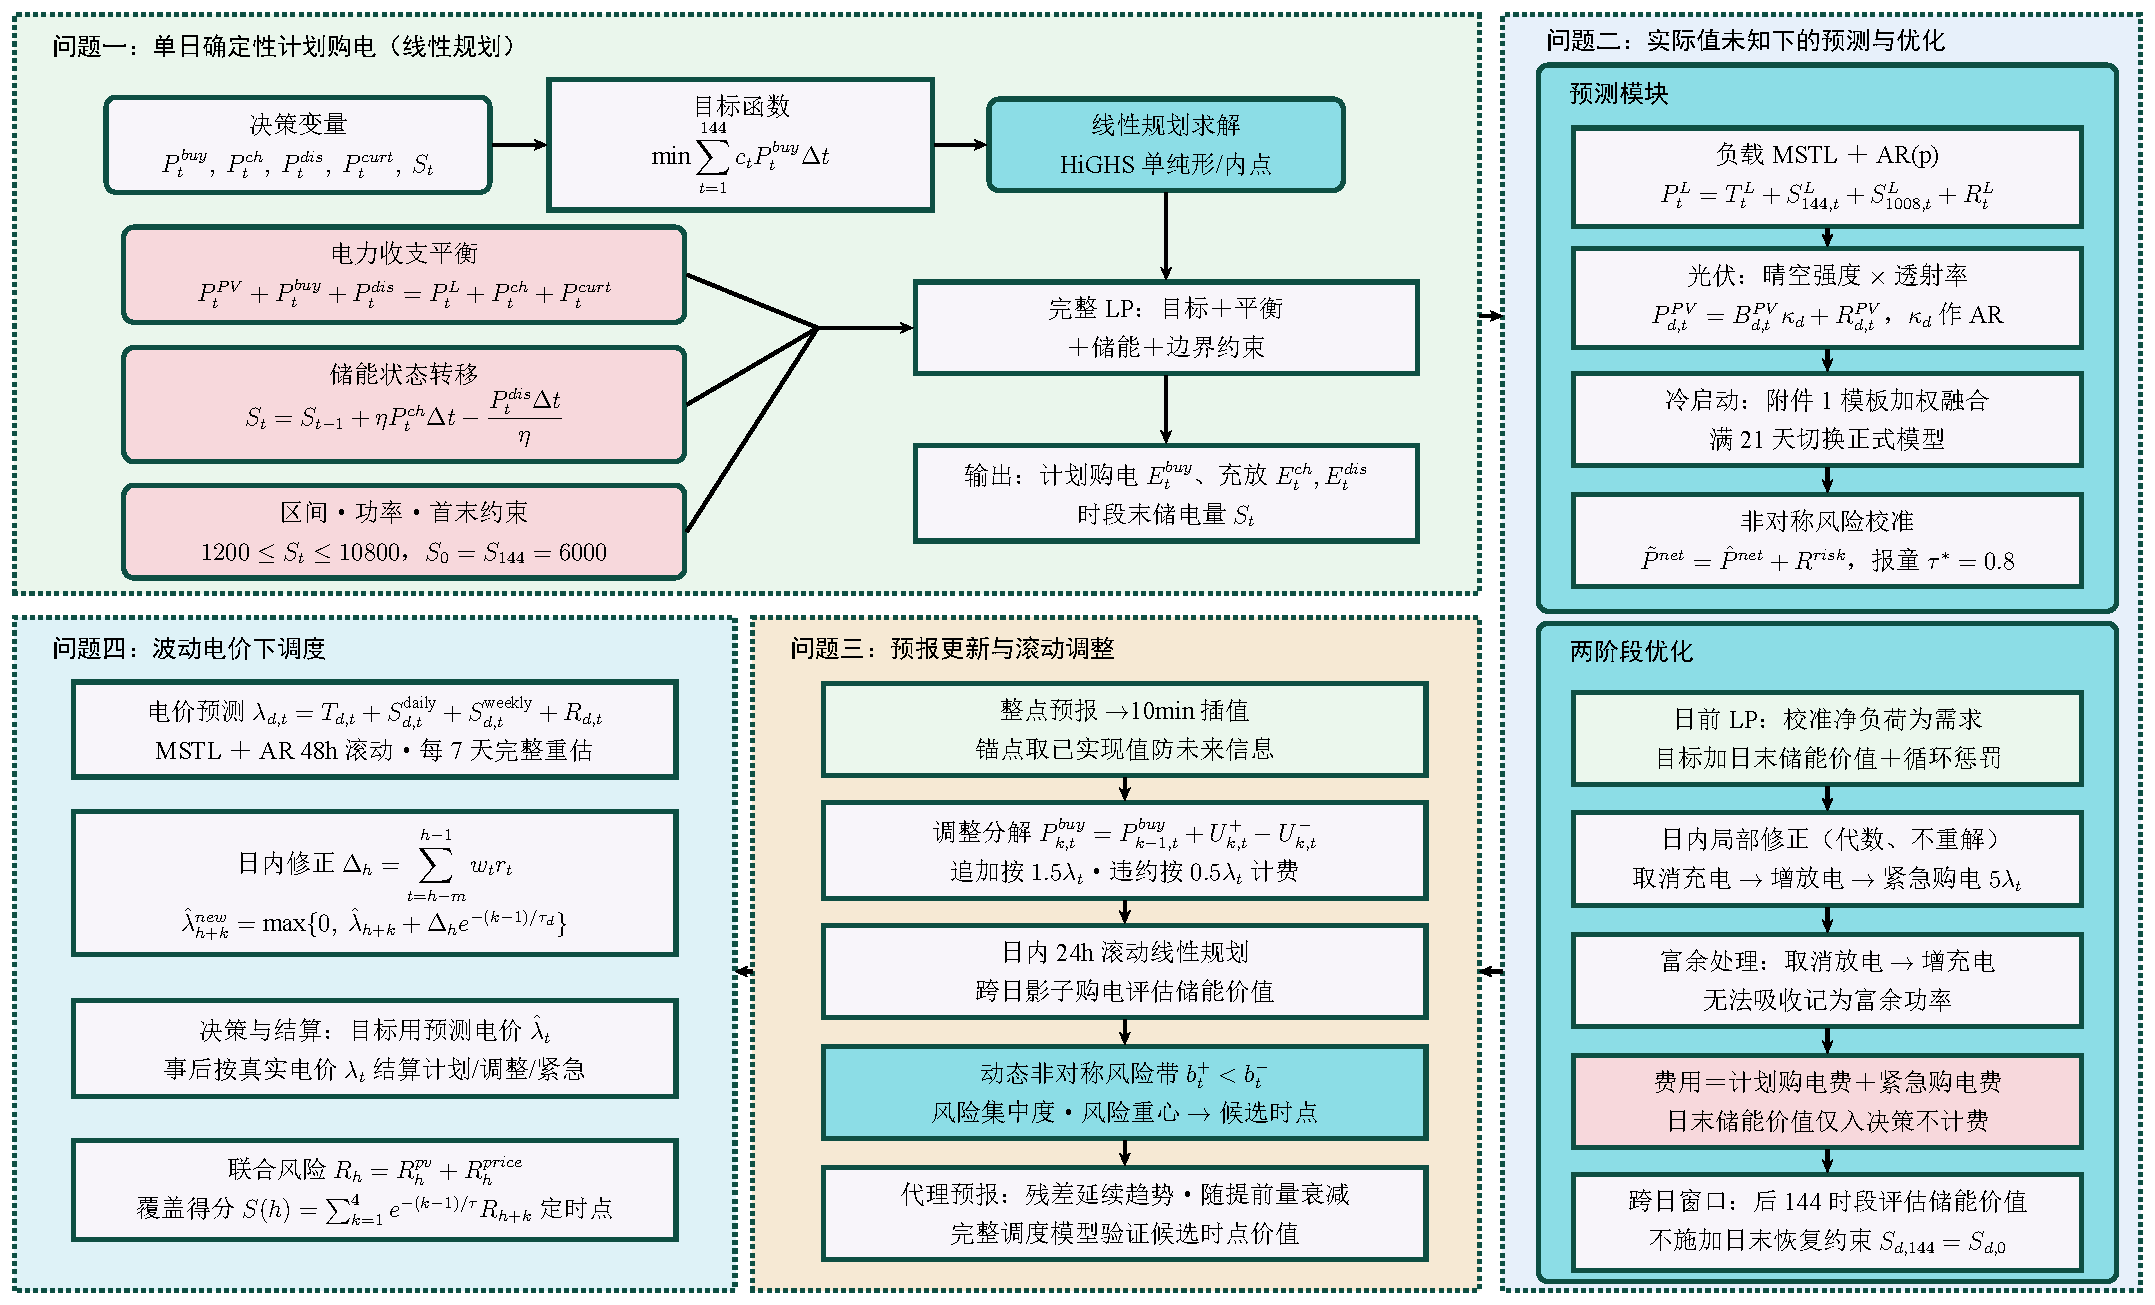
\includegraphics[
			width=1\textwidth,
			trim=0cm 0cm 0cm 0cm,
			clip
			]{figures/26国赛流程图.pdf}
			\caption{问题求解流程图}
			\label{fig:流程图}
		\end{figure}
	\end{lstlisting}
	
	\begin{figure}[h!]
		\centering
		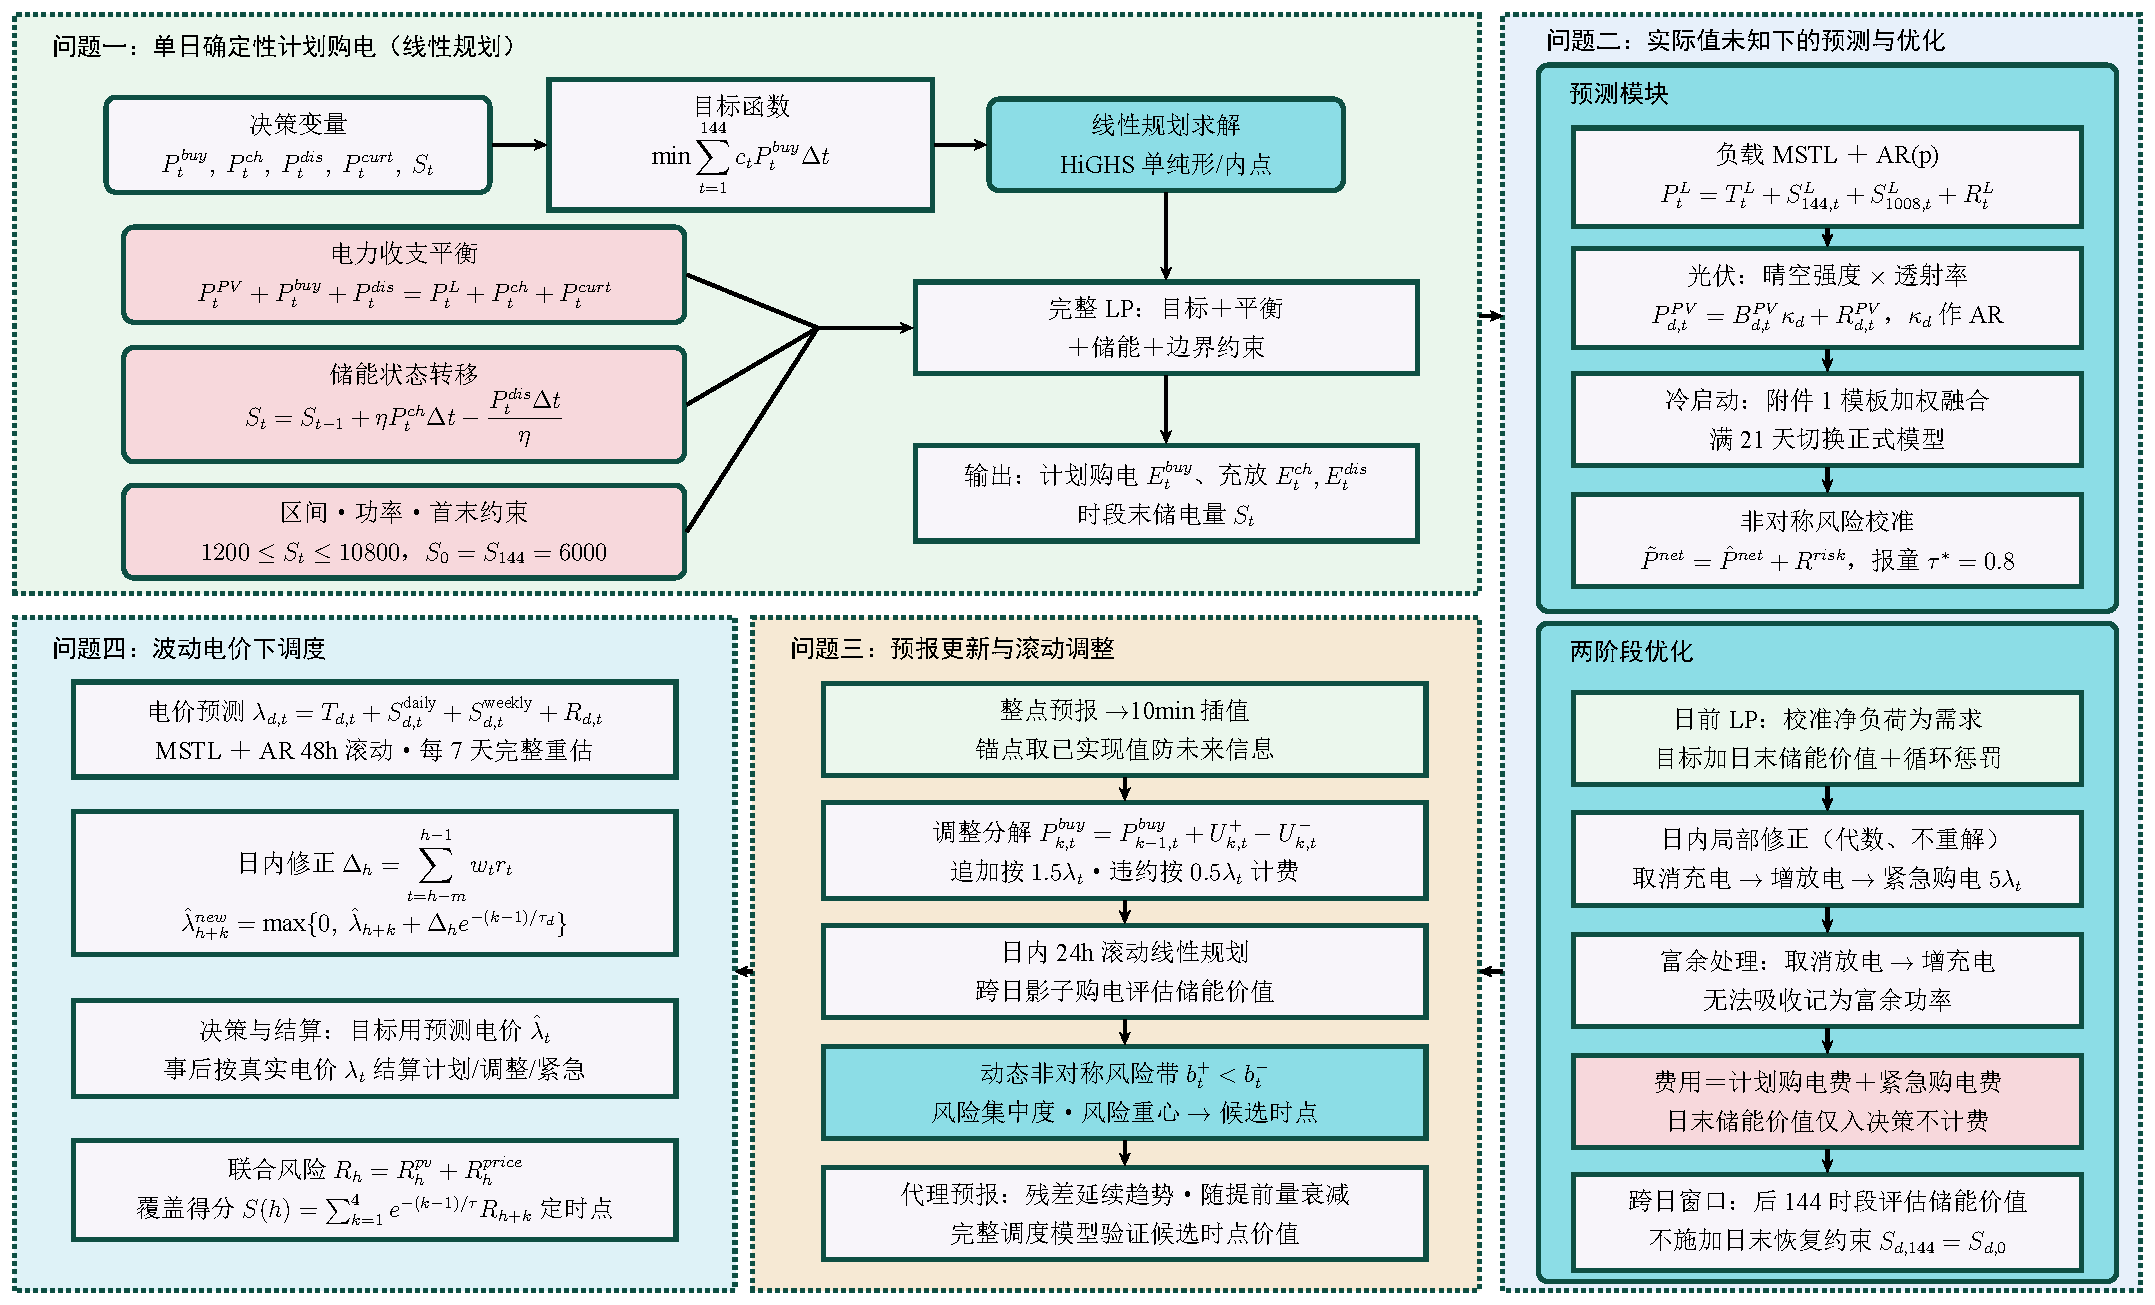
\includegraphics[
		width=1\textwidth,
		trim=0cm 0cm 0cm 0cm,
		clip
		]{figures/26国赛流程图.pdf}
		\caption{问题求解流程图}
		\label{fig:流程图}
	\end{figure}
	
	\textbf{参数说明：}
	
	\begin{itemize}
		\item \verb|trim=左 下 右 上|：从四个方向裁剪掉多余的白边，单位为 cm。例如 \verb|trim=1cm 0.5cm 1cm 0.5cm| 表示左边裁掉 $1$ cm、下边裁掉 $0.5$ cm、右边裁掉 $1$ cm、上边裁掉 $0.5$ cm。
		\item \verb|clip|：必须与 \verb|trim| 搭配使用，表示“启用裁剪”。若不加 \verb|clip|，\verb|trim| 不生效。
		\item \verb|width=1\textwidth|：图片占满整个文字区域宽度。
	\end{itemize}
	
	\subsection{单图插入（PNG 格式）}
	
	PNG 为位图格式，适合截图、数据可视化等。用法与 PDF 完全相同，只是文件后缀不同：
	
	\begin{lstlisting}
		\begin{figure}[h!]
			\centering
			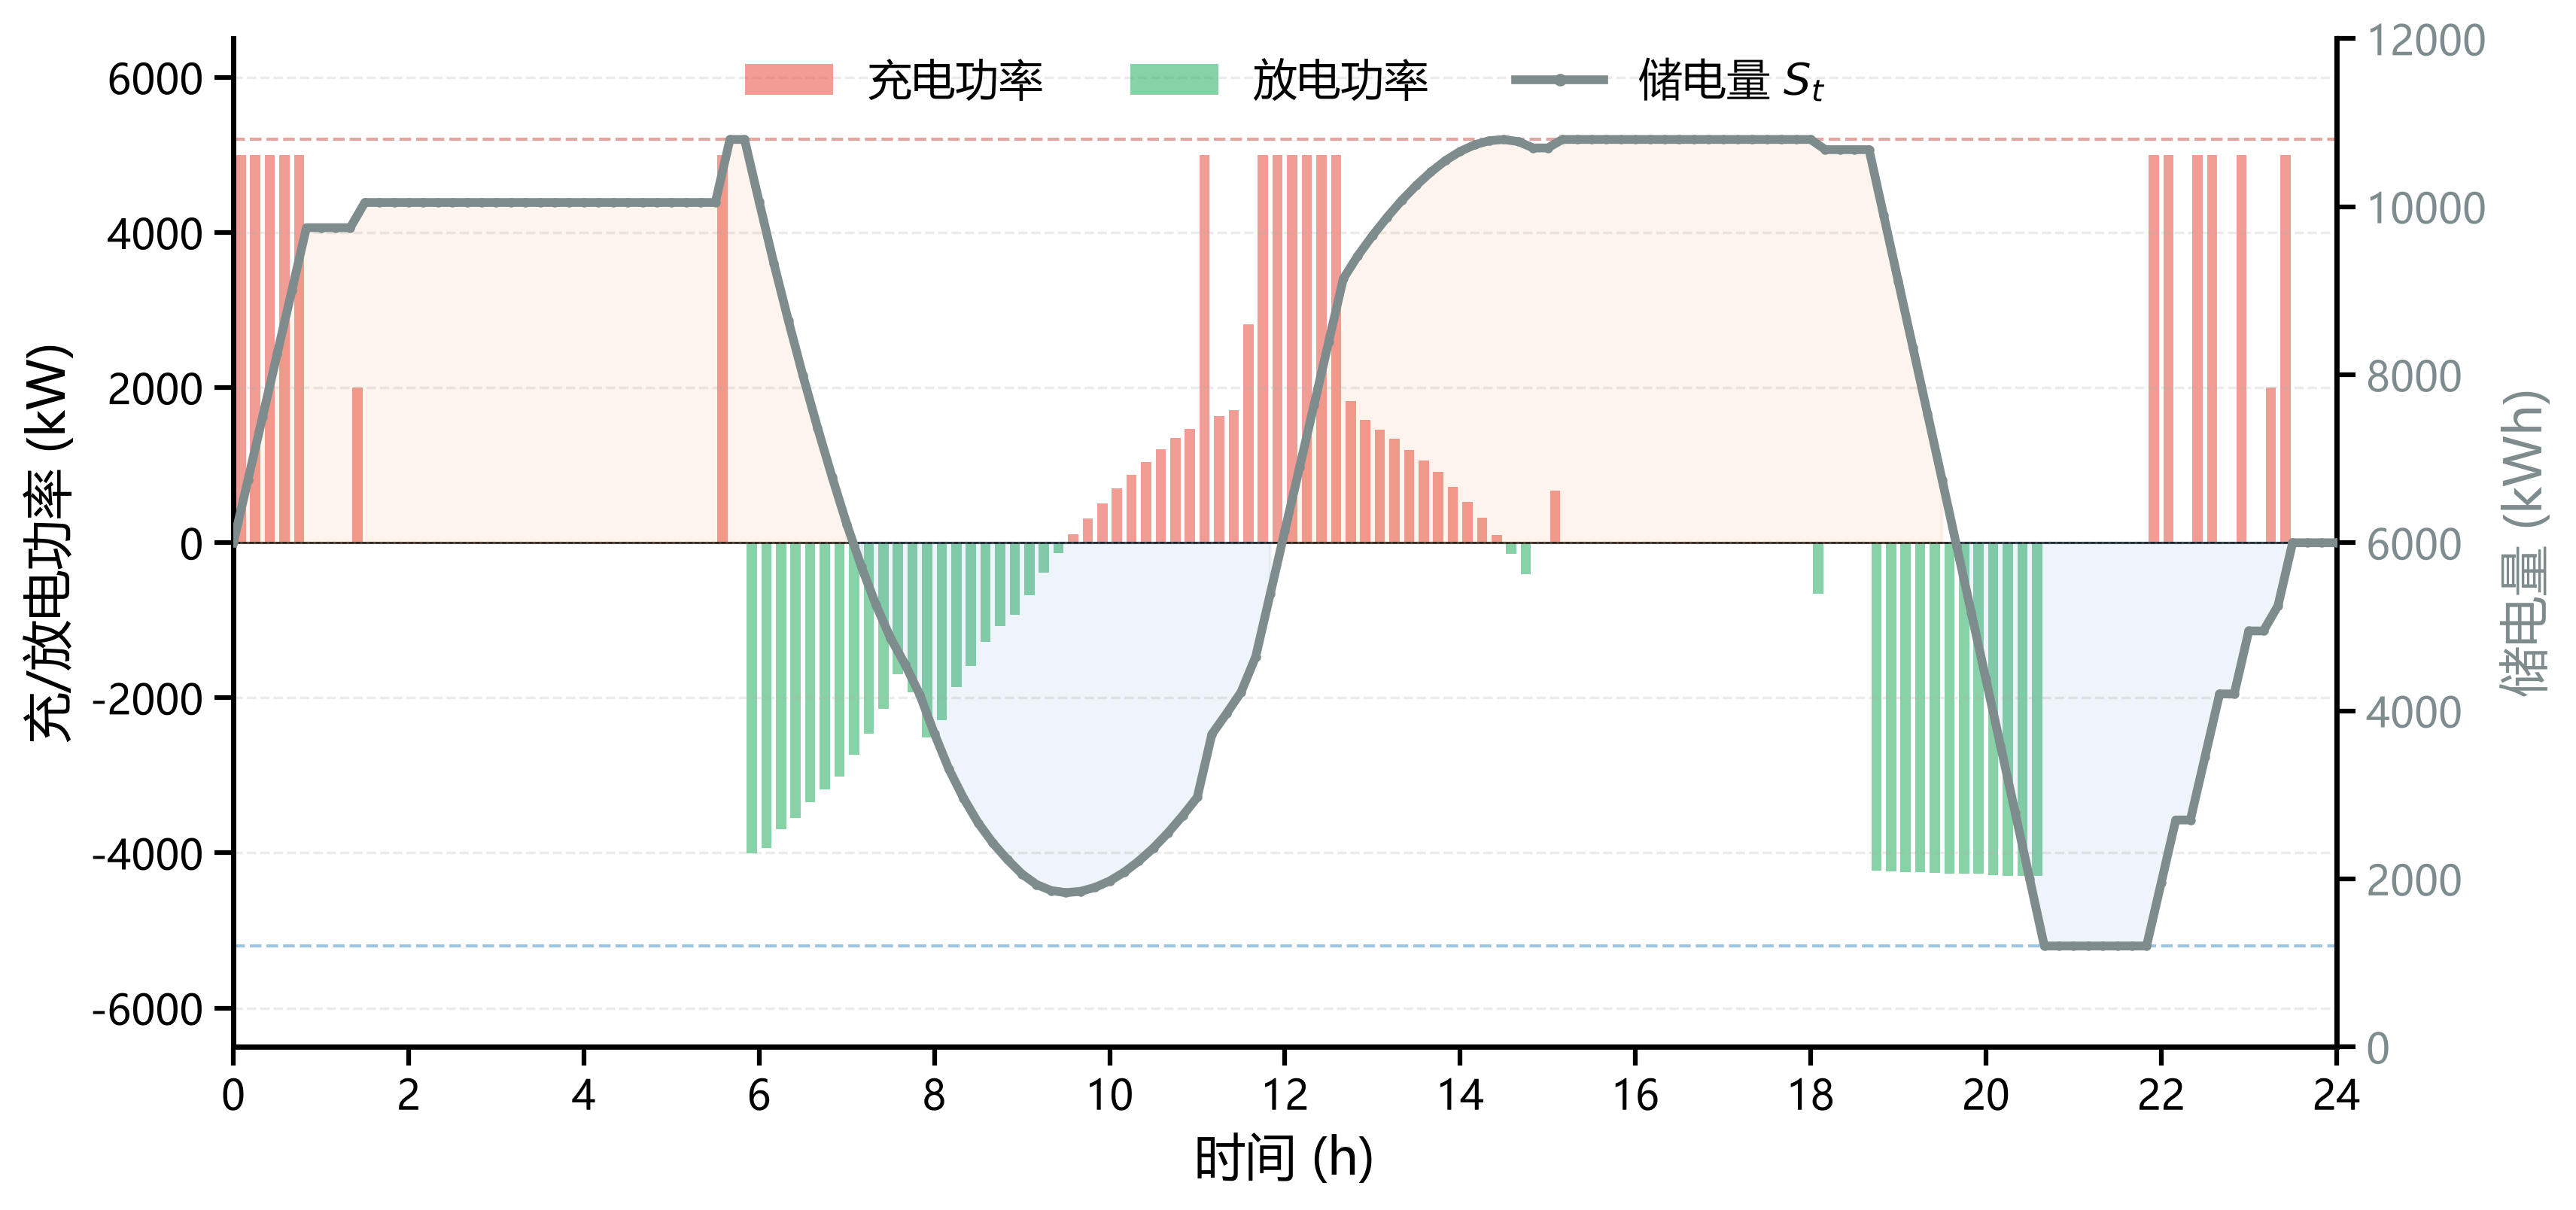
\includegraphics[width=.7\textwidth]{figures/第一问储能充放电.png}
			\caption{问题一储能设备充放电功率与储电量轨迹}
			\label{fig:充放电}
		\end{figure}
	\end{lstlisting}
	
	\begin{figure}[h!]
		\centering
		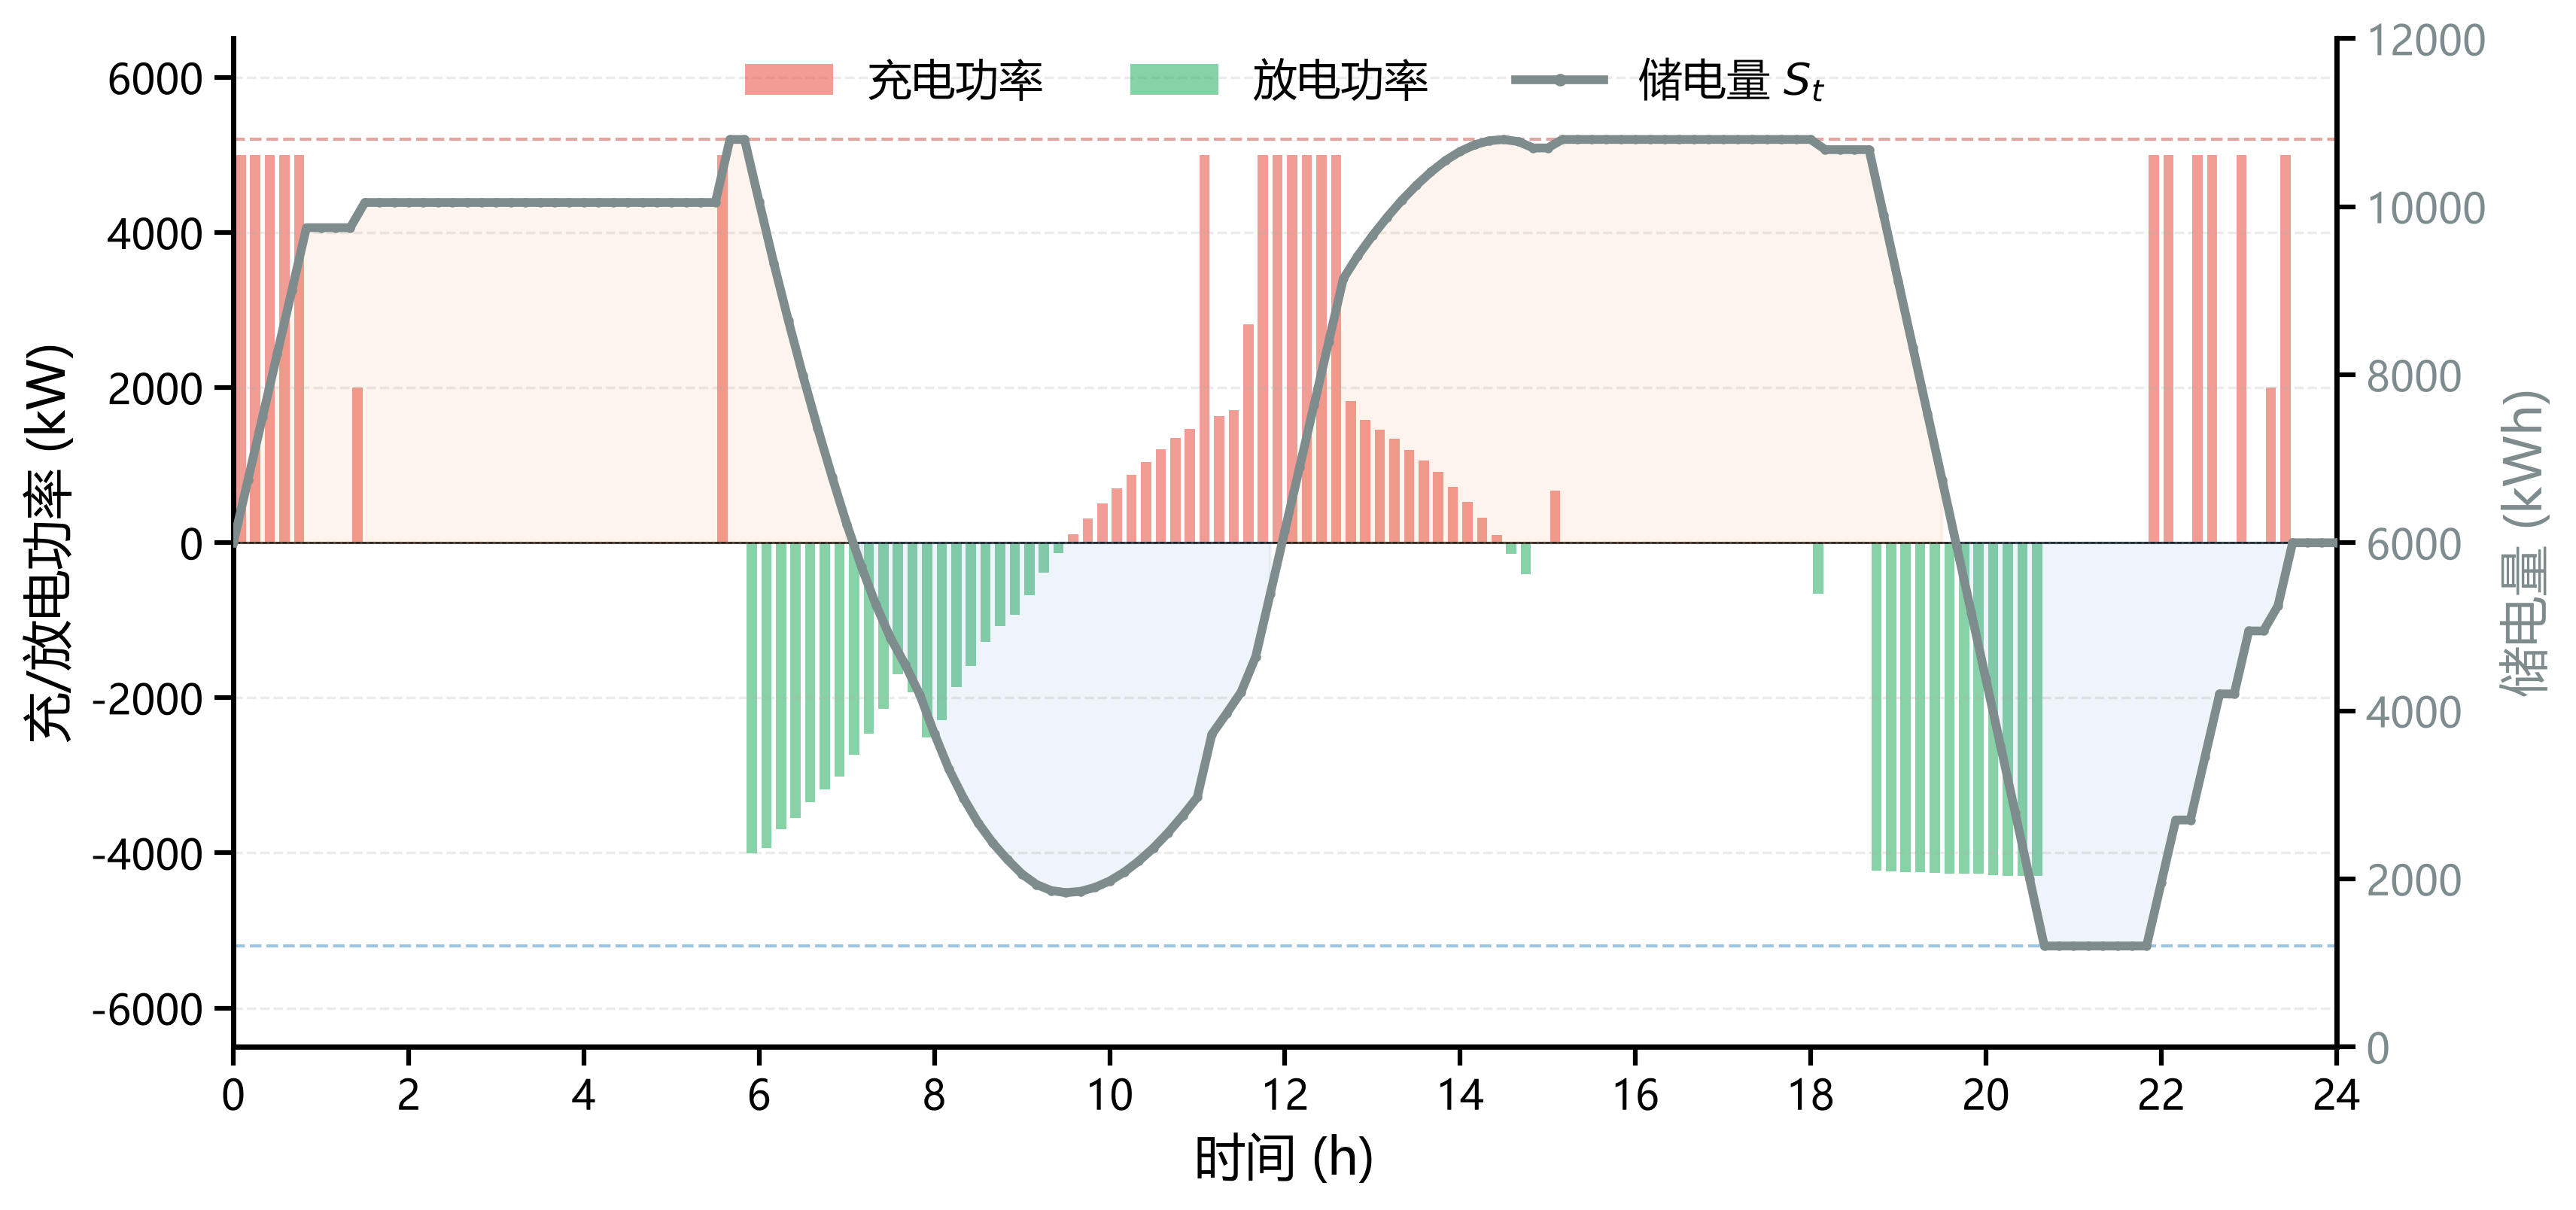
\includegraphics[width=.7\textwidth]{figures/第一问储能充放电.png}
		\caption{问题一储能设备充放电功率与储电量轨迹}
		\label{fig:充放电}
	\end{figure}
	
	\textbf{说明：}
	\begin{itemize}
		\item 图片文件名中避免使用空格和特殊字符，建议用英文或拼音命名。
		\item 支持格式：\verb|.pdf|、\verb|.png|、\verb|.jpg|、\verb|.eps|。
	\end{itemize}
	
	\subsection{双图并排（minipage 方式）}
	
	两张图片左右并排，各自拥有独立的标题和编号：
	
	\begin{lstlisting}
		\begin{figure}[h!]
			\centering
			\begin{minipage}{0.6\textwidth}
				\centering
				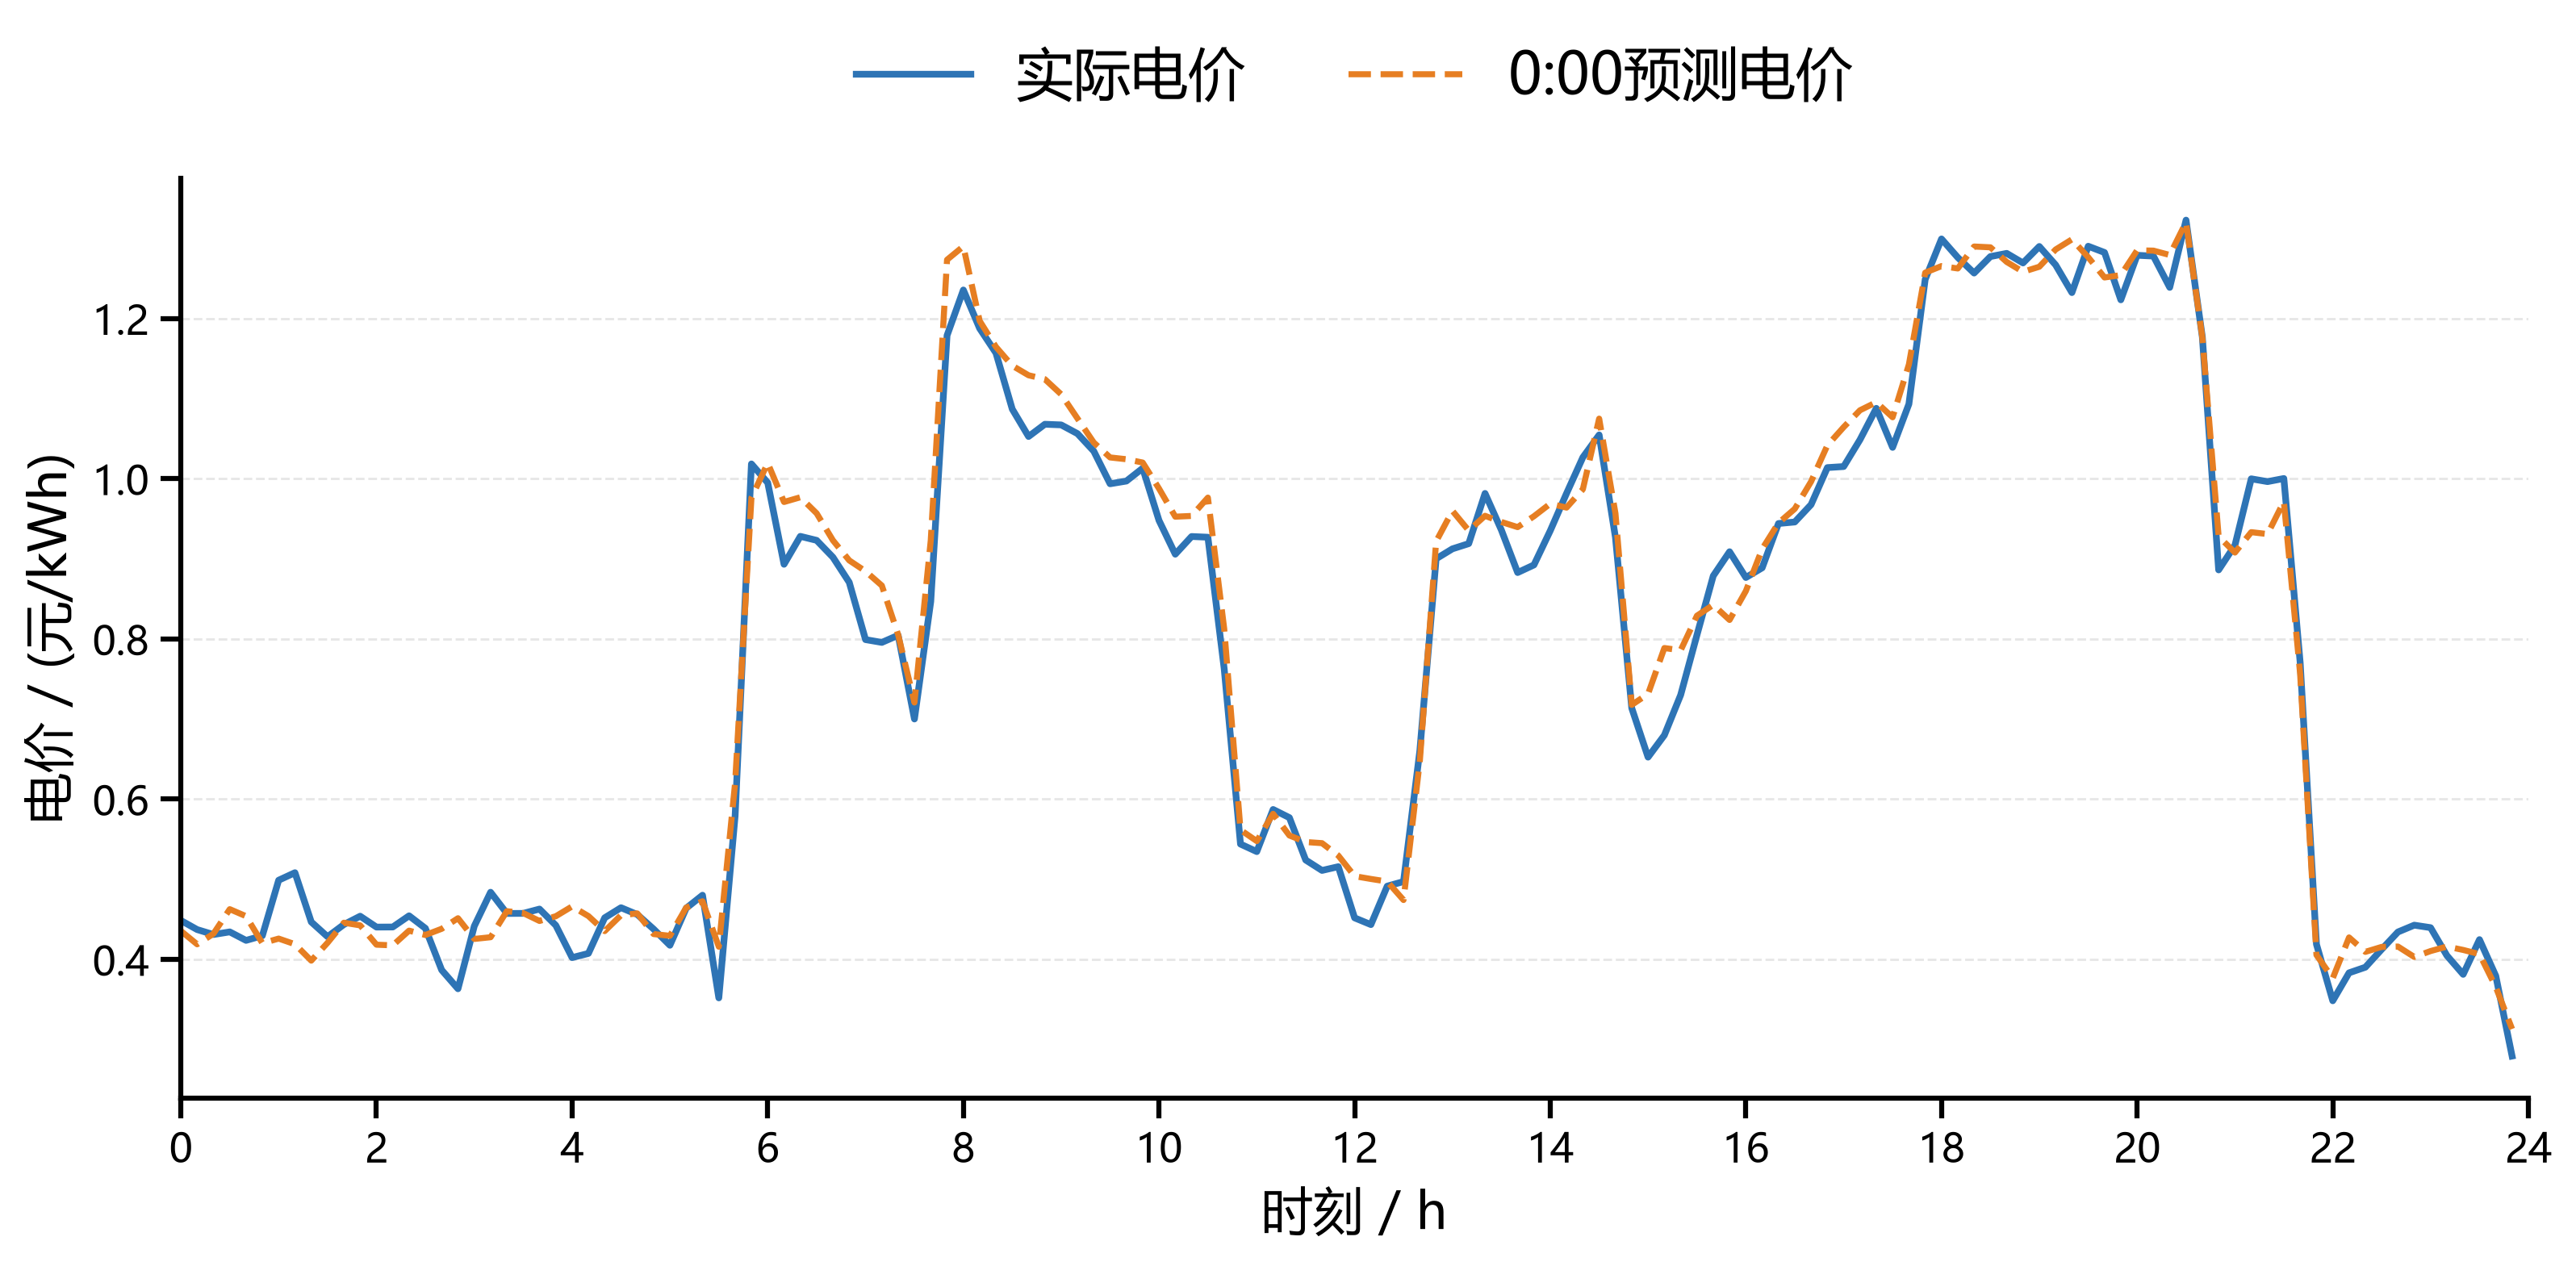
\includegraphics[width=\linewidth]{figures/第四问3-20波动电价预测对比.png}
				\caption{3月20日波动电价预测对比}
				\label{fig:电价对比}
			\end{minipage}
			\hfill
			\begin{minipage}{0.3\textwidth}
				\centering
				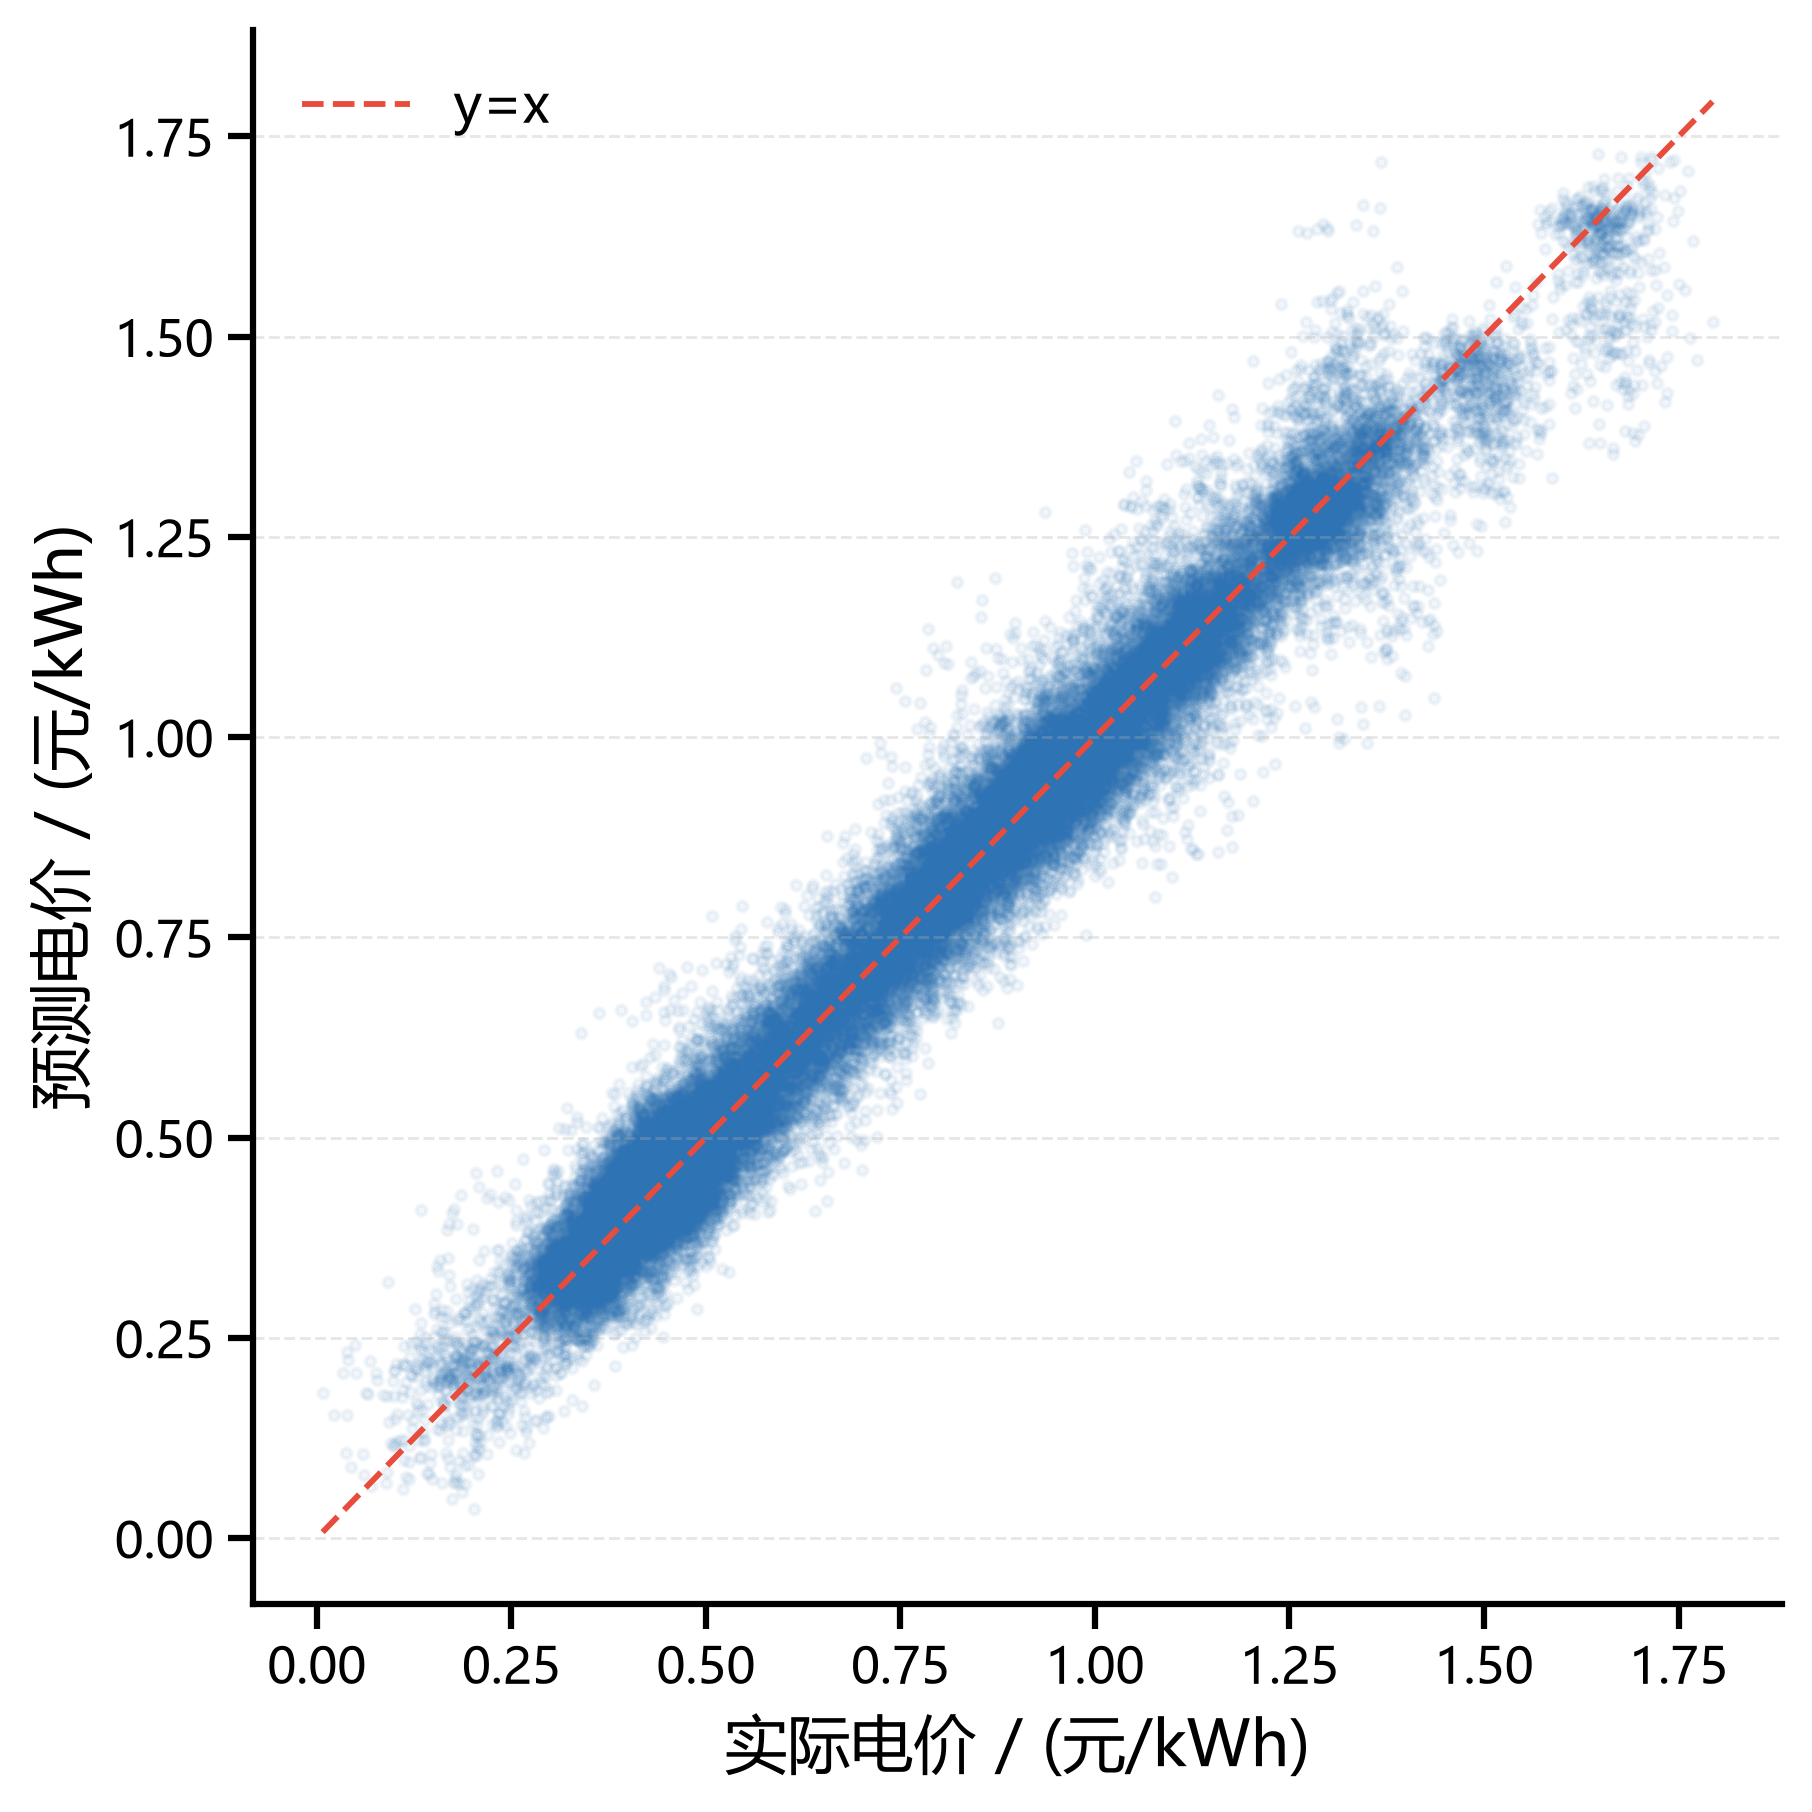
\includegraphics[width=\linewidth]{figures/第四问全年10分钟级电价预测一致性.png}
				\caption{电价预测一致性}
				\label{fig:电价一致性}
			\end{minipage}
		\end{figure}
	\end{lstlisting}
	
	\begin{figure}[h!]
		\centering
		\begin{minipage}{0.6\textwidth}
			
			\centering
			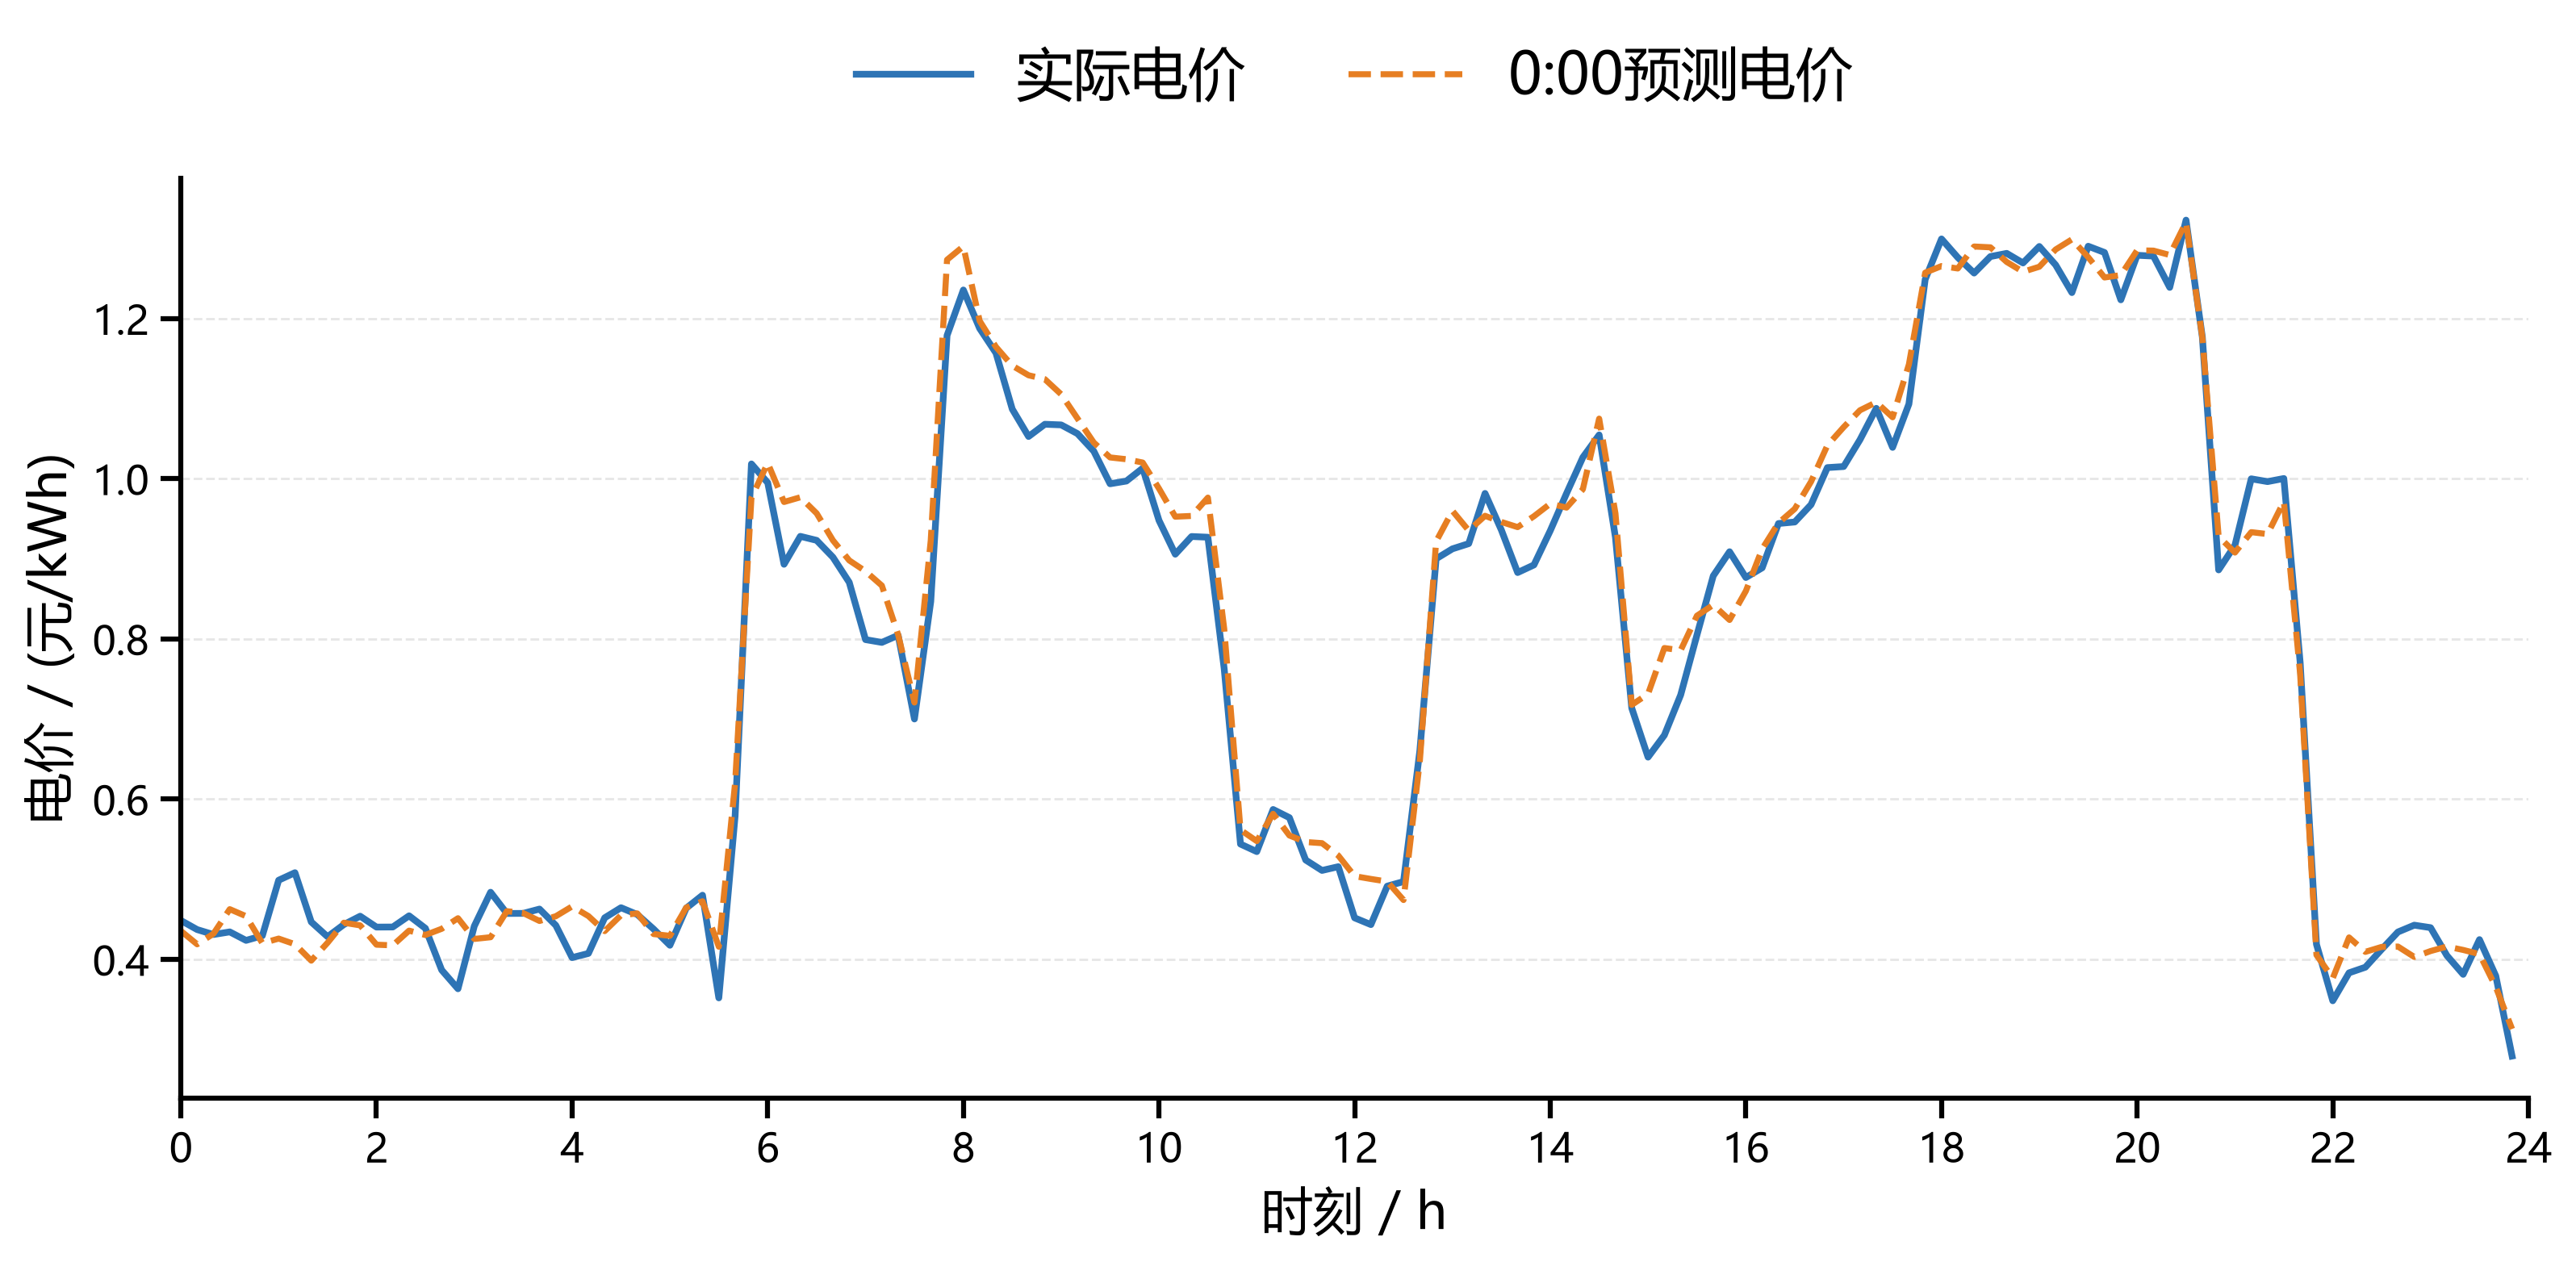
\includegraphics[width=\linewidth]{figures/第四问3-20波动电价预测对比.png}
			\caption{3月20日波动电价预测对比}
			\label{fig:电价对比}
			
		\end{minipage}
		\hfill
		\begin{minipage}{0.3\textwidth}
			
			\centering
			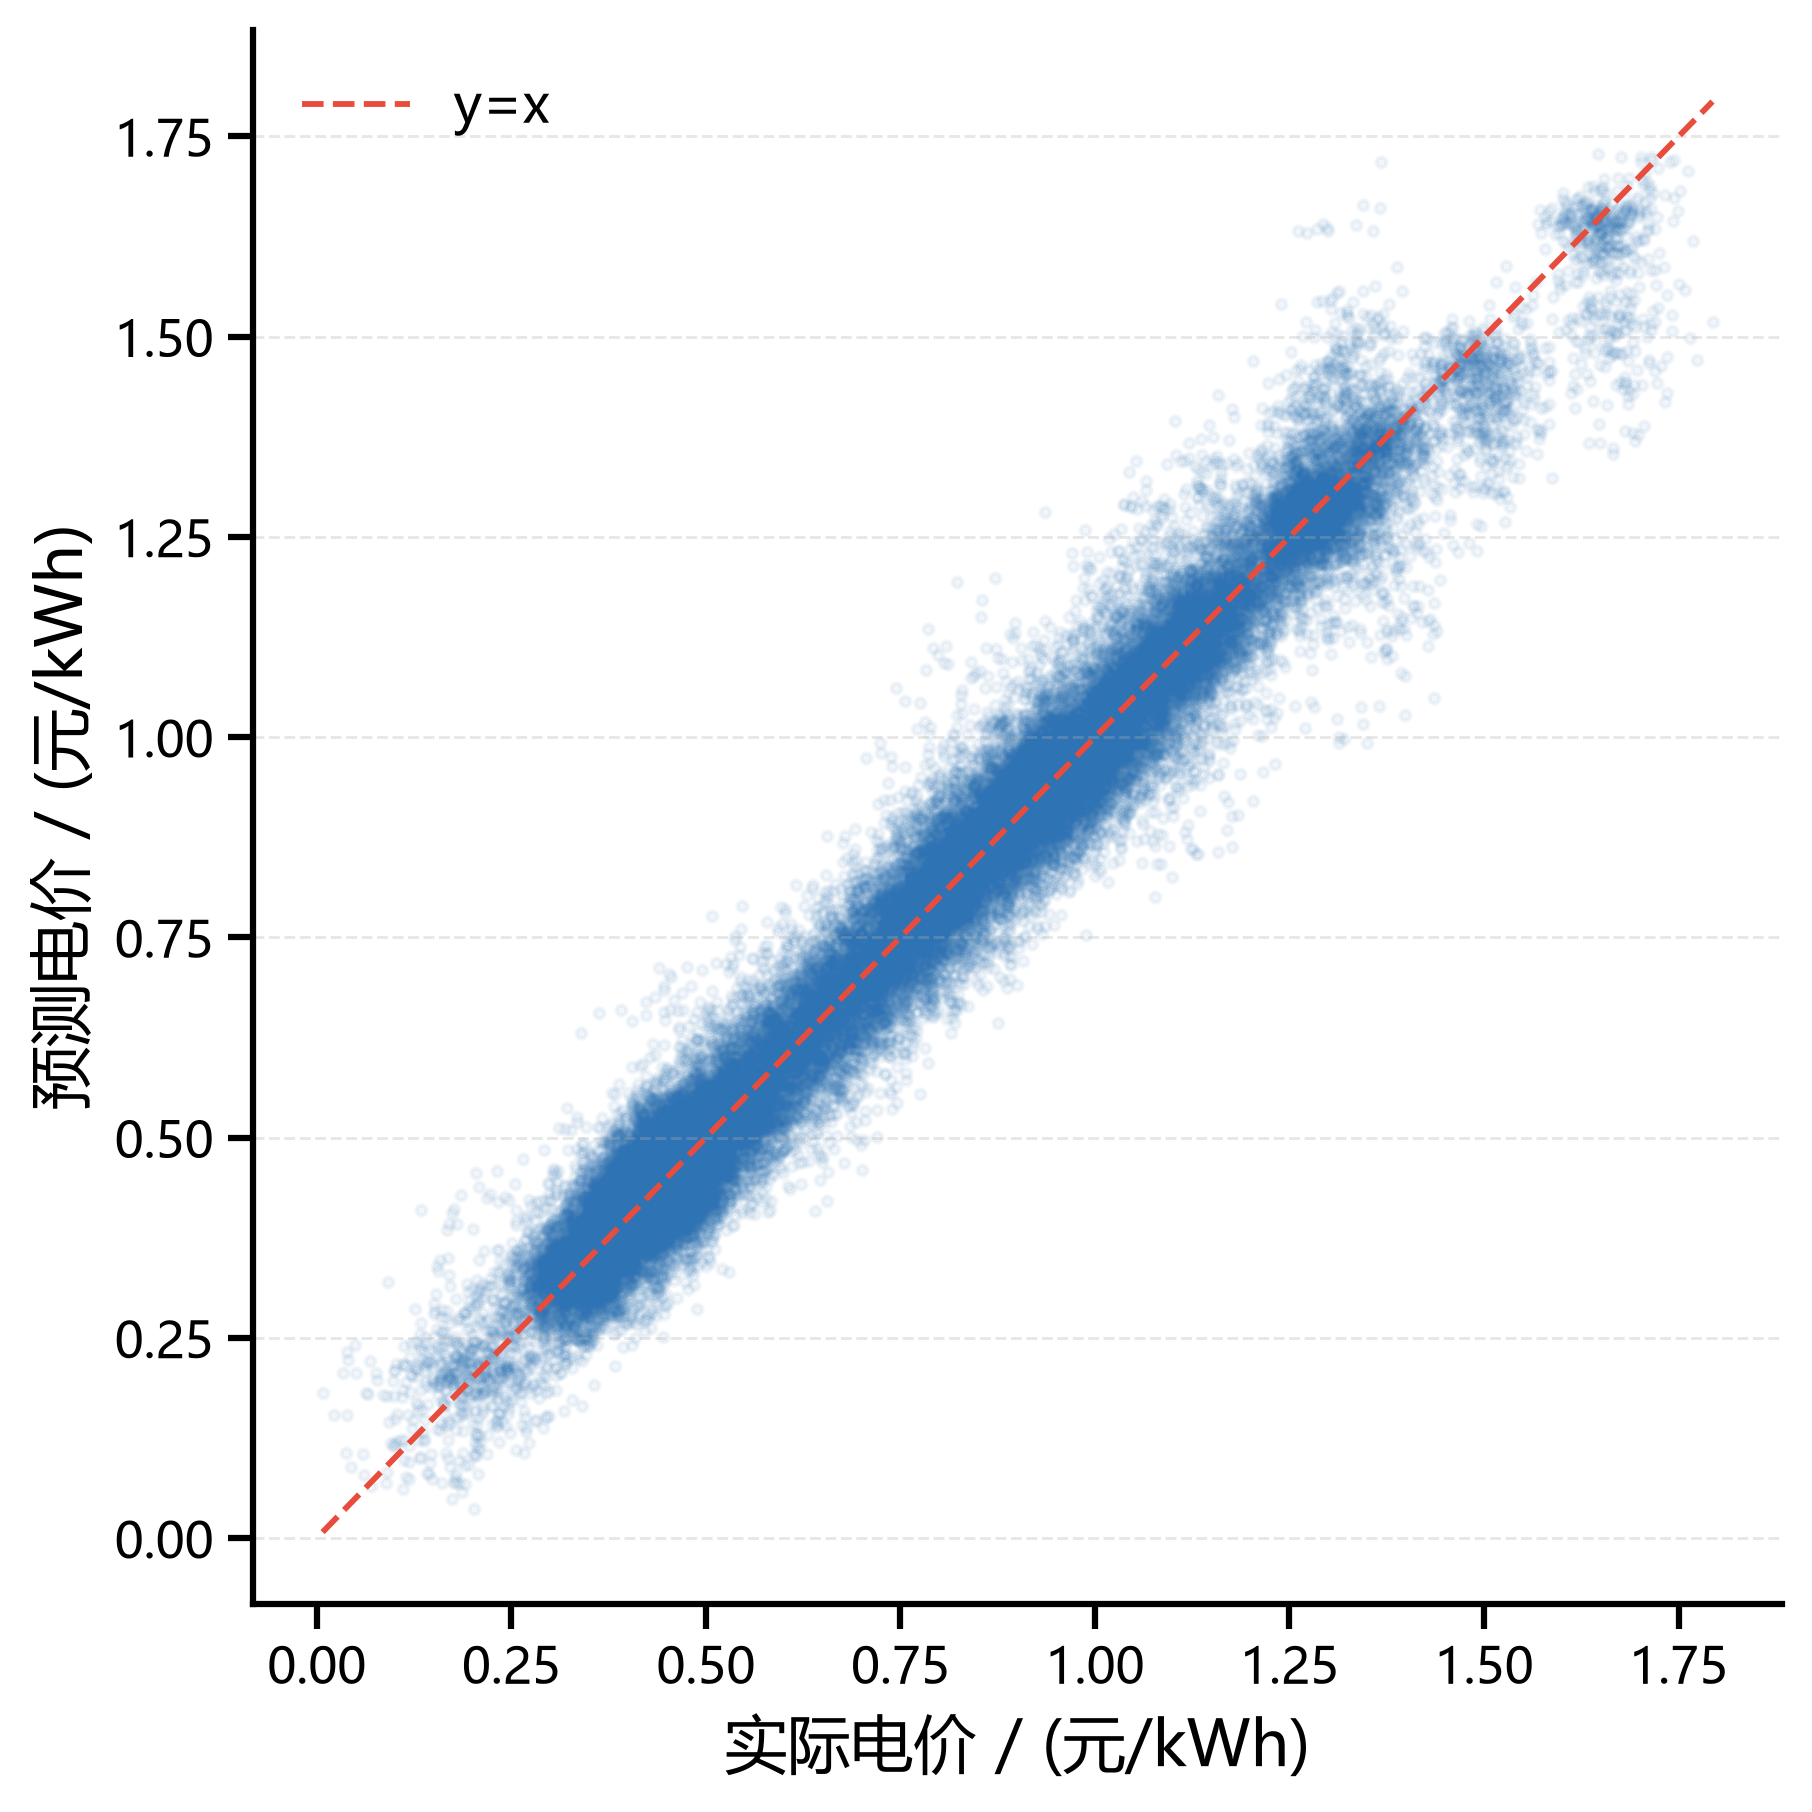
\includegraphics[width=\linewidth]{figures/第四问全年10分钟级电价预测一致性.png}
			\caption{电价预测一致性}
			\label{fig:电价一致性}
			
		\end{minipage}
	\end{figure}
	
	\textbf{要点：}
	
	\begin{itemize}
		\item 两个 \verb|minipage| 的宽度之和应略小于 \verb|1\textwidth|（如 $0.6 + 0.3 = 0.9$），留出间距。
		\item \verb|\hfill|：弹性空白，将两个 \verb|minipage| 推向两端。
		\item 每个 \verb|minipage| 内部各自写 \verb|\caption| 和 \verb|\label|，因此两张图会分别编号为“图 1”和“图 2”。
		\item 图片宽度用 \verb|\linewidth|（当前 \verb|minipage| 的宽度），而非 \verb|\textwidth|。
	\end{itemize}
	
	\subsection{子图方式（subcaption）}
	
	若希望两张图共用一个大标题，同时各自有子编号（如图 3(a)、图 3(b)），使用 \verb|subcaption| 宏包（导言区已加载）：
	
	\begin{lstlisting}
		\begin{figure}[h!]
			\centering
			\begin{subfigure}{0.6\textwidth}
				\centering
				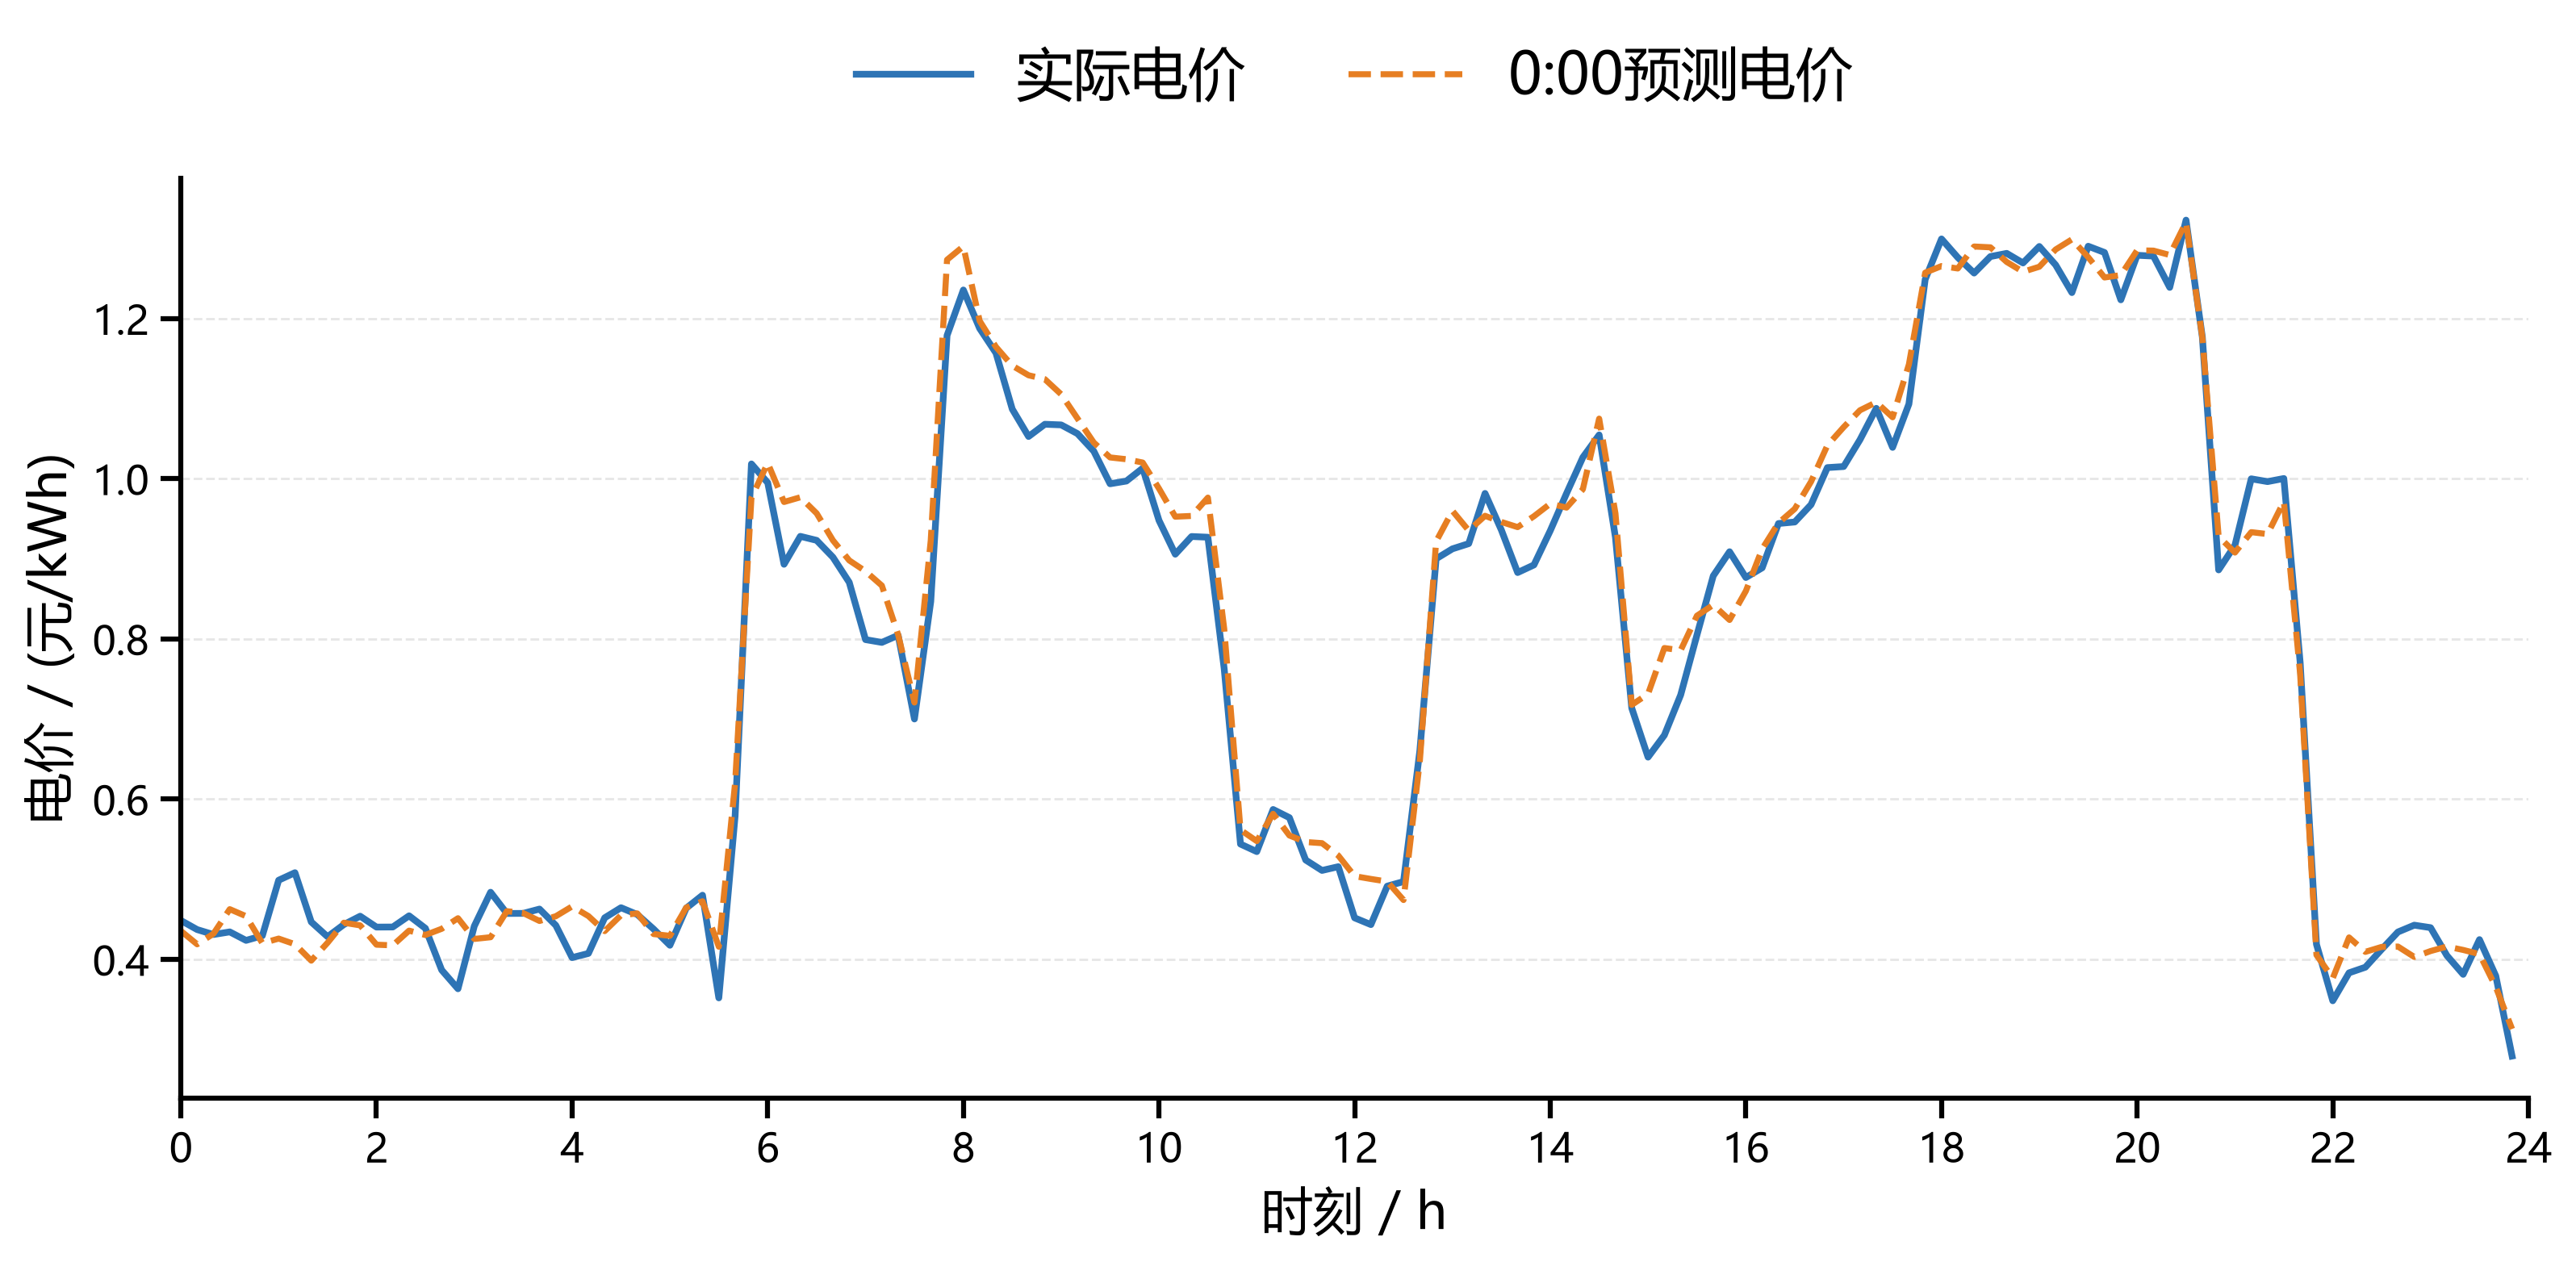
\includegraphics[width=\linewidth]{figures/第四问3-20波动电价预测对比.png}
				\caption{3月20日对比}
				\label{fig:sub_left}
			\end{subfigure}
			\hfill
			\begin{subfigure}{0.3\textwidth}
				\centering
				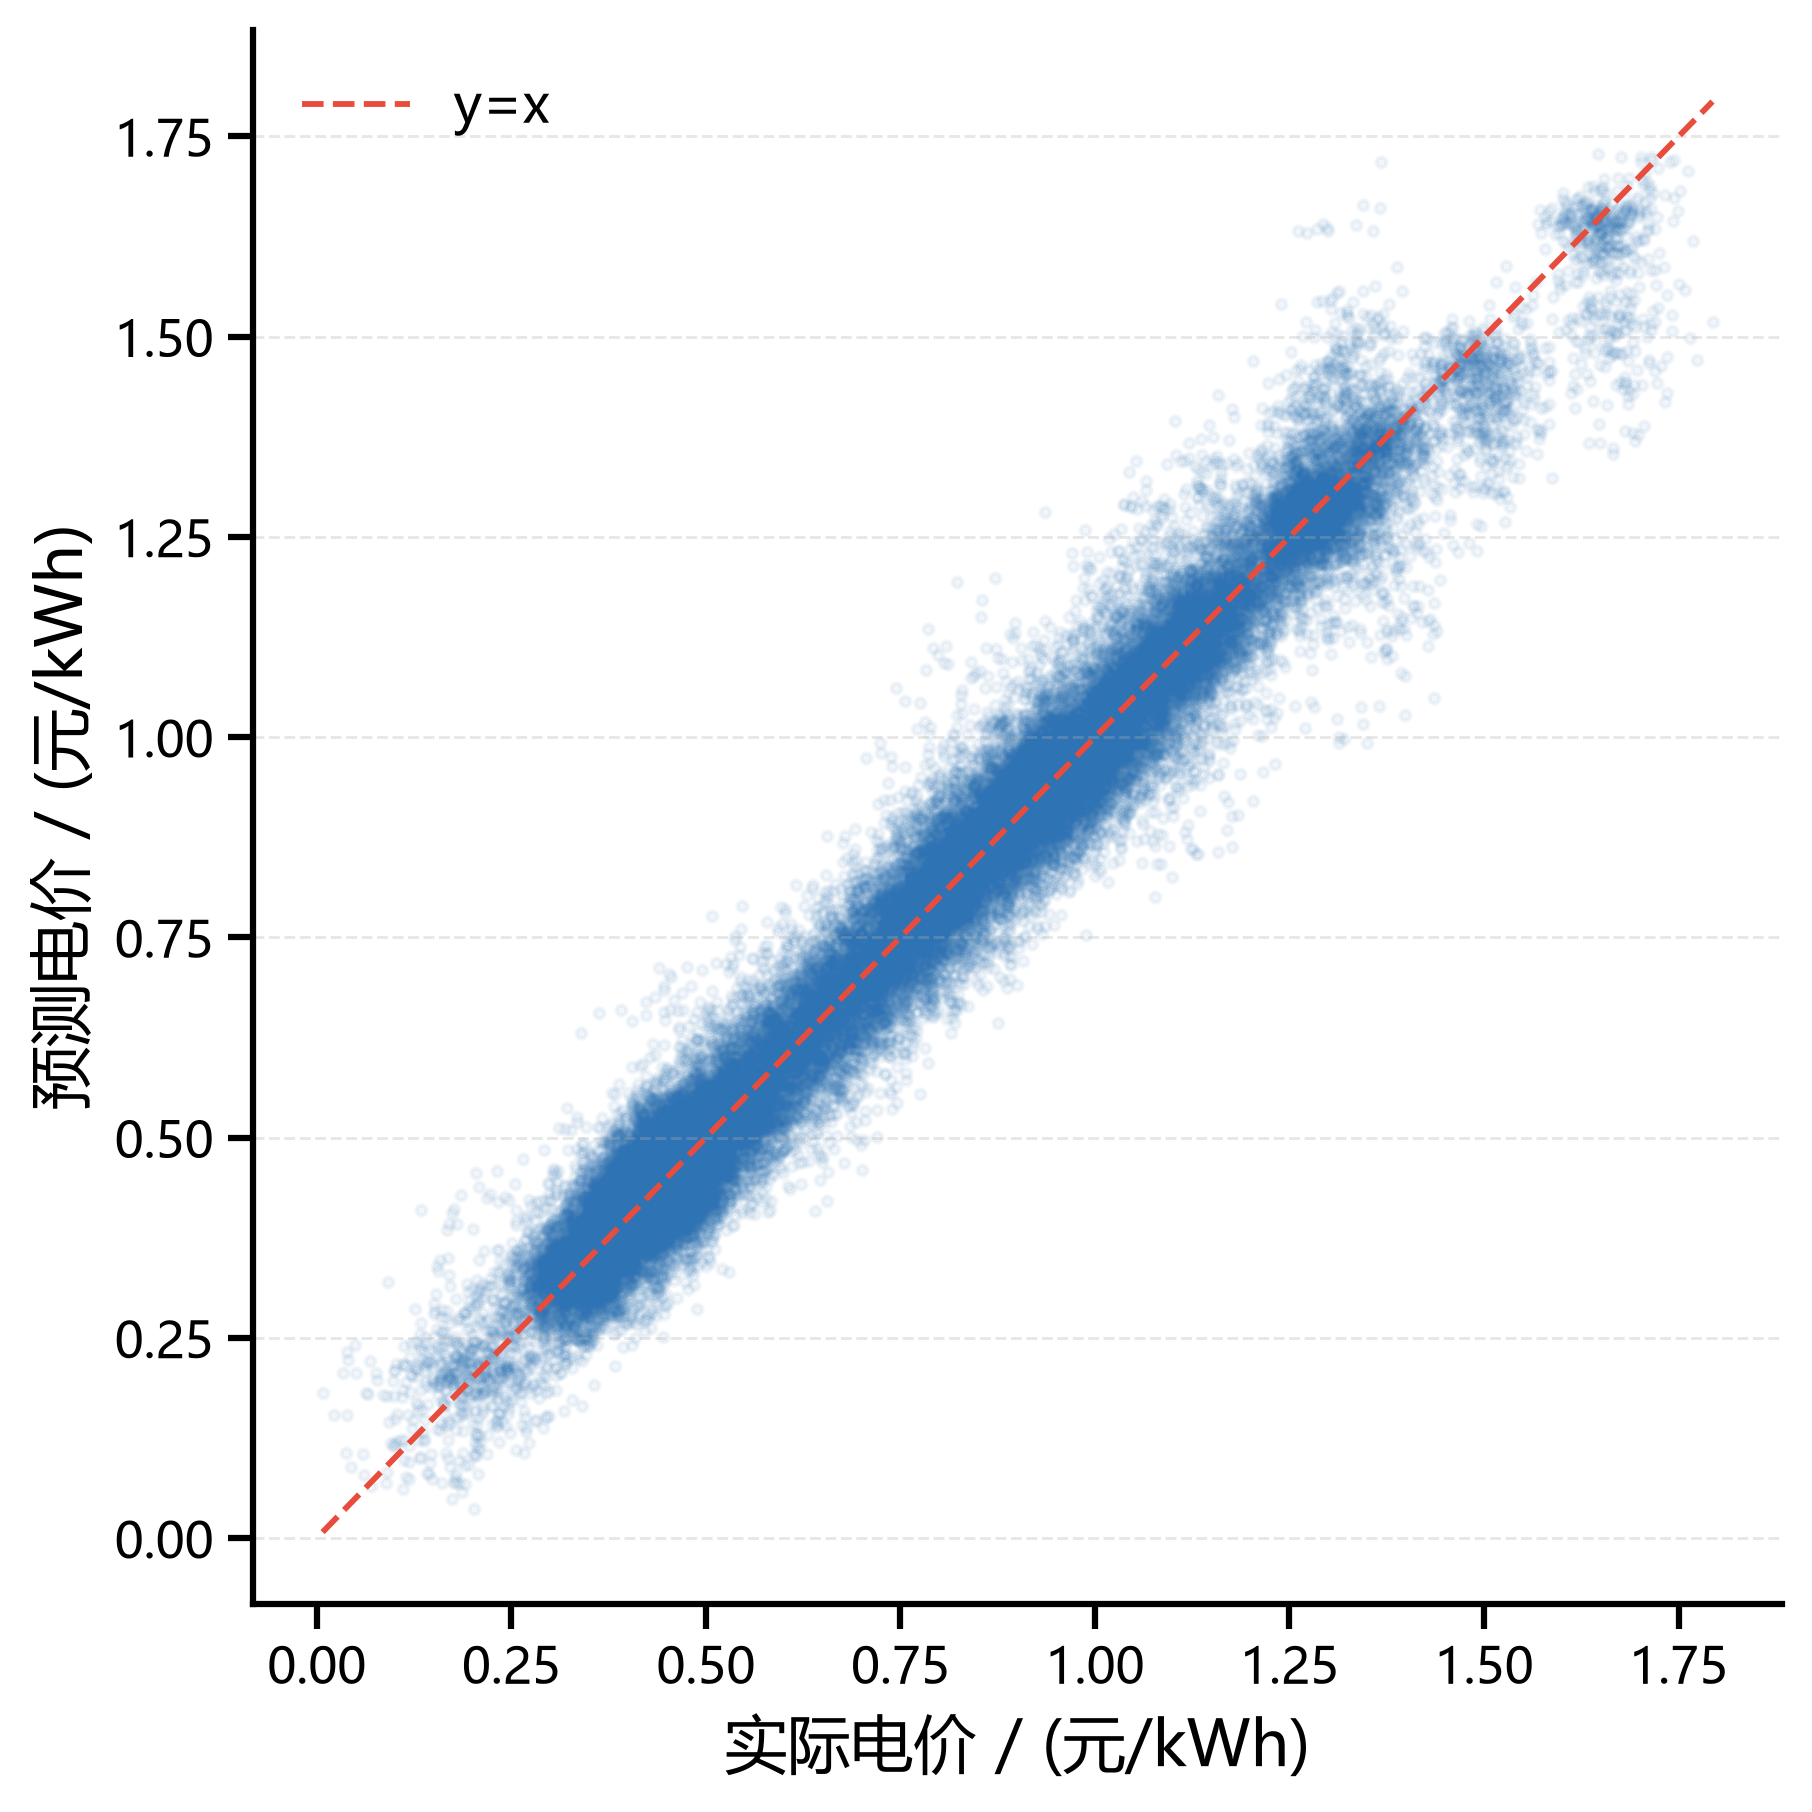
\includegraphics[width=\linewidth]{figures/第四问全年10分钟级电价预测一致性.png}
				\caption{全年一致性}
				\label{fig:sub_right}
			\end{subfigure}
			\caption{电价预测结果}
			\label{fig:电价总}
		\end{figure}
	\end{lstlisting}
	
	\begin{figure}[h!]
		\centering
		\begin{subfigure}{0.6\textwidth}
			
			\centering
			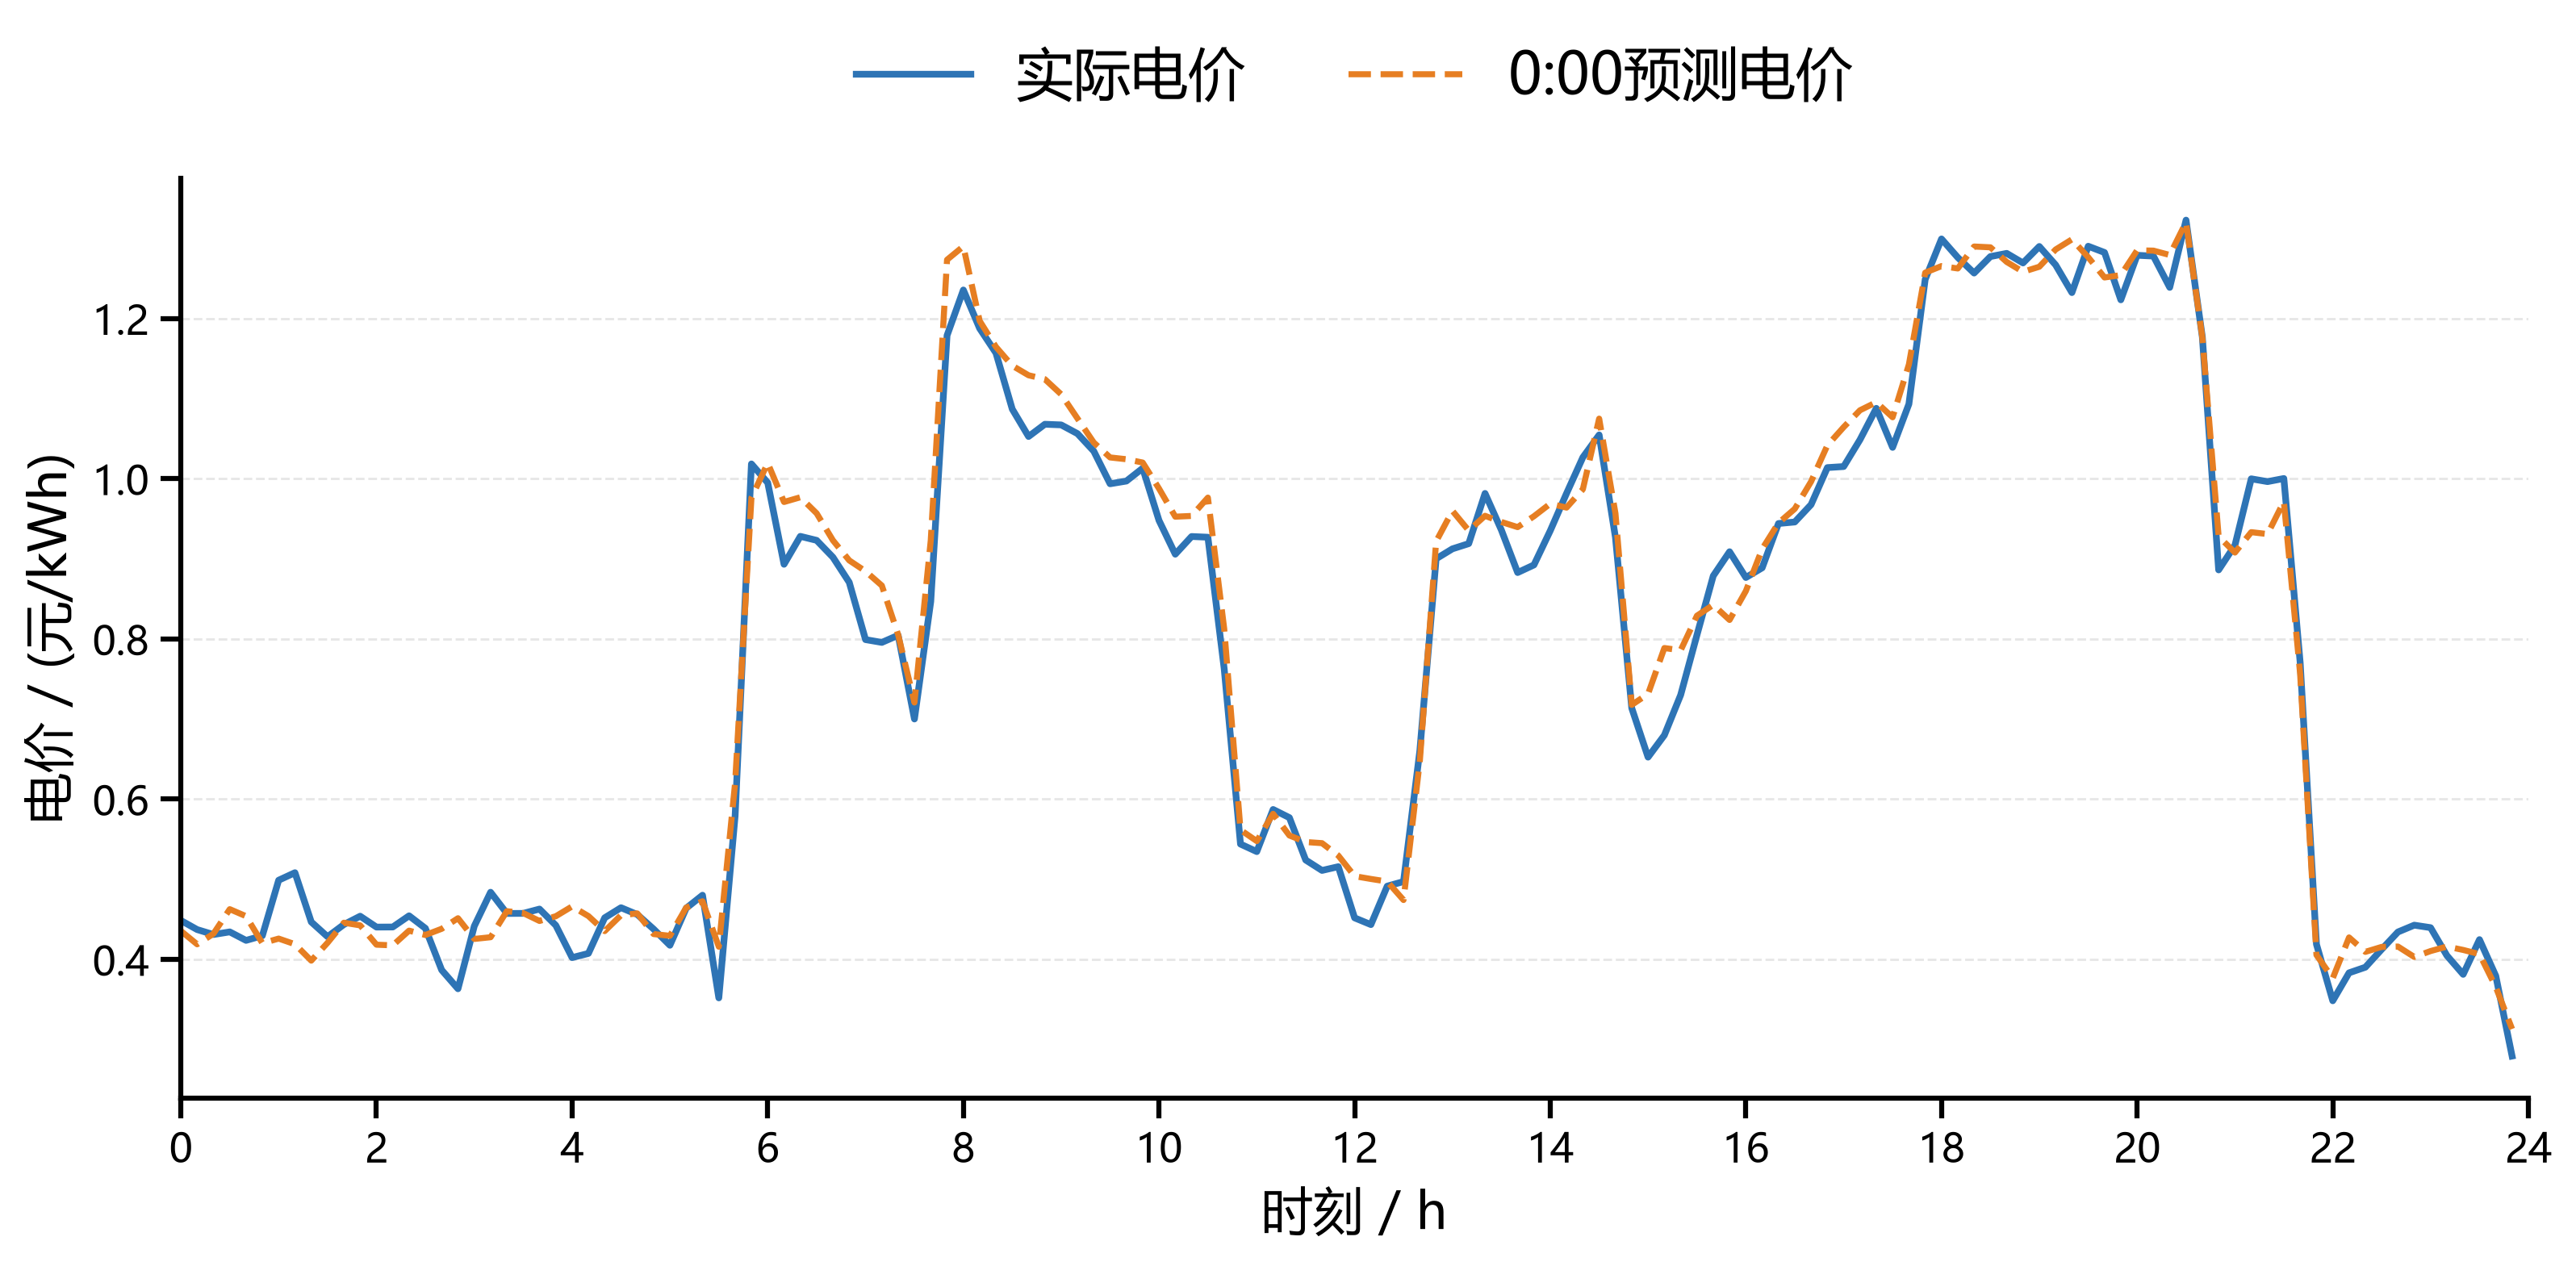
\includegraphics[width=\linewidth]{figures/第四问3-20波动电价预测对比.png}
			\caption{3月20日对比}
			\label{fig:sub_left}
			
		\end{subfigure}
		\hfill
		\begin{subfigure}{0.3\textwidth}
			
			\centering
			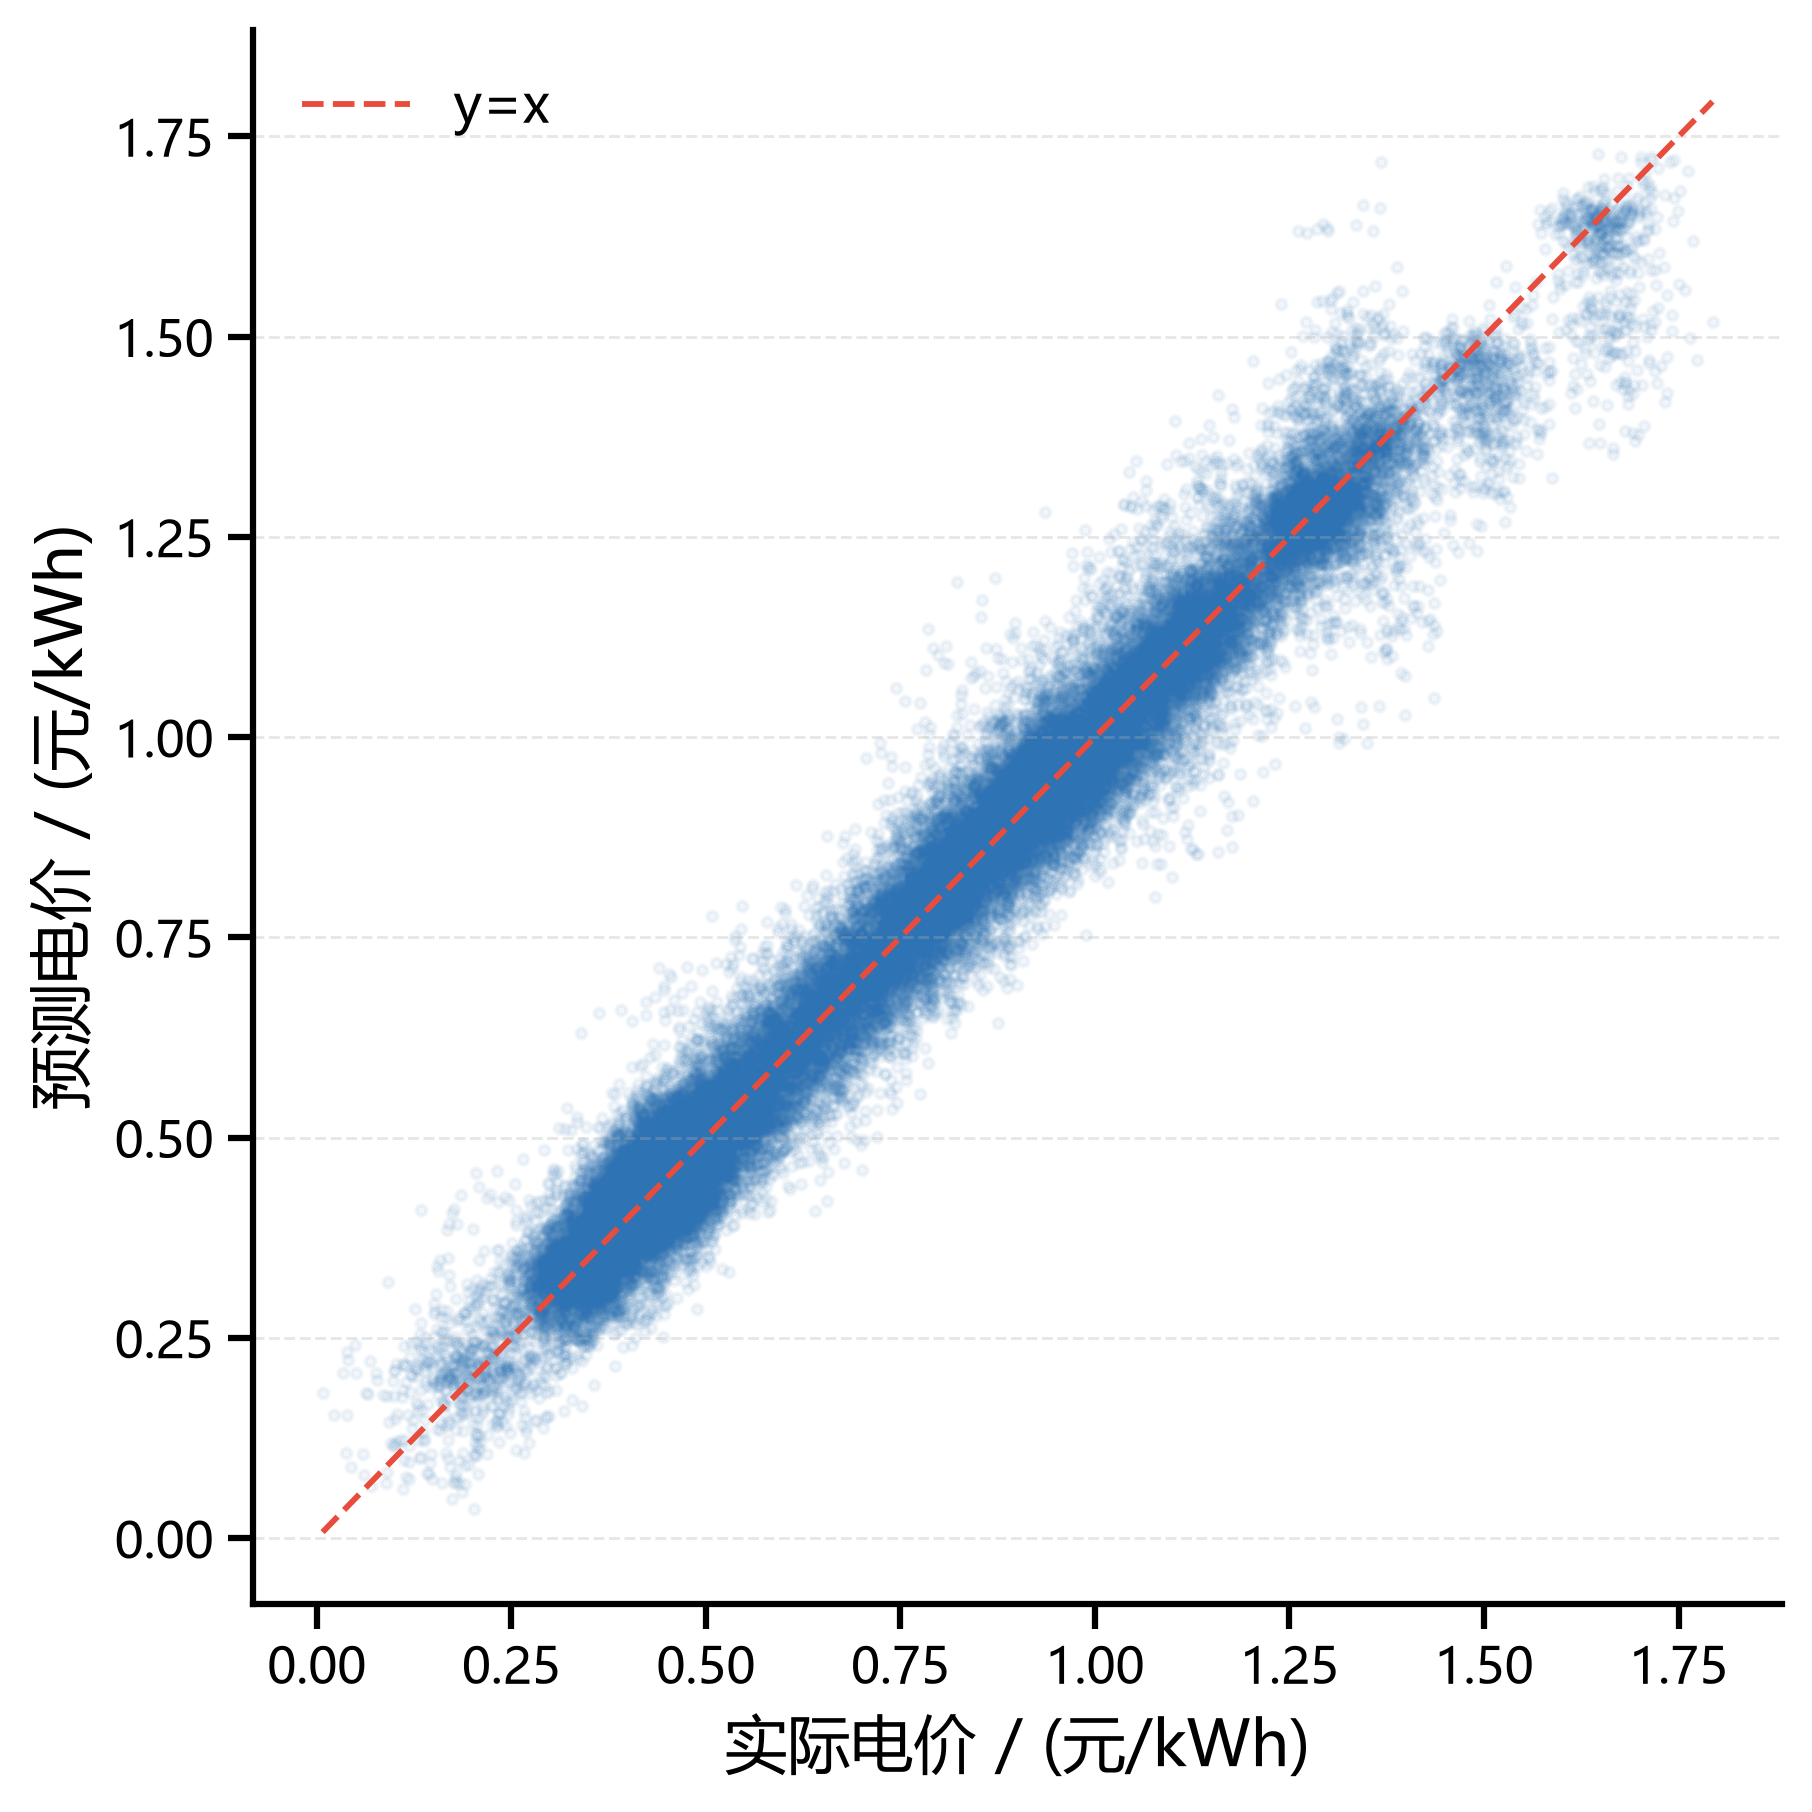
\includegraphics[width=\linewidth]{figures/第四问全年10分钟级电价预测一致性.png}
			\caption{全年一致性}
			\label{fig:sub_right}
			
		\end{subfigure}
		\caption{电价预测结果}
		\label{fig:电价总}
	\end{figure}
	
	\textbf{效果：}大标题为“图 3：电价预测结果”，子标题分别为“(a) 3月20日对比”和“(b) 全年一致性”。
	
	\subsection{图片缩放与裁剪汇总}
	
	\begin{center}
		\setlength{\tabcolsep}{10pt}
		\renewcommand{\arraystretch}{1.6}
		\begin{tabular}{ll}
			\toprule
			\textbf{参数} & \textbf{作用} \\
			\midrule
			\verb|width=0.7\textwidth| & 宽度为页面文字区域的 $70\%$ \\
			\verb|height=5cm| & 高度固定为 $5$ cm（宽高比可能改变） \\
			\verb|scale=0.5| & 整体缩放为原来的 $50\%$ \\
			\verb|angle=90| & 逆时针旋转 $90$ 度 \\
			\verb|trim=1cm 0cm 1cm 0cm| & 四边裁剪（左、下、右、上） \\
			\verb|clip| & 启用裁剪（必须与 \verb|trim| 搭配） \\
			\verb|keepaspectratio| & 同时指定宽高时保持宽高比 \\
			\bottomrule
		\end{tabular}
	\end{center}
	
	\textbf{注意：}若同时指定 \verb|width| 和 \verb|height|，图片可能被拉伸变形。加上 \verb|keepaspectratio| 可避免此问题：
	
	\begin{lstlisting}
		\includegraphics[width=8cm, height=5cm, keepaspectratio]{figures/图片.png}
	\end{lstlisting}




% ============================================================
\section{排版控制}
% ============================================================

\subsection{对齐方式}

\LaTeX{} 提供三种环境控制文字的水平对齐：

\begin{center}
	\setlength{\tabcolsep}{12pt}
	\renewcommand{\arraystretch}{1.5}
	\begin{tabular}{ll}
		\toprule
		\textbf{环境} & \textbf{效果} \\
		\midrule
		\verb|\begin{center} ... \end{center}| & 居中 \\
		\verb|\begin{flushleft} ... \end{flushleft}| & 左对齐 \\
		\verb|\begin{flushright} ... \end{flushright}| & 右对齐 \\
		\bottomrule
	\end{tabular}
\end{center}

\begin{lstlisting}
	\begin{center}
		这段文字居中显示。
	\end{center}
	
	\begin{flushleft}
		这段文字左对齐。
	\end{flushleft}
	
	\begin{flushright}
		这段文字右对齐。
	\end{flushright}
\end{lstlisting}

编译效果：

\begin{center}
	\begin{minipage}[t]{0.6\textwidth}
		
		\begin{center}
			这段文字居中显示。
		\end{center}
		
		\begin{flushleft}
			这段文字左对齐。
		\end{flushleft}
		
		\begin{flushright}
			这段文字右对齐。
		\end{flushright}
		
	\end{minipage}
\end{center}

\textbf{说明：}

\begin{itemize}
	\item \verb|center| 环境：内部内容居中，常用于图片、表格、标题。
	\item \verb|flushleft| 环境：内部内容左对齐，取消默认首行缩进。
	\item \verb|flushright| 环境：内部内容右对齐，常用于签名、日期靠右等场景。
\end{itemize}

\textbf{注意：}这三个环境会自动产生段前段后的额外垂直间距。若只想让某一行居中而不产生额外间距，可用 \verb|\centering| 命令：

\begin{lstlisting}
	\begingroup
	\centering
	这一行居中，但不会产生额外垂直间距。
	\par
	\endgroup
\end{lstlisting}

\noindent 在 \verb|table|、\verb|figure| 浮动环境中，推荐使用 \verb|\centering| 而非 \verb|\begin{center}|，因为浮动体本身已有间距。

\subsection{垂直间距：\textbackslash vspace}

\begin{itemize}
	\item \verb|\vspace{1cm}|：插入 $1$ cm 的垂直空白，但如果latex觉得不适合插入会忽略指令。
	\item \verb|\vspace*{1cm}|：强制插入，latex不会忽略指令，即使后面紧跟分页，空白也不会消失（带星号版本）。
	\item 负值可以上移：\verb|\vspace{-10pt}|。
\end{itemize}

\begin{lstlisting}
	上一行内容。
	\vspace*{2cm}
	这一行在下方 2cm 处。
\end{lstlisting}

\subsection{水平间距：\textbackslash hspace}

\begin{itemize}
	\item \verb|\hspace{1cm}|：插入 $1$ cm 的水平空白。
	\item \verb|\hspace*{-1cm}|：强制整体往左挪 $1$ cm 。
	\item \verb|\quad|：约 $1$ em 的空白（常用于公式间距）。
	\item \verb|\qquad|：约 $2$ em 的空白。
\end{itemize}

\subsection{分页控制}

\begin{itemize}
	\item \verb|\newpage|：强制分页。
	\item \verb|\clearpage|：分页并输出所有未显示的浮动体。
	\item \verb|\pagebreak|：建议分页（不如 \verb|\newpage| 强制）。
\end{itemize}

% ============================================================
\section{代码展示：lstlisting}
% ============================================================

当你在教程或文档中需要展示代码（\LaTeX{}、Python 等），使用 \verb|lstlisting| 环境。导言区已经配置好了颜色和样式。

\subsection{基本用法}

在正文中展示代码，使用 \texttt{lstlisting} 环境。写法如下（注意：此处无法在代码块内再嵌套展示，故用文字说明）：

\begin{center}
	\begin{minipage}[t]{0.85\textwidth}
		
		\begin{enumerate}[label=\arabic*., left=0pt]
			
			\item 输入 \texttt{\textbackslash begin\{lstlisting\}} 开始代码块。
			\item 在中间书写你的代码。
			\item 输入 \texttt{\textbackslash end\{lstlisting\}} 结束代码块。
			
		\end{enumerate}
		
	\end{minipage}
\end{center}

导言区已配置好颜色和样式（行号、阴影边框、语法高亮等），直接使用即可。

\subsection{行内代码}

用 \verb|\verb| 命令：例如 \verb!$E=mc^2$! 会显示为 \verb!$E=mc^2$!（等宽字体，不做任何解析）。

注意：\verb|\verb| 的分隔符可以任意选取（如 \verb!|!、\verb!+!、\verb!#! 等），只要不与代码内容冲突即可。

\subsection{在 lstlisting 中写数学公式}

导言区配置了 \texttt{escapeinside=\{/@\}\{@/\}}，因此在代码中可以用 \texttt{/@} 和 \texttt{@/} 包裹 \LaTeX{} 数学命令：

\begin{lstlisting}
	% 代码中的注释
	/@ $\therefore x = \dfrac{-b \pm \sqrt{\Delta}}{2a}$ @/
\end{lstlisting}

\section{插入网址}
当需要在文档中展示网址时，直接输入可能会因为特殊字符（如 \verb|_|、\verb|~|、\verb|%|）导致报错，或者在行尾无法自动换行。
使用 \verb|\url| 命令（需 \verb|hyperref| 宏包，导言区已加载）可以完美解决：

\begin{lstlisting}
	本教程的源码及更多学习资源已开源，欢迎访问我的 GitHub 主页：
	\url{https://github.com/Cultivatee}
\end{lstlisting}

编译效果：本教程的源码及更多学习资源已开源，欢迎访问我的 GitHub 主页（点击可跳转）：

\begin{center}\url{https://github.com/Cultivatee}\end{center}

\textbf{网址字体设置：}
默认情况下，\verb|\url| 会使用等宽字体（打字机字体，类似代码）。若希望网址使用与正文相同的罗马字体（正体），显得更美观，可在导言区添加：

\begin{lstlisting}
	\urlstyle{rm}
\end{lstlisting}

本教程已在全局启用了 \verb|\urlstyle{rm}|，因此上方的网址显示为正体。其他可选样式还有 \verb|tt|（等宽，默认）、\verb|sf|（无衬线）等。




% ============================================================
\section{目录与文档结构}
% ============================================================

\subsection{章节层级}

\LaTeX{} 提供以下层级命令（本模板使用 \verb|article| 文档类）：

\begin{center}
	\begin{tabular}{ll}
		\toprule
		\textbf{命令} & \textbf{层级} \\
		\midrule
		\verb|\section{...}| & 一级标题 \\
		\verb|\subsection{...}| & 二级标题 \\
		\verb|\subsubsection{...}| & 三级标题 \\
		\verb|\paragraph{...}| & 段落标题\\
		\bottomrule
	\end{tabular}
\end{center}

带星号的版本（如 \verb|\section*{...}|）不编号、不进目录。

\subsection{生成目录}

在 \verb|\begin{document}| 之后、正文之前写：

\begin{lstlisting}
	\tableofcontents
	\newpage
\end{lstlisting}

编译\textbf{两次}即可生成目录（第一次编译生成 \verb|.toc| 文件，第二次编译读取）。

\subsection{交叉引用}

交叉引用是 \LaTeX{} 的核心功能之一。通过 \verb|\label| 定义标签、\verb|\ref| 输出编号，可以自动引用章节、表格、图片、公式等对象的编号。加载 \verb|hyperref| 宏包后（导言区已加载），所有引用均可点击跳转。

\textbf{基本语法：}

\begin{itemize}
	\item \verb|\label{标签名}|：在需要引用的位置定义标签。
	\item \verb|\ref{标签名}|：输出该标签对应的编号。
	\item \verb|\pageref{标签名}|：输出该标签所在的页码。
	\item \verb|\eqref{标签名}|：输出公式编号并自动加括号（如 $(1)$）。
\end{itemize}

\textbf{重要提示：}交叉引用需要编译\textbf{两次}才能正确显示。第一次编译将标签信息写入 \verb|.aux| 文件，第二次编译读取该文件完成编号替换。若只编译一次，\verb|\ref| 会显示为 \verb|??|。

\subsubsection{引用章节}

在 \verb|\section|、\verb|\subsection| 等标题命令后紧跟 \verb|\label|：

\begin{lstlisting}
	\section{导言区详解}\label{sec:daoyan}
	...
	如第~\ref{sec:daoyan}~章所述...
\end{lstlisting}

实际效果：如第~\ref{sec:daoyan}~章所述（\textcolor{DarkRed}{点击可跳转}）。

\subsubsection{引用表格}

\verb|\label| 必须放在 \verb|\caption| \textbf{之后}，否则引用编号可能错误：

\begin{lstlisting}
	\begin{table}[h]
		\centering
		\caption{学生成绩}
		\label{tab:score}
		...
	\end{table}
	
	由表~\ref{tab:score}~可知...
\end{lstlisting}

实际效果：由表~\ref{tab:score}~可知（\textcolor{DarkRed}{点击可跳转}），该表位于第~\pageref{tab:score}~页。

\subsubsection{引用图片}

与表格相同，\verb|\label| 放在 \verb|\caption| 之后：

\begin{lstlisting}
	\begin{figure}[h!]
		\centering
		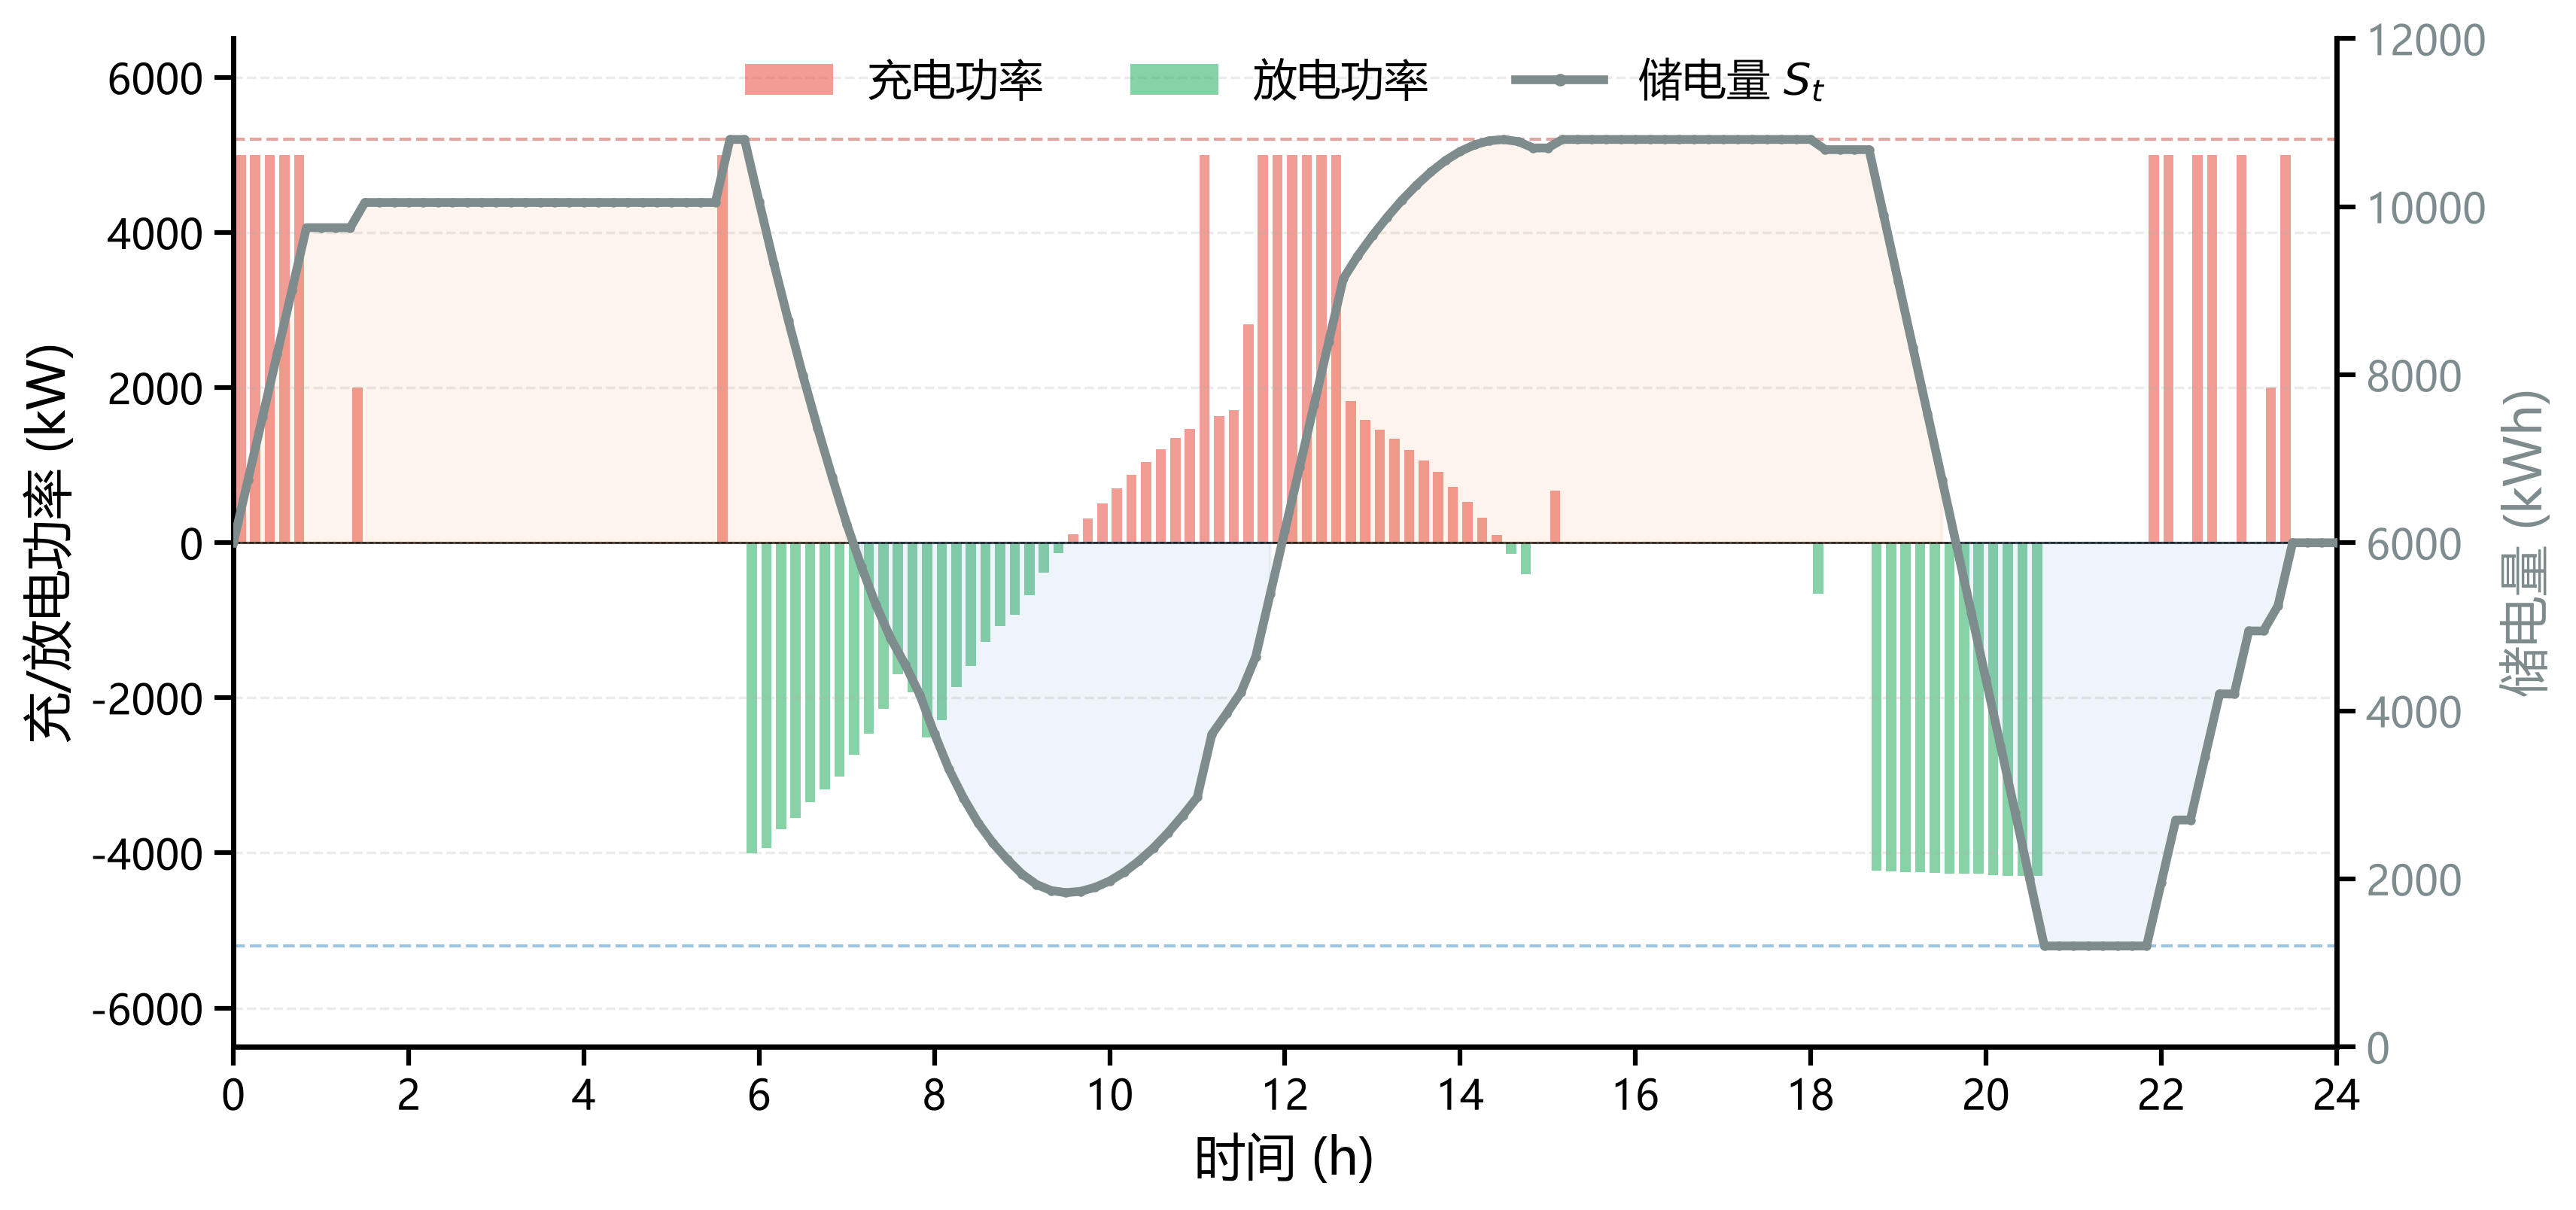
\includegraphics[width=.7\textwidth]{figures/第一问储能充放电.png}
		\caption{问题一储能设备充放电功率与储电量轨迹}
		\label{fig:充放电}
	\end{figure}
	
	如图~\ref{fig:充放电}~所示...
\end{lstlisting}

实际效果：如图~\ref{fig:充放电}~所示（\textcolor{DarkRed}{点击可跳转}）。

引用子图时，使用子图的标签：

实际效果：如图~\ref{fig:sub_left}~和图~\ref{fig:sub_right}~所示，总图编号为图~\ref{fig:电价总}。

\subsubsection{引用公式}

在 \verb|equation| 或 \verb|align| 环境中添加 \verb|\label|：

\begin{lstlisting}
	\begin{equation}
		e^{i\pi} + 1 = 0
		\label{eq:欧拉公式}
	\end{equation}
	
	由式~\eqref{eq:欧拉公式}~可得...
\end{lstlisting}

实际效果：由式~\eqref{eq:欧拉公式}~可得（\textcolor{DarkRed}{点击可跳转}）。

\textbf{注意：}
\begin{itemize}
	\item \verb|\ref{eq:欧拉公式}| 输出：\ref{eq:欧拉公式}（无括号）
	\item \verb|\eqref{eq:欧拉公式}| 输出：\eqref{eq:欧拉公式}（带括号，推荐用于公式引用）
	\item 在 \verb|align| 环境中，每行都可以单独添加 \verb|\label|，引用对应行的编号。
\end{itemize}

\subsubsection{引用页码}

使用 \verb|\pageref| 输出对象所在页码：

\begin{lstlisting}
	该表格位于第~\pageref{tab:预处理统计}~页。
\end{lstlisting}

实际效果：表~\ref{tab:预处理统计}~位于第~\pageref{tab:预处理统计}~页。

\subsubsection{引用参考文献}

使用 \verb|\cite| 或自定义的 \verb|\upcite|（上标引用）：

\begin{lstlisting}
	LaTeX 是一款强大的排版软件\cite{ref1}，真的很强大\upcite{ref1}！
\end{lstlisting}

实际效果：LaTeX 是一款强大的排版软件\cite{ref1}，真的很强大\upcite{ref1}！（\textcolor{DarkRed}{点击可跳转至文末参考文献}）。


标签命名总结：

\begin{center}
	\setlength{\tabcolsep}{12pt}
	\renewcommand{\arraystretch}{1.5}
	\begin{tabular}{ll}
		\toprule
		\textbf{对象类型} & \textbf{推荐前缀} \\
		\midrule
		章节 & \verb|sec:|（如 \verb|sec:daoyan|） \\
		表格 & \verb|tab:|（如 \verb|tab:score|） \\
		图片 & \verb|fig:|（如 \verb|fig:充放电|） \\
		公式 & \verb|eq:|（如 \verb|eq:欧拉公式|） \\
		定理 & \verb|thm:|（如 \verb|thm:中值定理|） \\
		\bottomrule
	\end{tabular}
\end{center}

另外注意，在“第”与 \verb|\ref| 之间、“图”与 \verb|\ref| 之间，应使用波浪号 \verb|~| 连接：

\begin{lstlisting}
	如图~\ref{fig:充放电}~所示...
\end{lstlisting}

\verb|~| 是不可断行空格，防止“图”和编号被分到两行。若不加 \verb|~|，可能出现“图”在行尾、编号在下一行开头的情况。

\textbf{总结：}

\begin{center}
	\setlength{\tabcolsep}{10pt}
	\renewcommand{\arraystretch}{1.5}
	\begin{tabular}{llll}
		\toprule
		\textbf{命令} & \textbf{输出} & \textbf{适用场景} & \textbf{本教程示例} \\
		\midrule
		\verb|\ref{...}| & 编号 & 章节、图、表 & 第~\ref{sec:daoyan}~章、表~\ref{tab:score} \\
		\verb|\eqref{...}| & 带括号编号 & 公式 & \eqref{eq:欧拉公式} \\
		\verb|\pageref{...}| & 页码 & 指出页码 & 第~\pageref{tab:预处理统计}~页 \\
		\verb|\cite{...}| & 文献编号 & 参考文献 & \cite{ref1} \\
		\bottomrule
	\end{tabular}
\end{center}


除了上述基于 \verb|\label| 和 \verb|\ref| 的内部交叉引用外，\LaTeX{} 还支持使用 \verb|\cite| 引用外部的参考文献。关于参考文献的生成与上标引用，详见下一节。

% ============================================================
\section{参考文献及其引用}
\label{sec:ref}
% ============================================================

\subsection{简单的参考文献环境}
在论文或报告末尾，通常需要列出参考文献。对于不需要复杂数据库管理的简单文档，\LaTeX{} 提供了 \verb|thebibliography| 环境来手动管理参考文献。

请将以下代码放在 \verb|\end{document}| \textbf{之前}（即正文的最末尾）：

\begin{lstlisting}
% 强制列出所有文献（即使正文中未引用）
\nocite{*}
\begin{thebibliography}{9}
	\bibitem{ref1} 刘海洋. LaTeX 入门[M]. 北京: 电子工业出版社, 2013.
	\bibitem{ref2} 石继楷. LaTeX零基础入门教程[EB/OL].
	\bibitem{ref3} 石继楷. LaTeX画图教程[EB/OL].
\end{thebibliography}
\end{lstlisting}

\textbf{参数说明：}
\begin{itemize}
\item \verb|\begin{thebibliography}{9}|：花括号中的 \verb|9| 表示参考文献编号的最大宽度（即预留一位数的宽度，如 [1]~[9]）。若文献超过 $9$ 篇，可改为 \verb|99|。
	\item \verb|\bibitem{标签}|：定义一条参考文献，\verb|标签| 用于在正文中引用。
	\item \verb|\nocite{*}|：强制在文末列出所有 \verb|\bibitem|。若不加此命令，只有正文中被引用过的文献才会显示在文末。
\end{itemize}

\subsection{在正文中引用参考文献}
在正文中引用参考文献，使用 \verb|\cite{标签}| 命令。

\begin{lstlisting}
	LaTeX 是一款强大的排版软件\cite{ref1}。
\end{lstlisting}

编译效果：LaTeX 是一款强大的排版软件\cite{ref1}{\color{DarkRed} $\leftarrow$点这里可以跳转至文末参考文献处}

\textbf{上标引用（中文论文常用）：}
在中文学术论文中，参考文献编号通常以\textbf{上标}形式出现。本教程在导言区自定义了 \verb|\upcite| 命令，可以直接生成上标引用：

\begin{lstlisting}
	% 请在导言区添加以下自定义命令：
	\newcommand{\upcite}[1]{\textsuperscript{\textsuperscript{\cite{#1}}}}
	
	% 正文中使用：
	LaTeX 是一款强大的排版软件\upcite{ref1}。
\end{lstlisting}

编译效果：LaTeX 是一款强大的排版软件\upcite{ref1}{\color{DarkRed} $\nwarrow$点这里可以跳转至文末参考文献处}

\textbf{注意：}若需同时引用多篇文献，可用逗号分隔标签：\verb|\upcite{ref2,ref3}|，编译效果为\upcite{ref2,ref3}{\color{DarkRed} $\nwarrow$点这里可以跳转至文末参考文献处}



% ============================================================
\section{导言区详解}
\label{sec:daoyan}
% ============================================================

现在你已经会用前面的模板写文档了，下面逐行解释导言区中每个宏包和命令的作用，方便你按需增删。

\subsection{文档类与页面设置}

\begin{center}
	\setlength{\tabcolsep}{10pt}
	\renewcommand{\arraystretch}{1.2}
	\begin{tabular}{ll}
		\toprule
		\textbf{代码} & \textbf{作用} \\
		\midrule
		\verb|\documentclass{article}| & 声明文档类型为“文章”（适合论文、报告、笔记） \\
		\verb|\usepackage{geometry}| & 加载页面布局宏包 \\
		\verb|\geometry{a4paper,left=2.5cm,...}| & 设置 A4 纸，四边 $2.5$ cm 边距，页眉高度 $13.6$ pt \\
		\bottomrule
	\end{tabular}
\end{center}

\subsection{中文支持与字体}

\begin{center}
	\setlength{\tabcolsep}{2pt}
	\renewcommand{\arraystretch}{1.2}
	\begin{tabular}{ll}
		\toprule
		\textbf{代码} & \textbf{作用} \\
		\midrule
		\verb|\usepackage[UTF8, scheme=plain]{ctex}| & 中文支持。\verb|UTF8| 指定编码；\verb|plain| 使章节标题不显示“第X章” \\
		\verb|\usepackage{fontspec}| & 字体选择宏包（XeLaTeX / LuaLaTeX 编译时必需） \\
		\verb|\setmainfont{Times New Roman}| & 英文正文字体设为 Times New Roman \\
		\bottomrule
	\end{tabular}
\end{center}

\subsection{数学与符号}

\begin{center}
	\setlength{\tabcolsep}{10pt}
	\renewcommand{\arraystretch}{1.2}
	\begin{tabular}{ll}
		\toprule
		\textbf{代码} & \textbf{作用} \\
		\midrule
		\verb|\usepackage{amsmath}| & 数学核心宏包（\verb|align|、\verb|cases|、\verb|equation| 等环境） \\
		\verb|\usepackage{amssymb}| & 额外数学符号（$\mathbb{R}$、$\varnothing$、$\subsetneq$ 等） \\
		\verb|\usepackage{mathrsfs}| & 手写体字母（如 $\mathscr{A}$、$\mathscr{F}$） \\
		\verb|\usepackage{bm}| & 加粗数学符号（如 $\bm{\alpha}$、$\bm{v}$） \\
		\bottomrule
	\end{tabular}
\end{center}

\subsection{表格与图形}

\begin{center}
	\setlength{\tabcolsep}{10pt}
	\renewcommand{\arraystretch}{1.2}
	\begin{tabular}{ll}
		\toprule
		\textbf{代码} & \textbf{作用} \\
		\midrule
		\verb|\usepackage{booktabs}| & 三线表命令（\verb|\toprule|、\verb|\midrule|、\verb|\bottomrule|） \\
		\verb|\usepackage{array}| & 增强表格列格式（支持 \verb|p{}|、\verb|m{}| 等列类型） \\
		\verb|\usepackage{multirow}| & 合并行（\verb|\multirow| 命令） \\
		\verb|\usepackage{colortbl}| & 表格行/单元格背景色（\verb|\rowcolor| 命令） \\
		\verb|\usepackage{graphicx}| & 插入外部图片（\verb|\includegraphics| 命令） \\
		\verb|\usepackage{subcaption}| & 子图环境（\verb|subfigure| 环境，生成图 1(a)、图 1(b) 等编号） \\
		\bottomrule
	\end{tabular}
\end{center}

\subsection{列表与排版}

\begin{center}
	\setlength{\tabcolsep}{10pt}
	\renewcommand{\arraystretch}{1.2}
	\begin{tabular}{ll}
		\toprule
		\textbf{代码} & \textbf{作用} \\
		\midrule
		\verb|\usepackage{enumitem}| & 自定义列表编号样式（如 \verb|label=\arabic*.|、\verb|left=0pt|） \\
		\verb|\usepackage{setspace}| & 行距控制宏包 \\
		\verb|\onehalfspacing| & 设置全文行距为 $1.5$ 倍 \\
		\verb|\setlength{\parskip}{4pt}| & 段落之间添加 $4$ pt 的垂直间距 \\
		\bottomrule
	\end{tabular}
\end{center}

\subsection{画图}

\begin{center}
	\setlength{\tabcolsep}{10pt}
	\renewcommand{\arraystretch}{1.2}
	\begin{tabular}{ll}
		\toprule
		\textbf{代码} & \textbf{作用} \\
		\midrule
		\verb|\usepackage{tikz}| & TikZ 绘图引擎 \\
		\verb|\usepackage{tikz-3dplot}| & 三维绘图辅助（三维坐标系、多面体等） \\
		\verb|\usetikzlibrary{...}| & 加载 TikZ 扩展库 \\
		\bottomrule
	\end{tabular}
\end{center}

\textbf{已加载的 TikZ 库说明：}

\begin{center}
	\setlength{\tabcolsep}{10pt}
	\renewcommand{\arraystretch}{1.2}
	\begin{tabular}{ll}
		\toprule
		\textbf{库名} & \textbf{用途} \\
		\midrule
		\verb|arrows.meta| & 自定义箭头样式（如 \verb|Stealth|、\verb|Triangle|） \\
		\verb|calc| & 坐标计算（如 \verb|$(A)!0.5!(B)$| 求中点） \\
		\verb|patterns| & 填充图案（斜线、网格等） \\
		\verb|decorations.pathmorphing| & 路径变形装饰（波浪线等） \\
		\verb|backgrounds| & 背景层绘制 \\
		\verb|positioning| & 相对定位（如 \verb|right=1cm of A|） \\
		\verb|fit| & 自动包围盒 \\
		\verb|shapes.geometric| & 几何形状节点（正多边形等） \\
		\verb|intersections| & 求曲线交点 \\
		\verb|through| & 过定点画圆 \\
		\verb|angles| & 角度标注（\verb|\draw pic{angle=...}|） \\
		\verb|quotes| & 在图形上直接标注文字（配合 \verb|angles| 使用） \\
		\verb|plotmarks| & 数据点标记样式 \\
		\bottomrule
	\end{tabular}
\end{center}

\subsection{超链接与目录}

\begin{center}
	\setlength{\tabcolsep}{10pt}
	\renewcommand{\arraystretch}{1.2}
	\begin{tabular}{ll}
		\toprule
		\textbf{代码} & \textbf{作用} \\
		\midrule
		\verb|\usepackage{hyperref}| & 超链接宏包，使目录\verb|\ref|\verb|\cite|\verb|\url| 可点击跳转 \\
		\verb|\hypersetup{...}| & 配置链接颜色（见下表） \\
		\verb|\usepackage{tocloft}| & 自定义目录行间距 \\
		\verb|\setlength{\cftbeforesecskip}{2ex}| & 目录中一级标题前间距 $2$ ex \\
		\verb|\setlength{\cftbeforesubsecskip}{1ex}| & 目录中二级标题前间距 $1$ ex \\
		\verb|\setlength{\cftbeforesubsubsecskip}{1ex}| & 目录中三级标题前间距 $1$ ex \\
		\bottomrule
	\end{tabular}
\end{center}

\textbf{hypersetup 各项说明：}

\begin{center}
	\setlength{\tabcolsep}{10pt}
	\renewcommand{\arraystretch}{1.2}
	\begin{tabular}{ll}
		\toprule
		\textbf{选项} & \textbf{说明} \\
		\midrule
		\verb|colorlinks=true| & 链接以颜色显示（而非方框） \\
		\verb|linkcolor=black| & 内部交叉引用（\verb|\ref|）和目录条目为黑色 \\
		\verb|citecolor=black| & 参考文献引用（\verb|\cite|、\verb|\upcite|）为黑色 \\
		\verb|urlcolor=black| & 网址（\verb|\url|）为黑色 \\
		\verb|filecolor=magenta| & 外部文件链接为品红色 \\
		\bottomrule
	\end{tabular}
\end{center}

\textbf{说明：}将 \verb|citecolor| 和 \verb|urlcolor| 设为黑色，可避免参考文献编号显示为默认绿色、网址显示为默认青色，使打印效果更整洁。

\subsection{代码展示}

\begin{center}
	\setlength{\tabcolsep}{10pt}
	\renewcommand{\arraystretch}{1.2}
	\begin{tabular}{ll}
		\toprule
		\textbf{代码} & \textbf{作用} \\
		\midrule
		\verb|\usepackage{listings}| & 代码高亮环境（\verb|lstlisting|） \\
		\verb|\usepackage{xcolor}| & 颜色定义与使用宏包 \\
		\bottomrule
	\end{tabular}
\end{center}

\textbf{lstset 关键选项说明：}

\begin{center}
	\setlength{\tabcolsep}{10pt}
	\renewcommand{\arraystretch}{1.2}
	\begin{tabular}{ll}
		\toprule
		\textbf{选项} & \textbf{说明} \\
		\midrule
		\verb|language=TeX| & 语法高亮针对 \LaTeX{} 语言 \\
		\verb|numbers=left| & 行号显示在左侧 \\
		\verb|frame=shadowbox| & 代码块外框为阴影框 \\
		\verb|breaklines=true| & 超长行自动换行 \\
		\verb|basicstyle=\ttfamily\normalsize| & 代码字体为等宽、正文字号 \\
		\verb|keywordstyle=\color{NavyBlue}| & 关键字（如 \verb|\begin|）为深蓝色 \\
		\verb|commentstyle=\color{codegreen}| & 注释为绿色 \\
		\verb|escapeinside={/@}{@/}| & 在代码中用 \verb|/@| 和 \verb|@/| 包裹的内容会被当作 \LaTeX{} 公式渲染 \\
		\bottomrule
	\end{tabular}
\end{center}

\subsection{自定义颜色}

导言区定义了六种自定义颜色，用途如下：

\begin{center}
	\setlength{\tabcolsep}{10pt}
	\renewcommand{\arraystretch}{1.2}
	\begin{tabular}{lll}
		\toprule
		\textbf{颜色名} & \textbf{定义} & \textbf{典型用途} \\
		\midrule
		\verb|LightGreen| & \verb|\definecolor{LightGreen}{rgb}{0.9,0.95,0.9}| & 代码区域背景 \\
		\verb|LightBlue| & \verb|\definecolor{LightBlue}{RGB}{229,238,255}| & 表格隔行背景 \\
		\verb|LightPink| & \verb|\definecolor{LightPink}{RGB}{255,229,237}| & 重点标注背景 \\
		\verb|DarkRed| & \verb|\definecolor{DarkRed}{RGB}{169,0,0}| & 强调文字、定理标题 \\
		\verb|DarkGreen| & \verb|\definecolor{DarkGreen}{RGB}{0,110,12}| & 题目、例题标注 \\
		\verb|SkyBlue| & \verb|\definecolor{SkyBlue}{RGB}{0,114,255}| & 分类标签、辅助线 \\
		\bottomrule
	\end{tabular}
\end{center}

\subsection{标题中文化}

\begin{center}
	\setlength{\tabcolsep}{10pt}
	\renewcommand{\arraystretch}{1.2}
	\begin{tabular}{ll}
		\toprule
		\textbf{代码} & \textbf{作用} \\
		\midrule
		\verb|\renewcommand{\figurename}{图}| & 图片标题前缀改为“图”（否则显示“Figure”） \\
		\verb|\renewcommand{\tablename}{表}| & 表格标题前缀改为“表”（否则显示“Table”） \\
		\verb|\renewcommand{\refname}{参考文献}| & 参考文献标题改为“参考文献”（否则显示“References”） \\
		\bottomrule
	\end{tabular}
\end{center}

\textbf{说明：}在某些编译环境下，\verb|ctex| 宏包可能未自动将这三个命令设为中文。手动重定义可确保标题始终显示中文。

\subsection{图表标题格式}

\begin{center}
	\setlength{\tabcolsep}{10pt}
	\renewcommand{\arraystretch}{1.2}
	\begin{tabular}{ll}
		\toprule
		\textbf{代码} & \textbf{作用} \\
		\midrule
		\verb|\usepackage{caption}| & 标题格式自定义宏包 \\
		\verb|\captionsetup[table]{...}| & 表格标题：居中、标签后加空格、加粗 \\
		\verb|\captionsetup[figure]{...}| & 图片标题：同上 \\
		\verb|\captionsetup[subfigure]{...}| & 子图标题：加粗 \\
		\bottomrule
	\end{tabular}
\end{center}

\textbf{captionsetup 选项说明：}

\begin{itemize}
	\item \verb|justification=centering|：标题文字居中。
	\item \verb|labelsep=quad|：编号与标题之间用一个 \verb|\quad| 间距分隔（如“图 1\quad 标题”）。
	\item \verb|font={bf}|：标题文字加粗。
\end{itemize}

\subsection{自定义命令}

\begin{center}
	\setlength{\tabcolsep}{10pt}
	\renewcommand{\arraystretch}{1.2}
	\begin{tabular}{ll}
		\toprule
		\textbf{代码} & \textbf{作用} \\
		\midrule
		\verb|\newcommand{\upcite}[1]{...}| & 定义上标引用命令，使参考文献编号以上标形式显示（如$^{\text{[1]}}$）\\
		\verb|\urlstyle{rm}| & 使 \verb|\url| 输出的网址使用罗马正体（默认为等宽字体） \\
		\bottomrule
	\end{tabular}
\end{center}

\subsection{宏包加载顺序说明}

导言区中宏包的加载顺序有一定讲究：

\begin{enumerate}[label=\arabic*., left=0pt]
	
	\item \verb|geometry| 最先加载，确定页面尺寸。
	\item \verb|ctex| 和 \verb|fontspec| 紧随其后，建立中文和字体环境。
	\item 数学、表格、图形等功能宏包居中。
	\item \verb|hyperref| 应尽量靠后加载（它需要知道前面所有宏包的信息来生成正确的超链接）。
	\item 颜色定义、\verb|lstset|、\verb|captionsetup| 等配置放在最后，因为它们可能依赖前面加载的宏包。
	
\end{enumerate}

\textbf{注意：}\verb|hyperref| 之后若再加载其他修改引用行为的宏包，可能导致链接失效。因此，除 \verb|tocloft| 等少数宏包外，\verb|hyperref| 通常是倒数第二个加载的宏包。

\subsection{编译环境与字体问题}

\LaTeX{} 文档能否正常编译，取决于你使用的\textbf{编辑器}和\textbf{编译器}。不同环境下，中文字体的处理方式有显著差异。

\textbf{三种编译器对比：}

\begin{center}
	\setlength{\tabcolsep}{10pt}
	\renewcommand{\arraystretch}{1.5}
	\begin{tabular}{lc}
		\toprule
		\textbf{编译器} & \textbf{特点} \\
		\midrule
		PDFLaTeX & 速度快，但不支持 \verb|\setmainfont|，中文需依赖 \verb|ctex| 内置字体集 \\
		XeLaTeX & 支持系统字体调用，\textbf{推荐用于中文文档} \\
		LuaLaTeX & 功能最强大，兼容 XeLaTeX 的字体特性，速度稍慢 \\
		\bottomrule
	\end{tabular}
\end{center}

本教程的导言区使用了 \verb|\setmainfont{Times New Roman}|，因此\textbf{必须用 XeLaTeX 或 LuaLaTeX 编译}，PDFLaTeX 会直接报错。

\subsubsection{本地编译（Windows / macOS）}

本地编译时，\LaTeX{} 可以直接调用操作系统中安装的字体。

\begin{itemize}
	\item Windows 自带：宋体（SimSun）、黑体（SimHei）、楷体（KaiTi）、仿宋（FangSong）。
	\item macOS 自带：苹方（PingFang SC）、华文宋体（STSong）、华文黑体（STHeiti）。
\end{itemize}

导言区中 \verb|\usepackage[UTF8, scheme=plain]{ctex}| 会自动检测操作系统并选择对应字体集，通常无需额外配置。

\subsubsection{Overleaf 在线编译}

Overleaf 的服务器运行在 Linux 系统上，\textbf{没有预装}宋体、黑体、楷体等 Windows 中文字体。这会导致以下问题：

\begin{itemize}
	\item \verb|\setmainfont{Times New Roman}| 可能报错（Overleaf 有 Times New Roman 的替代品，但名称可能不同）。
	\item 若手动指定 \verb|\setCJKmainfont{SimSun}| 等命令，会提示“字体未找到”。
\end{itemize}

\textbf{解决方案：}

\begin{enumerate}[label=\arabic*., left=0pt]
	
	\item 不要手动指定中文字体，让 \verb|ctex| 自动选择：
	
	\begin{lstlisting}
		% 在 Overleaf 上，只需写这一行，不要加 \setCJKmainfont
		\usepackage[UTF8, scheme=plain]{ctex}
	\end{lstlisting}
	
	\item 若需要指定字体集，使用 \verb|fontset| 选项：
	
	\begin{lstlisting}
		% Overleaf 推荐：使用 fandol 字体集（开源，无需安装）
		\usepackage[UTF8, scheme=plain, fontset=fandol]{ctex}
	\end{lstlisting}
	
	\item 将编译器切换为 XeLaTeX：点击左上角“Menu” $\to$ “Compiler” $\to$ 选择“XeLaTeX”。
	
\end{enumerate}

\textbf{fontset 选项一览：}

\begin{center}
	\setlength{\tabcolsep}{10pt}
	\renewcommand{\arraystretch}{1.6}
	\begin{tabular}{ll}
		\toprule
		\textbf{选项} & \textbf{说明} \\
		\midrule
		\verb|fontset=windows| & 调用 Windows 系统字体（仅限本地编译） \\
		\verb|fontset=macnew| & 调用 macOS 系统字体（仅限本地编译） \\
		\verb|fontset=fandol| & 使用开源 Fandol 字体，\textbf{Overleaf 推荐} \\
		\verb|fontset=none| & 不加载任何中文字体，需手动指定（高级用法） \\
		\bottomrule
	\end{tabular}
\end{center}

\subsubsection{常见报错与排查}

\begin{itemize}
	\item \textbf{报错：}\verb|Font "SimSun" cannot be found.|
	\textbf{原因：}当前系统（或服务器）没有安装该字体。
	\textbf{解决：}改用 \verb|fontset=fandol|，或删除手动指定字体的命令。
	
	\item \textbf{报错：}\verb|\setmainfont undefined.|
	\textbf{原因：}使用了 PDFLaTeX 编译。
	\textbf{解决：}切换为 XeLaTeX。
	
	\item \textbf{报错：}\verb|Emergency stop.| 且提示字体相关。
	\textbf{原因：}通常是字体名称拼写错误，或该字体未安装。
	\textbf{解决：}检查字体名称拼写，或改用系统默认字体。
	
	\item \textbf{中文显示为方框或乱码。}
	\textbf{原因：}未加载 \verb|ctex| 宏包，或文件编码不是 UTF-8。
	\textbf{解决：}确保导言区有 \verb|\usepackage[UTF8]{ctex}|，且文件以 UTF-8 编码保存。
\end{itemize}

\subsubsection{本教程导言区在不同环境的适配}

\begin{center}
	\setlength{\tabcolsep}{10pt}
	\renewcommand{\arraystretch}{1.6}
	\begin{tabular}{lp{11.7cm}}
		\toprule
		\textbf{环境} & \textbf{建议修改} \\
		\midrule
		本地 Windows + XeLaTeX & 导言区原样使用，无需修改 \\
		本地 macOS + XeLaTeX & 导言区原样使用，无需修改 \\
		Overleaf + XeLaTeX & 将 \verb|ctex| 改为 \verb|[UTF8, scheme=plain, fontset=fandol]|；\newline 将 \verb|\setmainfont{Times New Roman}| 改为 \verb|\setmainfont{TeX Gyre Termes}| \\
		\bottomrule
	\end{tabular}
\end{center}

\textbf{注意：}\verb|TeX Gyre Termes| 是 Times New Roman 的开源替代品，Overleaf 预装了该字体，视觉效果与 Times New Roman 几乎一致。

% ============================================================
\section{TikZ 画图入门}
% ============================================================

\subsection{引言}

本章使用 \texttt{TikZ} 与 \texttt{tikz-3dplot} 宏包，从零开始讲解如何在 \LaTeX{} 中绘制数学图形。内容包括：
\begin{itemize}
	\item 平面图形：直线、坐标系、三角形、圆、椭圆、抛物线、双曲线以及各种标注技巧。
	\item 三维图形：三维坐标系、空间点、直线、平面、多面体、旋转体（线框示意）等。
\end{itemize}

\subsection{平面绘图基础}

使用 \verb|\draw| 绘制直线。标记点有两种方式：
\begin{itemize}
	\item \textbf{直接标记}：\verb|\fill (0,0) circle (2pt);| 画一个点，但该点没有名称，后续无法引用。
	\item \textbf{命名后批量标记}：先用 \verb|\coordinate| 定义点，再用 \verb|\foreach| 统一画点。
\end{itemize}

\textbf{推荐做法}：对于会被多次引用的点，务必命名；对于只用一次的点，可直接用 \verb|\fill|。

\begin{lstlisting}
	\begin{tikzpicture}
		% 命名点
		\coordinate (A) at (0,0);
		\coordinate (B) at (4,0);
		\coordinate (C) at (1,3);
		% 画三角形
		\draw (A) -- (B) -- (C) -- cycle;
		% 批量标记所有点
		\foreach \p/\pos in {A/below left,B/below right,C/above}
		\fill (\p) circle (2pt) node[\pos] {$\p$};
	\end{tikzpicture}
\end{lstlisting}

\begin{center}
	\begin{tikzpicture}
		
		\coordinate (A) at (0,0);
		\coordinate (B) at (4,0);
		\coordinate (C) at (1,3);
		\draw (A) -- (B) -- (C) -- cycle;
		\foreach \p/\pos in {A/below left,B/below right,C/above}
		\fill (\p) circle (2pt) node[\pos] {$\p$};
		
	\end{tikzpicture}
\end{center}

\subsection{坐标系与网格}

\begin{lstlisting}
	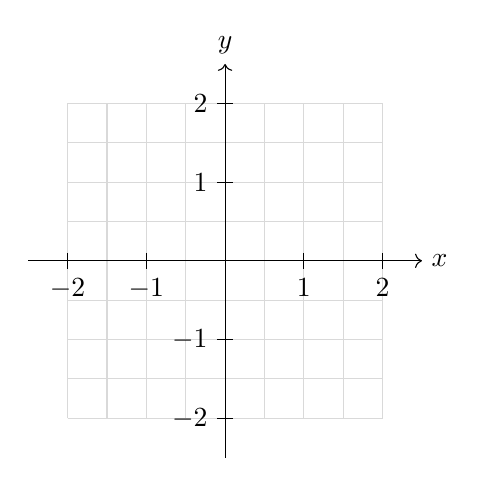
\begin{tikzpicture}
		\draw[step=0.5, gray!30, thin] (-2,-2) grid (2,2);
		\draw[->] (-2.5,0) -- (2.5,0) node[right] {$x$};
		\draw[->] (0,-2.5) -- (0,2.5) node[above] {$y$};
		\foreach \x in {-2,-1,1,2}
		\draw (\x,0.1) -- (\x,-0.1) node[below] {$\x$};
		\foreach \y in {-2,-1,1,2}
		\draw (0.1,\y) -- (-0.1,\y) node[left] {$\y$};
	\end{tikzpicture}
\end{lstlisting}

\begin{center}
	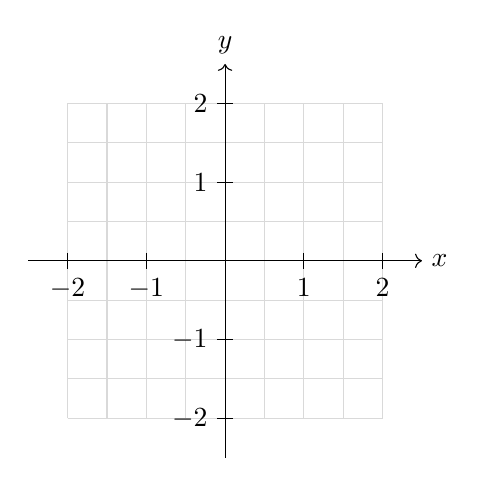
\begin{tikzpicture}
		
		\draw[step=0.5, gray!30, thin] (-2,-2) grid (2,2);
		\draw[->] (-2.5,0) -- (2.5,0) node[right] {$x$};
		\draw[->] (0,-2.5) -- (0,2.5) node[above] {$y$};
		\foreach \x in {-2,-1,1,2}
		\draw (\x,0.1) -- (\x,-0.1) node[below] {$\x$};
		\foreach \y in {-2,-1,1,2}
		\draw (0.1,\y) -- (-0.1,\y) node[left] {$\y$};
		
	\end{tikzpicture}
\end{center}

\subsection{三角形与辅助线}

\begin{lstlisting}
	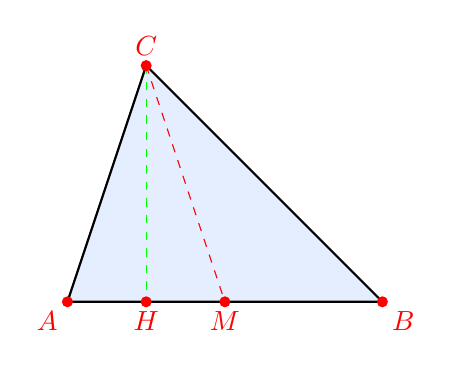
\begin{tikzpicture}
		\coordinate (A) at (0,0);
		\coordinate (B) at (4,0);
		\coordinate (C) at (1,3);
		\fill[LightBlue] (A) -- (B) -- (C) -- cycle;
		\draw[thick] (A) -- (B) -- (C) -- cycle;
		\coordinate (M) at ($(A)!0.5!(B)$);
		\draw[dashed, red] (C) -- (M);
		\coordinate (H) at ($(A)!(C)!(B)$);
		\draw[dashed, green] (C) -- (H);
		\foreach \p/\pos in {A/below left,B/below right,C/above,M/below,H/below}
		\fill[red] (\p) circle (2pt) node[\pos] {$\p$};
	\end{tikzpicture}
\end{lstlisting}

\begin{center}
	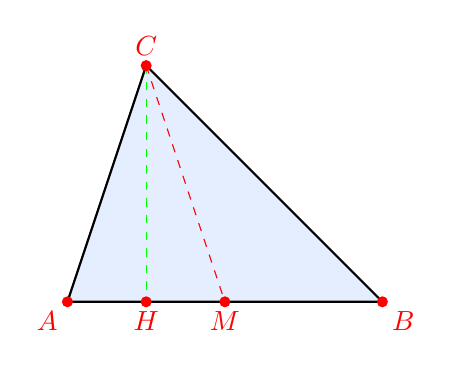
\begin{tikzpicture}
		
		\coordinate (A) at (0,0);
		\coordinate (B) at (4,0);
		\coordinate (C) at (1,3);
		\fill[LightBlue] (A) -- (B) -- (C) -- cycle;
		\draw[thick] (A) -- (B) -- (C) -- cycle;
		\coordinate (M) at ($(A)!0.5!(B)$);
		\draw[dashed, red] (C) -- (M);
		\coordinate (H) at ($(A)!(C)!(B)$);
		\draw[dashed, green] (C) -- (H);
		\foreach \p/\pos in {A/below left,B/below right,C/above,M/below,H/below}
		\fill[red] (\p) circle (2pt) node[\pos] {$\p$};
		
	\end{tikzpicture}
\end{center}

\subsection{角度标注}

使用 \texttt{angles} 和 \texttt{quotes} 库标注角度：

\begin{lstlisting}
	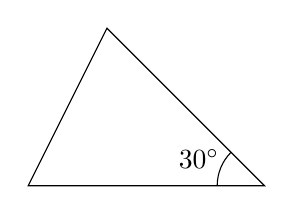
\begin{tikzpicture}
		\coordinate (A) at (0,0);
		\coordinate (B) at (3,0);
		\coordinate (C) at (1,2);
		\draw (A) -- (B) -- (C) -- cycle;
		\draw pic["$30^\circ$", draw, angle eccentricity=1.5, angle radius=0.6cm]
		{angle = C--B--A};
	\end{tikzpicture}
\end{lstlisting}

\begin{center}
	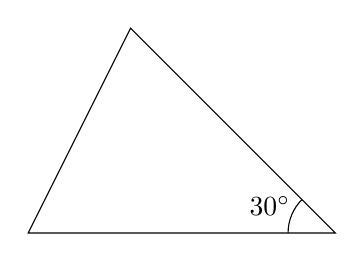
\begin{tikzpicture}[scale=1.3]
		
		\coordinate (A) at (0,0);
		\coordinate (B) at (3,0);
		\coordinate (C) at (1,2);
		\draw (A) -- (B) -- (C) -- cycle;
		\draw pic["$30^\circ$", draw, angle eccentricity=1.5, angle radius=0.6cm]
		{angle = C--B--A};
		
	\end{tikzpicture}
\end{center}

\subsection{圆锥曲线}

\subsubsection{圆}

\begin{lstlisting}
	\draw[thick, red] (0,0) circle (2);
\end{lstlisting}

\begin{center}
	\begin{tikzpicture}[scale=0.8]
		
		\draw[->] (-3,0) -- (3,0) node[right] {$x$};
		\draw[->] (0,-3) -- (0,3) node[above] {$y$};
		\draw[thick, red] (0,0) circle (2);
		\fill (0,0) circle (1pt) node[below left] {$O$};
		
	\end{tikzpicture}
\end{center}

\subsubsection{椭圆}

\begin{lstlisting}
	\draw[thick, blue] (0,0) ellipse (2 and 1.2);
\end{lstlisting}

\begin{center}
	\begin{tikzpicture}
		
		\draw[->] (-3,0) -- (3,0) node[right] {$x$};
		\draw[->] (0,-2) -- (0,2) node[above] {$y$};
		\draw[thick, blue] (0,0) ellipse (2 and 1.2);
		
	\end{tikzpicture}
\end{center}

\subsubsection{抛物线}

用参数方程绘制 $y^2=4x$（令 $x=t^2,\ y=2t$）：

\begin{lstlisting}
	\begin{tikzpicture}
		\draw[->] (-1,0) -- (4,0) node[right] {$x$};
		\draw[->] (0,-3) -- (0,3) node[above] {$y$};
		\draw[thick, orange, domain=-1.5:1.5, smooth, variable=\t]
		plot ({\t*\t}, {2*\t});
		\fill (1,0) circle (2pt) node[above] {焦点$(1,0)$};
		\draw[dashed] (-1,-3) -- (-1,3) node[left] {$x=-1$};
	\end{tikzpicture}
\end{lstlisting}

\begin{center}
	\begin{tikzpicture}
		
		\draw[->] (-1,0) -- (4,0) node[right] {$x$};
		\draw[->] (0,-3) -- (0,3) node[above] {$y$};
		\draw[thick, orange, domain=-1.5:1.5, smooth, variable=\t]
		plot ({\t*\t}, {2*\t});
		\fill (1,0) circle (2pt) node[above] {焦点$(1,0)$};
		\draw[dashed] (-1,-3) -- (-1,3) node[left] {$x=-1$};
		
	\end{tikzpicture}
\end{center}

\subsubsection{双曲线}

用 $y$ 作自变量绘制两个分支（避免断点）：

\begin{lstlisting}
	\begin{tikzpicture}
		\draw[->, gray!40] (-4,0) -- (4,0) node[right] {$x$};
		\draw[->, gray!40] (0,-4) -- (0,4) node[above] {$y$};
		% 右支
		\draw[thick, domain=-3.5:3.5, smooth, samples=200, variable=\y]
		plot ({sqrt(\y*\y+1)}, {\y});
		% 左支
		\draw[thick, domain=-3.5:3.5, smooth, samples=200, variable=\y]
		plot ({-sqrt(\y*\y+1)}, {\y});
		% 渐近线
		\draw[dashed, gray!40] (-3.5,-3.5) -- (3.5,3.5);
		\draw[dashed, gray!40] (-3.5,3.5) -- (3.5,-3.5);
	\end{tikzpicture}
\end{lstlisting}

\begin{center}
	\begin{tikzpicture}[scale=0.9]
		
		\draw[->, gray!40] (-4,0) -- (4,0) node[right] {$x$};
		\draw[->, gray!40] (0,-4) -- (0,4) node[above] {$y$};
		\draw[thick, teal, domain=-3.5:3.5, smooth, samples=200, variable=\y]
		plot ({sqrt(\y*\y+1)}, {\y});
		\draw[thick, teal, domain=-3.5:3.5, smooth, samples=200, variable=\y]
		plot ({-sqrt(\y*\y+1)}, {\y});
		\draw[dashed, gray!40] (-3.5,-3.5) -- (3.5,3.5);
		\draw[dashed, gray!40] (-3.5,3.5) -- (3.5,-3.5);
		
	\end{tikzpicture}
\end{center}

\subsection{三维绘图}

\subsubsection{三维坐标系}

\begin{lstlisting}
	\tdplotsetmaincoords{70}{120}
	\begin{tikzpicture}[tdplot_main_coords, scale=2]
		\draw[->] (0,0,0) -- (2,0,0) node[below left]{$x$};
		\draw[->] (0,0,0) -- (0,2,0) node[right]{$y$};
		\draw[->] (0,0,0) -- (0,0,2) node[above]{$z$};
	\end{tikzpicture}
\end{lstlisting}

\tdplotsetmaincoords{70}{120}
\begin{center}
	\begin{tikzpicture}[tdplot_main_coords, scale=1.8]
		
		\draw[->] (0,0,0) -- (2,0,0) node[below left]{$x$};
		\draw[->] (0,0,0) -- (0,2,0) node[right]{$y$};
		\draw[->] (0,0,0) -- (0,0,2) node[above]{$z$};
		
	\end{tikzpicture}
\end{center}

\subsubsection{正方体}

\begin{lstlisting}
	\tdplotsetmaincoords{70}{120}
	\begin{tikzpicture}[tdplot_main_coords, scale=3]
		\coordinate (A) at (0,0,0);
		\coordinate (B) at (1,0,0);
		\coordinate (C) at (1,1,0);
		\coordinate (D) at (0,1,0);
		\coordinate (E) at (0,0,1);
		\coordinate (F) at (1,0,1);
		\coordinate (G) at (1,1,1);
		\coordinate (H) at (0,1,1);
		\draw[thick] (A)--(B)--(C)--(D)--cycle;
		\draw[thick] (E)--(F)--(G)--(H)--cycle;
		\draw[thick] (A)--(E) (B)--(F) (C)--(G) (D)--(H);
		\foreach \p/\pos in {A/above left,B/below left,C/below,D/right,
			E/above,F/left,G/above,H/above right}
		\fill (\p) circle (0.5pt) node[\pos] {$\p$};
	\end{tikzpicture}
\end{lstlisting}

\tdplotsetmaincoords{70}{120}
\begin{center}
	\begin{tikzpicture}[tdplot_main_coords, scale=3]
		
		\coordinate (A) at (0,0,0);
		\coordinate (B) at (1,0,0);
		\coordinate (C) at (1,1,0);
		\coordinate (D) at (0,1,0);
		\coordinate (E) at (0,0,1);
		\coordinate (F) at (1,0,1);
		\coordinate (G) at (1,1,1);
		\coordinate (H) at (0,1,1);
		\draw[thick] (A)--(B)--(C)--(D)--cycle;
		\draw[thick] (E)--(F)--(G)--(H)--cycle;
		\draw[thick] (A)--(E) (B)--(F) (C)--(G) (D)--(H);
		\foreach \p/\pos in {A/above left,B/below left,C/below,D/right,E/above,F/left,G/above,H/above right}
		\fill (\p) circle (0.5pt) node[\pos] {$\p$};
		
	\end{tikzpicture}
\end{center}

\subsection{图文并排（minipage）}

使用 \texttt{minipage} 可以将文档分为左右两部分，一边放文字，一边放图片：

\begin{lstlisting}
	\noindent
	\begin{minipage}[t]{0.6\textwidth}
		
		左边写文字内容。\\
		第二行。
		
	\end{minipage}
	\hfill
	\begin{minipage}[t]{0.35\textwidth}
		
		\begin{tikzpicture}[baseline=(current bounding box.north), scale=1]
			% 画图代码
		\end{tikzpicture}
		
	\end{minipage}
\end{lstlisting}

\noindent
\begin{minipage}[t]{0.6\textwidth}
	
	这里展示如何在左边写内容，图片展示在右边。\\
	使用 minipage 实现。\\
	我们先画了 $\triangle ABC$，\\
	随后作了 $AB$ 的垂线 $CH$，\\
	找到了 $AB$ 的中点 $M$。\\
	$\therefore CH\perp AB$。
	
\end{minipage}
\hfill
\begin{minipage}[t]{0.35\textwidth}
	
	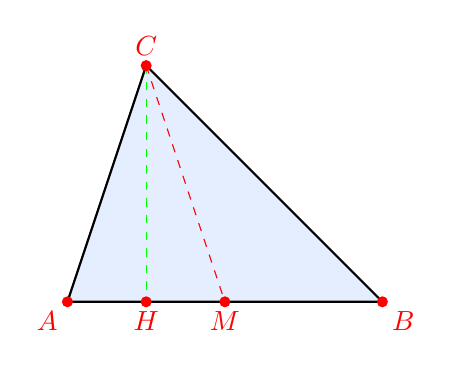
\begin{tikzpicture}[baseline=(current bounding box.north), scale=1]
		
		\coordinate (A) at (0,0);
		\coordinate (B) at (4,0);
		\coordinate (C) at (1,3);
		\fill[LightBlue] (A) -- (B) -- (C) -- cycle;
		\draw[thick] (A) -- (B) -- (C) -- cycle;
		\coordinate (M) at ($(A)!0.5!(B)$);
		\draw[dashed, red] (C) -- (M);
		\coordinate (H) at ($(A)!(C)!(B)$);
		\draw[dashed, green] (C) -- (H);
		\foreach \p/\pos in {A/below left,B/below right,C/above,M/below,H/below}
		\fill[red] (\p) circle (2pt) node[\pos] {$\p$};
		
	\end{tikzpicture}
	
\end{minipage}

\subsection{使用循环绘制多个对象}

利用 \verb|\foreach| 快速绘制多个相似对象：

\begin{lstlisting}
	
\begin{tikzpicture}
		\foreach \x in {1,...,5}
		\fill (\x,0) circle (2pt) node[below] {$\x$};
	\end{tikzpicture}
\end{lstlisting}

\begin{center}
	
\begin{tikzpicture}
		
		\foreach \x in {1,...,5}
		\fill (\x,0) circle (2pt) node[below] {$\x$};
		
	\end{tikzpicture}
\end{center}

% ============================================================
\section{附录：完整模板}

将以下代码保存为 \verb!.tex! 文件，用 XeLaTeX 编译，即可得到本教程使用的完整模板：

\begin{lstlisting}[
escapeinside={|<}{>|},
basicstyle=\ttfamily\footnotesize\linespread{0.9}\selectfont,
aboveskip=0.5ex,
belowskip=0.5ex
]
\documentclass{article}
\usepackage{geometry}
\geometry{
	a4paper,
	left=2.5cm,   
	right=2.5cm,   
	top=2.5cm,      
	bottom=2.5cm,  
	headheight=13.6pt
}

% 最简单、最稳定的中文方案（自动适配系统，永不报错）
\usepackage[UTF8, scheme=plain]{ctex}

% 设置英文默认字体为 Times New Roman
\usepackage{fontspec}
\setmainfont{Times New Roman}

\usepackage{amsmath}
\usepackage{amssymb}
\usepackage{booktabs}
\usepackage{caption}
\usepackage{setspace}
\onehalfspacing
\setlength{\parskip}{4pt}

\usepackage{array}
\usepackage{listings}
\usepackage{graphicx}
\usepackage{enumitem}
\usepackage{subcaption}
\usepackage{multirow}
\usepackage{mathrsfs}
\usepackage{bm}
\usepackage{xcolor}
\usepackage{colortbl}

\usepackage{tikz}
\usepackage{tikz-3dplot}
\usetikzlibrary{
	arrows.meta, 
	calc, 
	patterns, 
	decorations.pathmorphing, 
	backgrounds, 
	positioning, 
	fit, 
	shapes.geometric, 
	intersections, 
	through, 
	angles, 
	quotes,
	plotmarks
}

% 目录与超链接设置
\usepackage{hyperref}
\hypersetup{
	colorlinks=true,
	linkcolor=black,   % 内部交叉引用（如 \ref）和目录颜色
	citecolor=black,   % 参考文献引用（如 \upcite）颜色，解决绿色问题
	urlcolor=black,    % 网址（如 \url）颜色，解决蓝色/青色问题
	filecolor=magenta,
}
\usepackage{tocloft}
\setlength{\cftbeforesecskip}{2ex}
\setlength{\cftbeforesubsecskip}{1ex}
\setlength{\cftbeforesubsubsecskip}{1ex}

% 定义代码颜色
\definecolor{codegreen}{rgb}{0,0.6,0}
\definecolor{NavyBlue}{RGB}{0,0,128}
\definecolor{PineGreen}{RGB}{1,121,111}

% 配置 listings 环境
\lstset{
	language=TeX,
	tabsize=4,
	captionpos=b,
	numbers=left,
	numbersep=1em,
	sensitive=true,
	showtabs=false,
	frame=shadowbox,
	breaklines=true,
	keepspaces=true,
	showspaces=false,
	showstringspaces=false,
	breakatwhitespace=false,
	basicstyle=\ttfamily\normalsize,
	keywordstyle=\color{NavyBlue},
	commentstyle=\color{codegreen},
	numberstyle=\color{black},
	stringstyle=\color{PineGreen!90!black},
	rulesepcolor=\color{red!20!green!20!blue!20},
	escapeinside={/@}{@/},
}

% 自定义颜色
\definecolor{LightGreen}{rgb}{0.9, 0.95, 0.9}
\definecolor{LightBlue}{RGB}{229, 238, 255}
\definecolor{LightPink}{RGB}{255, 229, 237}
\definecolor{DarkRed}{RGB}{169,0,0}
\definecolor{DarkGreen}{RGB}{0,110,12}
\definecolor{SkyBlue}{RGB}{0,114,255}
% 将图表标题和参考文献标题强制设为中文
\renewcommand{\figurename}{图}
\renewcommand{\tablename}{表}
\renewcommand{\refname}{参考文献}
\captionsetup[table]{
	justification=centering,
	labelsep=quad,
	font={bf}
}
\captionsetup[figure]{
	justification=centering,
	labelsep=quad,
	font={bf}
}
\captionsetup[subfigure]{
	font={bf}
}

\newcommand{\upcite}[1]{\textsuperscript{\textsuperscript{\cite{#1}}}}
\urlstyle{rm}

\begin{document}
	你的正文写在这里。
\end{document}
\end{lstlisting}

\nocite{*}
\begin{thebibliography}{9}%宽度9
	\bibitem{ref1} 刘海洋. LaTeX 入门[M]. 北京: 电子工业出版社, 2013.
	\bibitem{ref2} 石继楷. LaTeX零基础入门教程[EB/OL].
	\bibitem{ref3} 石继楷. LaTeX画图教程[EB/OL].
\end{thebibliography}

\end{document}